
\clearpage
\section{Entities}
\label{sec:builder-feature-entities}

An entity in KayanOS is a type of record the organization defines, such as “Maintenance requests” or “Equipment”. The “Entities” page lists every record type grouped by app and section, so you can create a new type or open an existing one to edit it. The “Builder” workspace calls an entity a “record type”; both words mean the same thing.

\textbf{Path and who uses it:} “Builder” → “Core” → “Entities”. Used by the system administrator, or anyone with entity permissions, when the organization needs a record the ready-made apps do not provide.

\begin{rcnote}[Example: Horizon]
Horizon's system administrator searches for a record type for branch visit requests and finds none, so they create a new entity called “Visit requests” and place it in the “Branch services” app. On the image, they start with search ① and then press “Add Entity” ③.
\end{rcnote}

\begin{figure}[H]
\centering
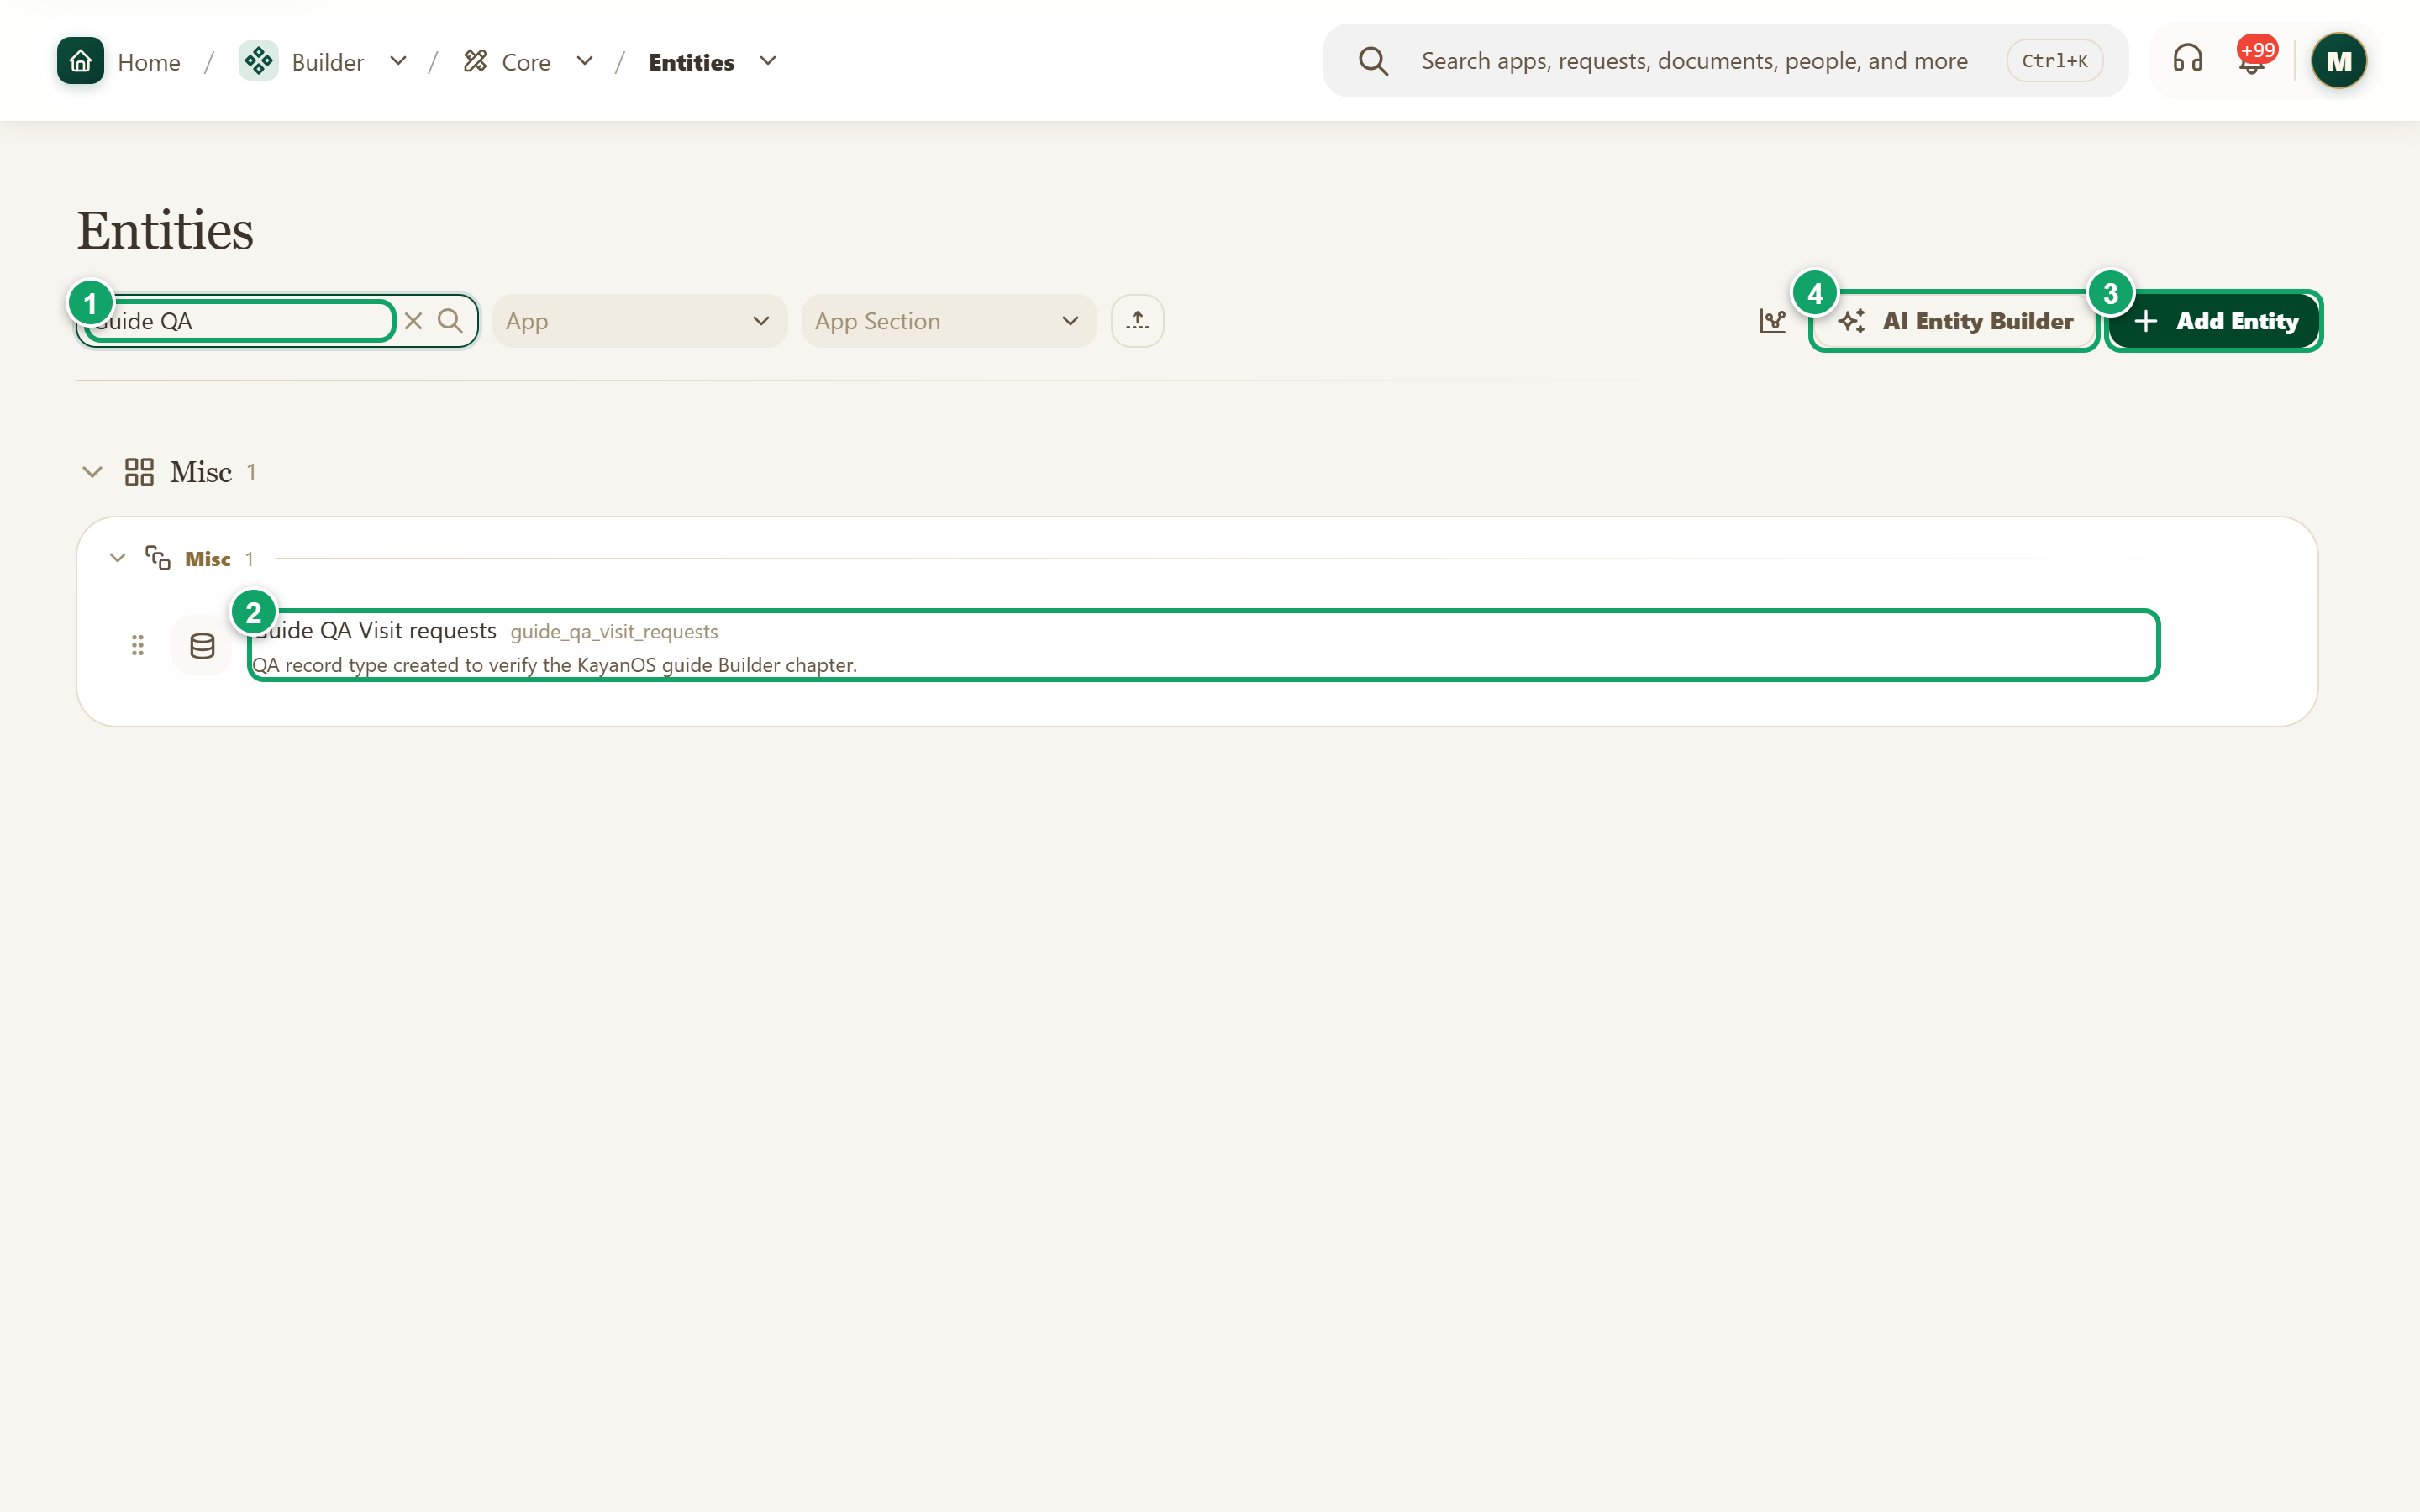
\includegraphics[width=0.95\linewidth,height=0.72\textheight,keepaspectratio]{figures/screens/ch06-entities-en.png}
\caption{The “Entities” page after searching for a record type}
\label{fig:builder-entities-screen}
\shotnote{The page lists record types grouped by app; here search narrowed it to one test record type created on test2 to verify this chapter. ① The search box: type part of the type’s name before creating a new one. ② The type you found: press it to open it in the “Builder” workspace. ③ “Add Entity”: creates a new type when you find nothing suitable. ④ “AI Entity Builder”: proposes fields from a description you write.}
\end{figure}


\begin{table}[H]
\centering
\caption{What do you find here?}
\label{tab:builder-entities-data}
\begin{tabularx}{\linewidth}{R{3.6cm} Y}
\rcHeaderRow
\thh{Section} & \thh{Content and action}\\
List of types & Record types grouped by app and section, each with its name, key and description. Narrow the list with search or the “App” and “App Section” filters.\\
Add Entity & Opens a page where you write the type's title, description and first fields, then press “Create Entity”.\\
AI Entity Builder & Describe the type you need in your own words and the system proposes its fields for you to review before saving. The button appears only when the organization has enabled AI in Builder.\\
View ERD Diagram & Draws the record types and the relationships between them, so you know what a type is linked to before you change it.\\
Open an existing type & Pressing a type opens it in the “Builder” workspace, where you edit its fields, page and lists and publish the changes.\\
\end{tabularx}
\end{table}

\begin{figure}[H]
\centering
\begin{tikzpicture}[node distance=0.5cm]
\node[stepBox] (a) {Look for a similar type};
\node[stepBox,below=of a] (b) {Add Entity, write its title};
\node[stepBox,below=of b] (c) {Create Entity};
\node[stepBox,below=of c] (d) {Open it in Builder};
\draw[flowsTo] (a) -- (b);
\draw[flowsTo] (b) -- (c);
\draw[flowsTo] (c) -- (d);
\end{tikzpicture}
\rclegend
\caption{Creating a record type}
\label{fig:builder-entities-flow}
\shotnote{The diagram starts with a search because the type you need may already exist in a ready-made app, and a second copy splits the data between two places. After “Create Entity” you return to the entity list and open the new type in the “Builder” workspace to finish it; creating the type does not mean the application is ready for the team.}
\end{figure}

\subsection{Steps and check}
\begin{enumerate}
\item Open “Entities”, type a name close to what you need into search, and review the results before creating a new type.
\item Press “Add Entity”, write a plural title that describes the records, such as “Maintenance requests”, and add a short description.
\item Name the suggested first field or change its type, and press “Add New Field” for each other essential piece of information.
\item Press the settings button next to “Create Entity” to choose the app and section where the type appears, then press “Create Entity”.
\end{enumerate}

\textbf{Check and recovery:} a success message should appear and the new type should show in the “Entities” list under the app you chose. If “Create Entity” stays disabled, write the type's title first; if you cannot find the type in the list, clear the app and section filters and search by its name.

\clearpage
\section{Fields}
\label{sec:builder-feature-fields}

A field defines one piece of information each record stores, such as a date, an amount or the person responsible. Choosing the right field type matters: it decides how the value is entered and checked, and allows sorting, filtering and calculation later. You add fields in the “Fields” section of the “Builder” workspace.

\textbf{Path and who uses it:} “Entities” → open the record type → “Fields”. Used by whoever builds the record type, before arranging its page and lists.

\begin{rcnote}[Example: Horizon]
The system administrator adds a “Serial ID” field to “Visit requests” that gives each request a number such as \en{HZN-VR-0001}, then a “Relation” field linking the request to the branch, a “Date” field for the visit date and a “Long Text” field for its purpose. Their steps match numbers ① and ③ on the image.
\end{rcnote}

\begin{figure}[H]
\centering
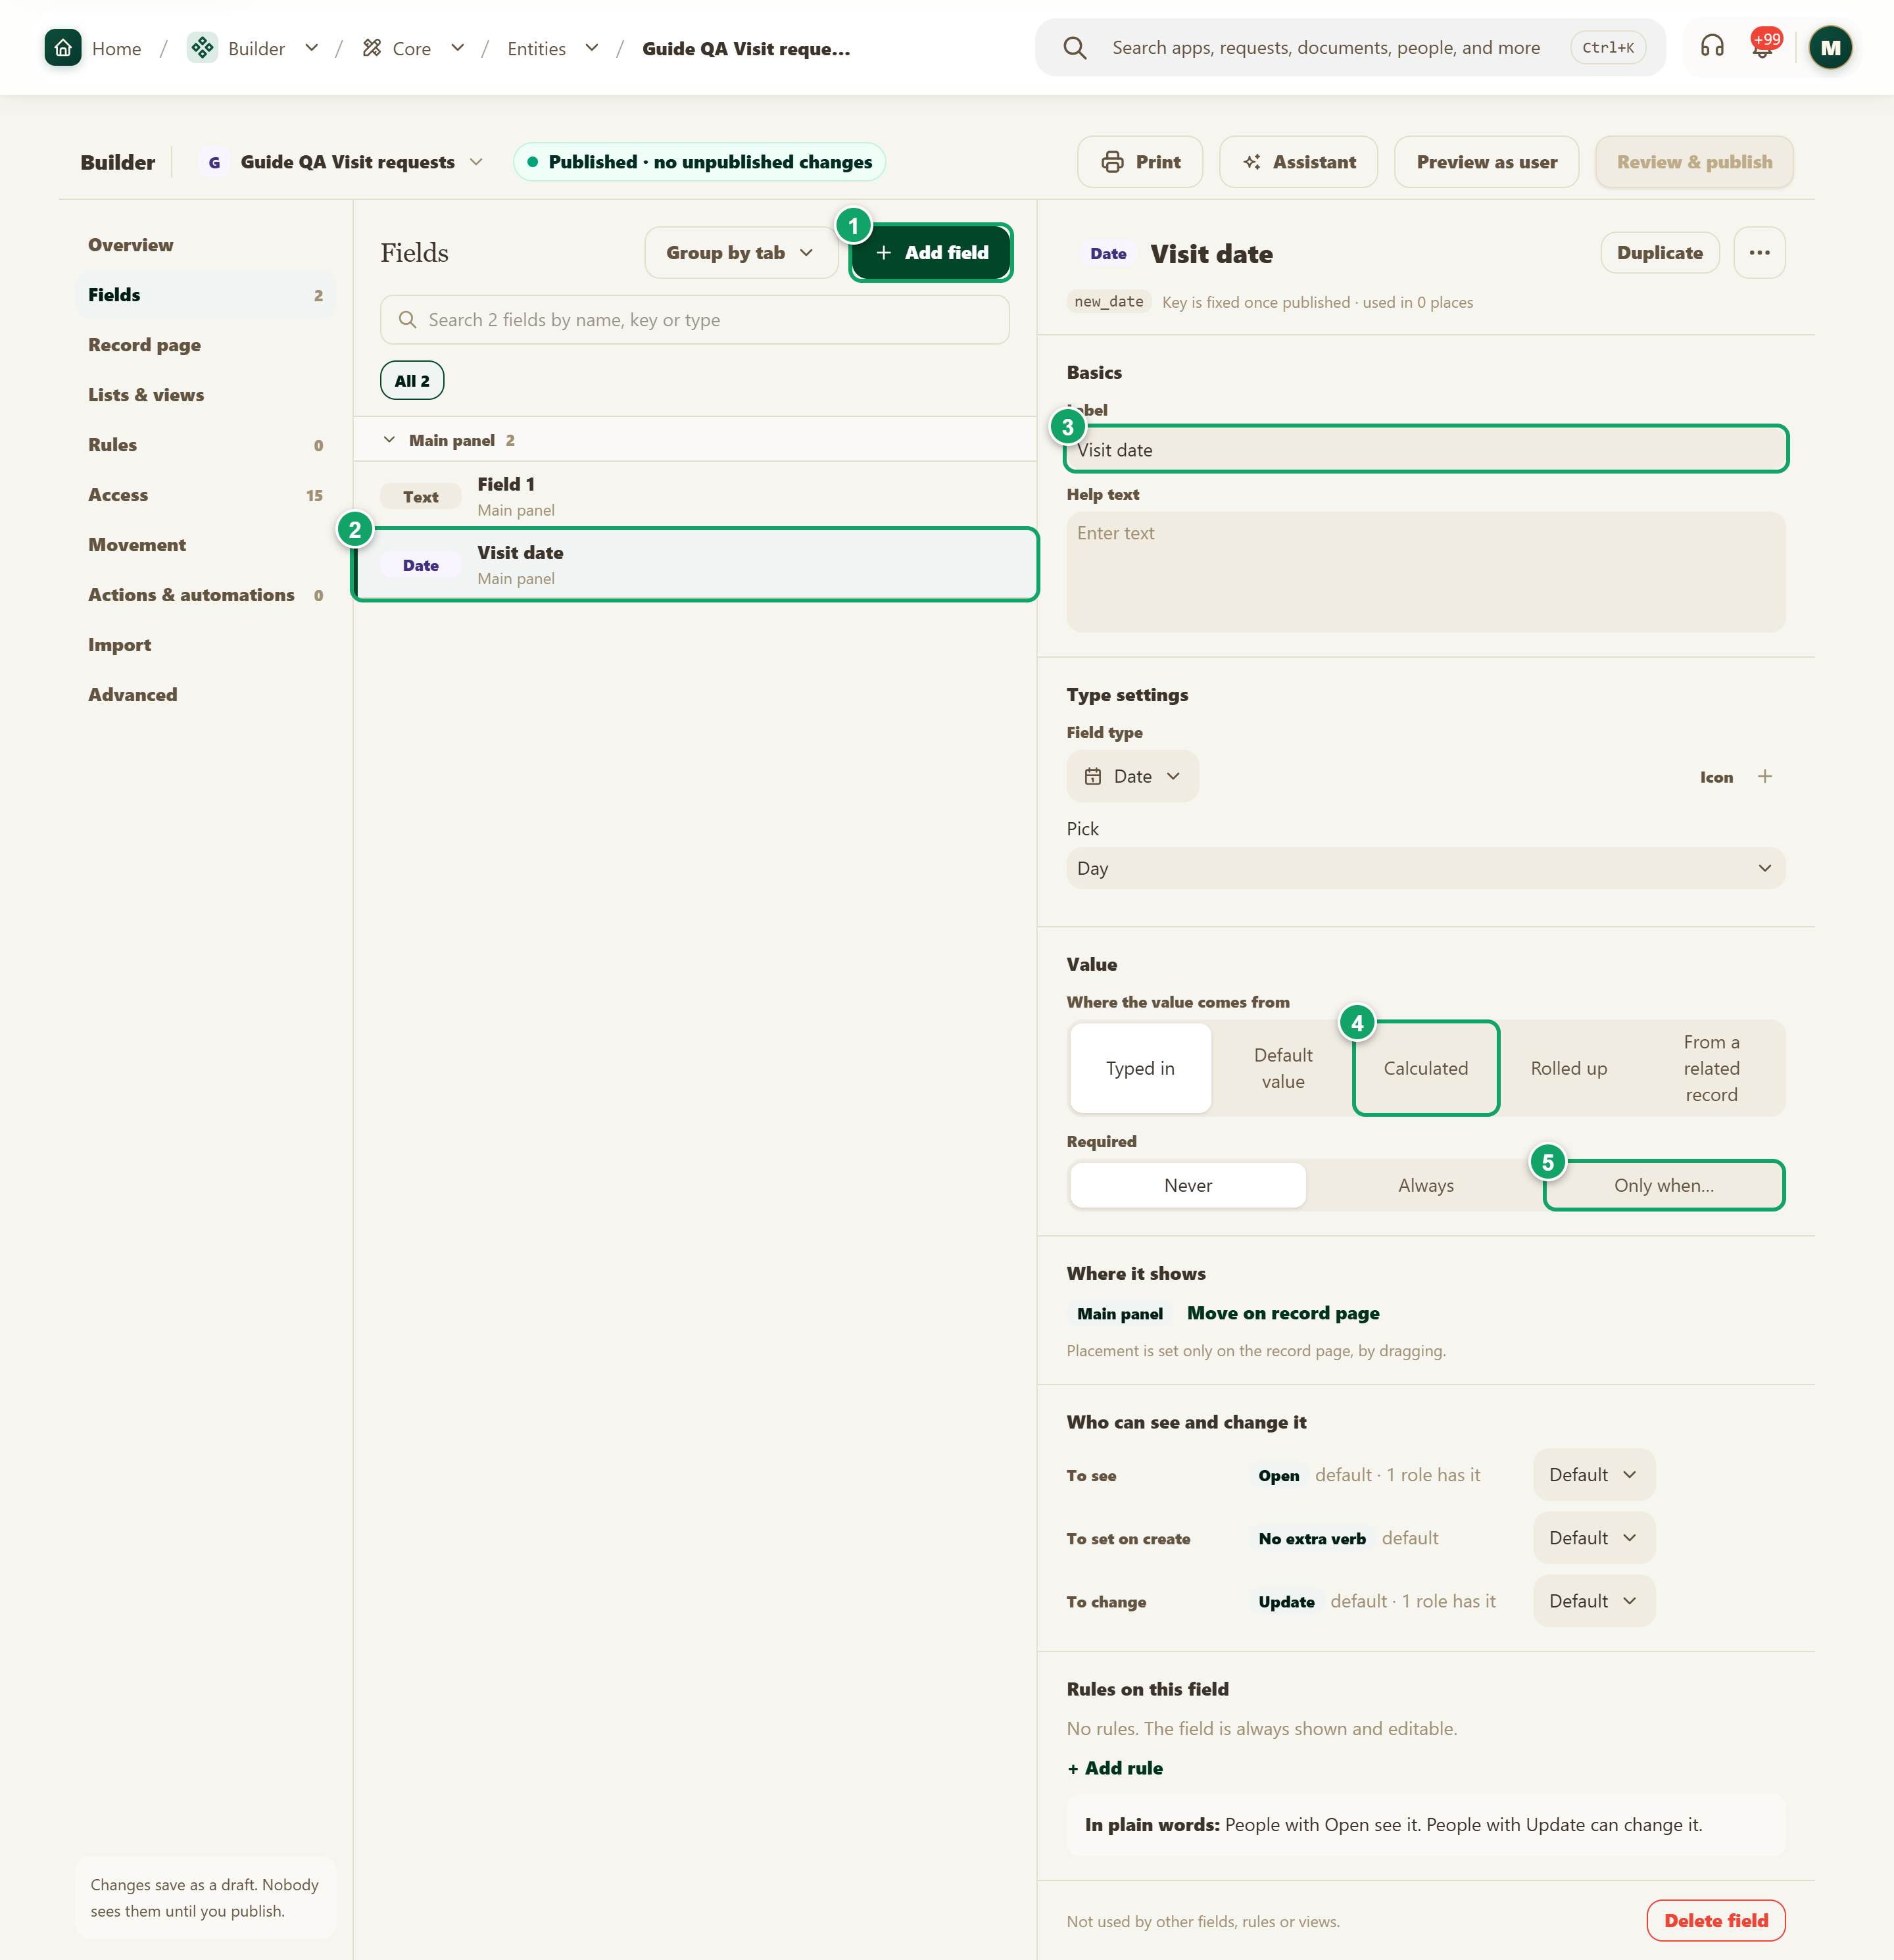
\includegraphics[width=0.95\linewidth,height=0.72\textheight,keepaspectratio]{figures/screens/ch06-ws-fields-en.png}
\caption{The “Fields” section and the settings of a date field}
\label{fig:builder-fields-screen}
\shotnote{The section lists the record type’s fields, and choosing one shows its settings beside it. The selected field is a “Date” field added and published while testing this chapter on test2. ① “Add field”: opens the list of field types. ② The selected field in the list. ③ “Label”: the name users see. ④ “Calculated”: makes the value the result of a formula instead of something users type. ⑤ “Only when…”: makes the field required in a given situation.}
\end{figure}


\begin{table}[H]
\centering
\caption{Field types}
\label{tab:builder-fields-types}
\begin{tabularx}{\linewidth}{R{3.6cm} Y}
\rcHeaderRow
\thh{Group} & \thh{Types and when to use them}\\
Text & “Text” for a short value, “Long Text” for a description, “Rich Text” for formatted text and “Phone” for a phone number.\\
Numbers and IDs & “Number” for quantities and amounts, “Duration” for time spent and “Serial ID” for a reference number the system generates for each record.\\
Dates and times & “Date”, “Date \& Time” and “Time”, plus ranges such as “Date Range” when the information has a start and an end.\\
Choice and status & “Select” for a fixed list of values, “Boolean” for a yes-or-no answer and “Status” for work stages based on a status template.\\
Files and images & “File” for attachments and “Avatar” for an image that represents the record.\\
Links and people & “Relation” to link the record to a record of another type, and “Member Selector” to pick a member of the organization.\\
Maps & “Location” for a point on the map and “Boundary” for a drawn area such as a plot or facility boundary.\\
Action & An advanced field that works with the “Actions \& automations” section.\\
Calculated, lookup and rolled up & Values the user does not type: “Calculated” uses a formula over the record's fields, a lookup shows a value from a related record, and “Rolled up” sums or counts the values of related records.\\
\end{tabularx}
\end{table}

\begin{table}[H]
\centering
\caption{What do you set on each field?}
\label{tab:builder-fields-settings}
\begin{tabularx}{\linewidth}{R{3.6cm} Y}
\rcHeaderRow
\thh{Setting} & \thh{Meaning}\\
Label & The name the user sees; it can be written in more than one language.\\
Key & A fixed name the system uses in formulas and templates. Choose a clear one from the start, because references depend on it.\\
Help text & A short sentence telling the user what to enter in the field.\\
Required & Prevents saving the record while the field is empty. Use it only for information the work cannot be completed without.\\
\end{tabularx}
\end{table}

\begin{figure}[H]
\centering
\begin{tikzpicture}[node distance=0.5cm]
\node[stepBox] (a) {Add field};
\node[stepBox,below=of a] (b) {Choose the field type};
\node[stepBox,below=of b] (c) {Label and key};
\node[stepBox,below=of c] (d) {Required and help text};
\draw[flowsTo] (a) -- (b);
\draw[flowsTo] (b) -- (c);
\draw[flowsTo] (c) -- (d);
\end{tikzpicture}
\rclegend
\caption{Adding a field}
\label{fig:builder-fields-flow}
\shotnote{The diagram puts the type before the label because the type decides which settings follow, such as the options of a “Select” field or the linked type of a “Relation” field. Each addition is saved to the draft at once, but users do not see the new field until you publish the changes.}
\end{figure}

\subsection{Steps and check}
\begin{enumerate}
\item Open the record type from “Entities”, then choose the “Fields” section.
\item Press “Add field” and choose the type that matches the information; a date, for example, belongs in a “Date” field, not in “Text”.
\item Write the label and review the key, add help text when needed, then decide whether the field is required.
\item For a field computed from others, choose “Calculated” and write the formula; for a value from a related record, choose “Lookup field” after adding a “Relation” field.
\end{enumerate}

\textbf{Check and recovery:} the field should appear in the field list, and “Overview” should show the field count together with fields not yet placed on any page. If you picked the wrong type, fix it before publishing and before entering real records, because changing a type after data builds up is harder.

\clearpage
\section{Record page}
\label{sec:builder-feature-record-page}

The record page is what a user sees when opening a single record. The “Record page” section arranges the fields into tabs and sections, so related information appears together instead of in one long list. You can also add blocks at the top of the first tab and lists of related records.

\textbf{Path and who uses it:} record type → “Record page”. Used by whoever builds the type, after adding its fields.

\begin{rcnote}[Example: Horizon]
The system administrator gives the visit request page two tabs: “Request” for the branch, date and purpose, and “Review” for Sarah Al-Khatib's notes and decision, so Omar Haddad finds what concerns him in the first tab. They create the two tabs from ② and then drag the fields into them.
\end{rcnote}

\begin{figure}[H]
\centering
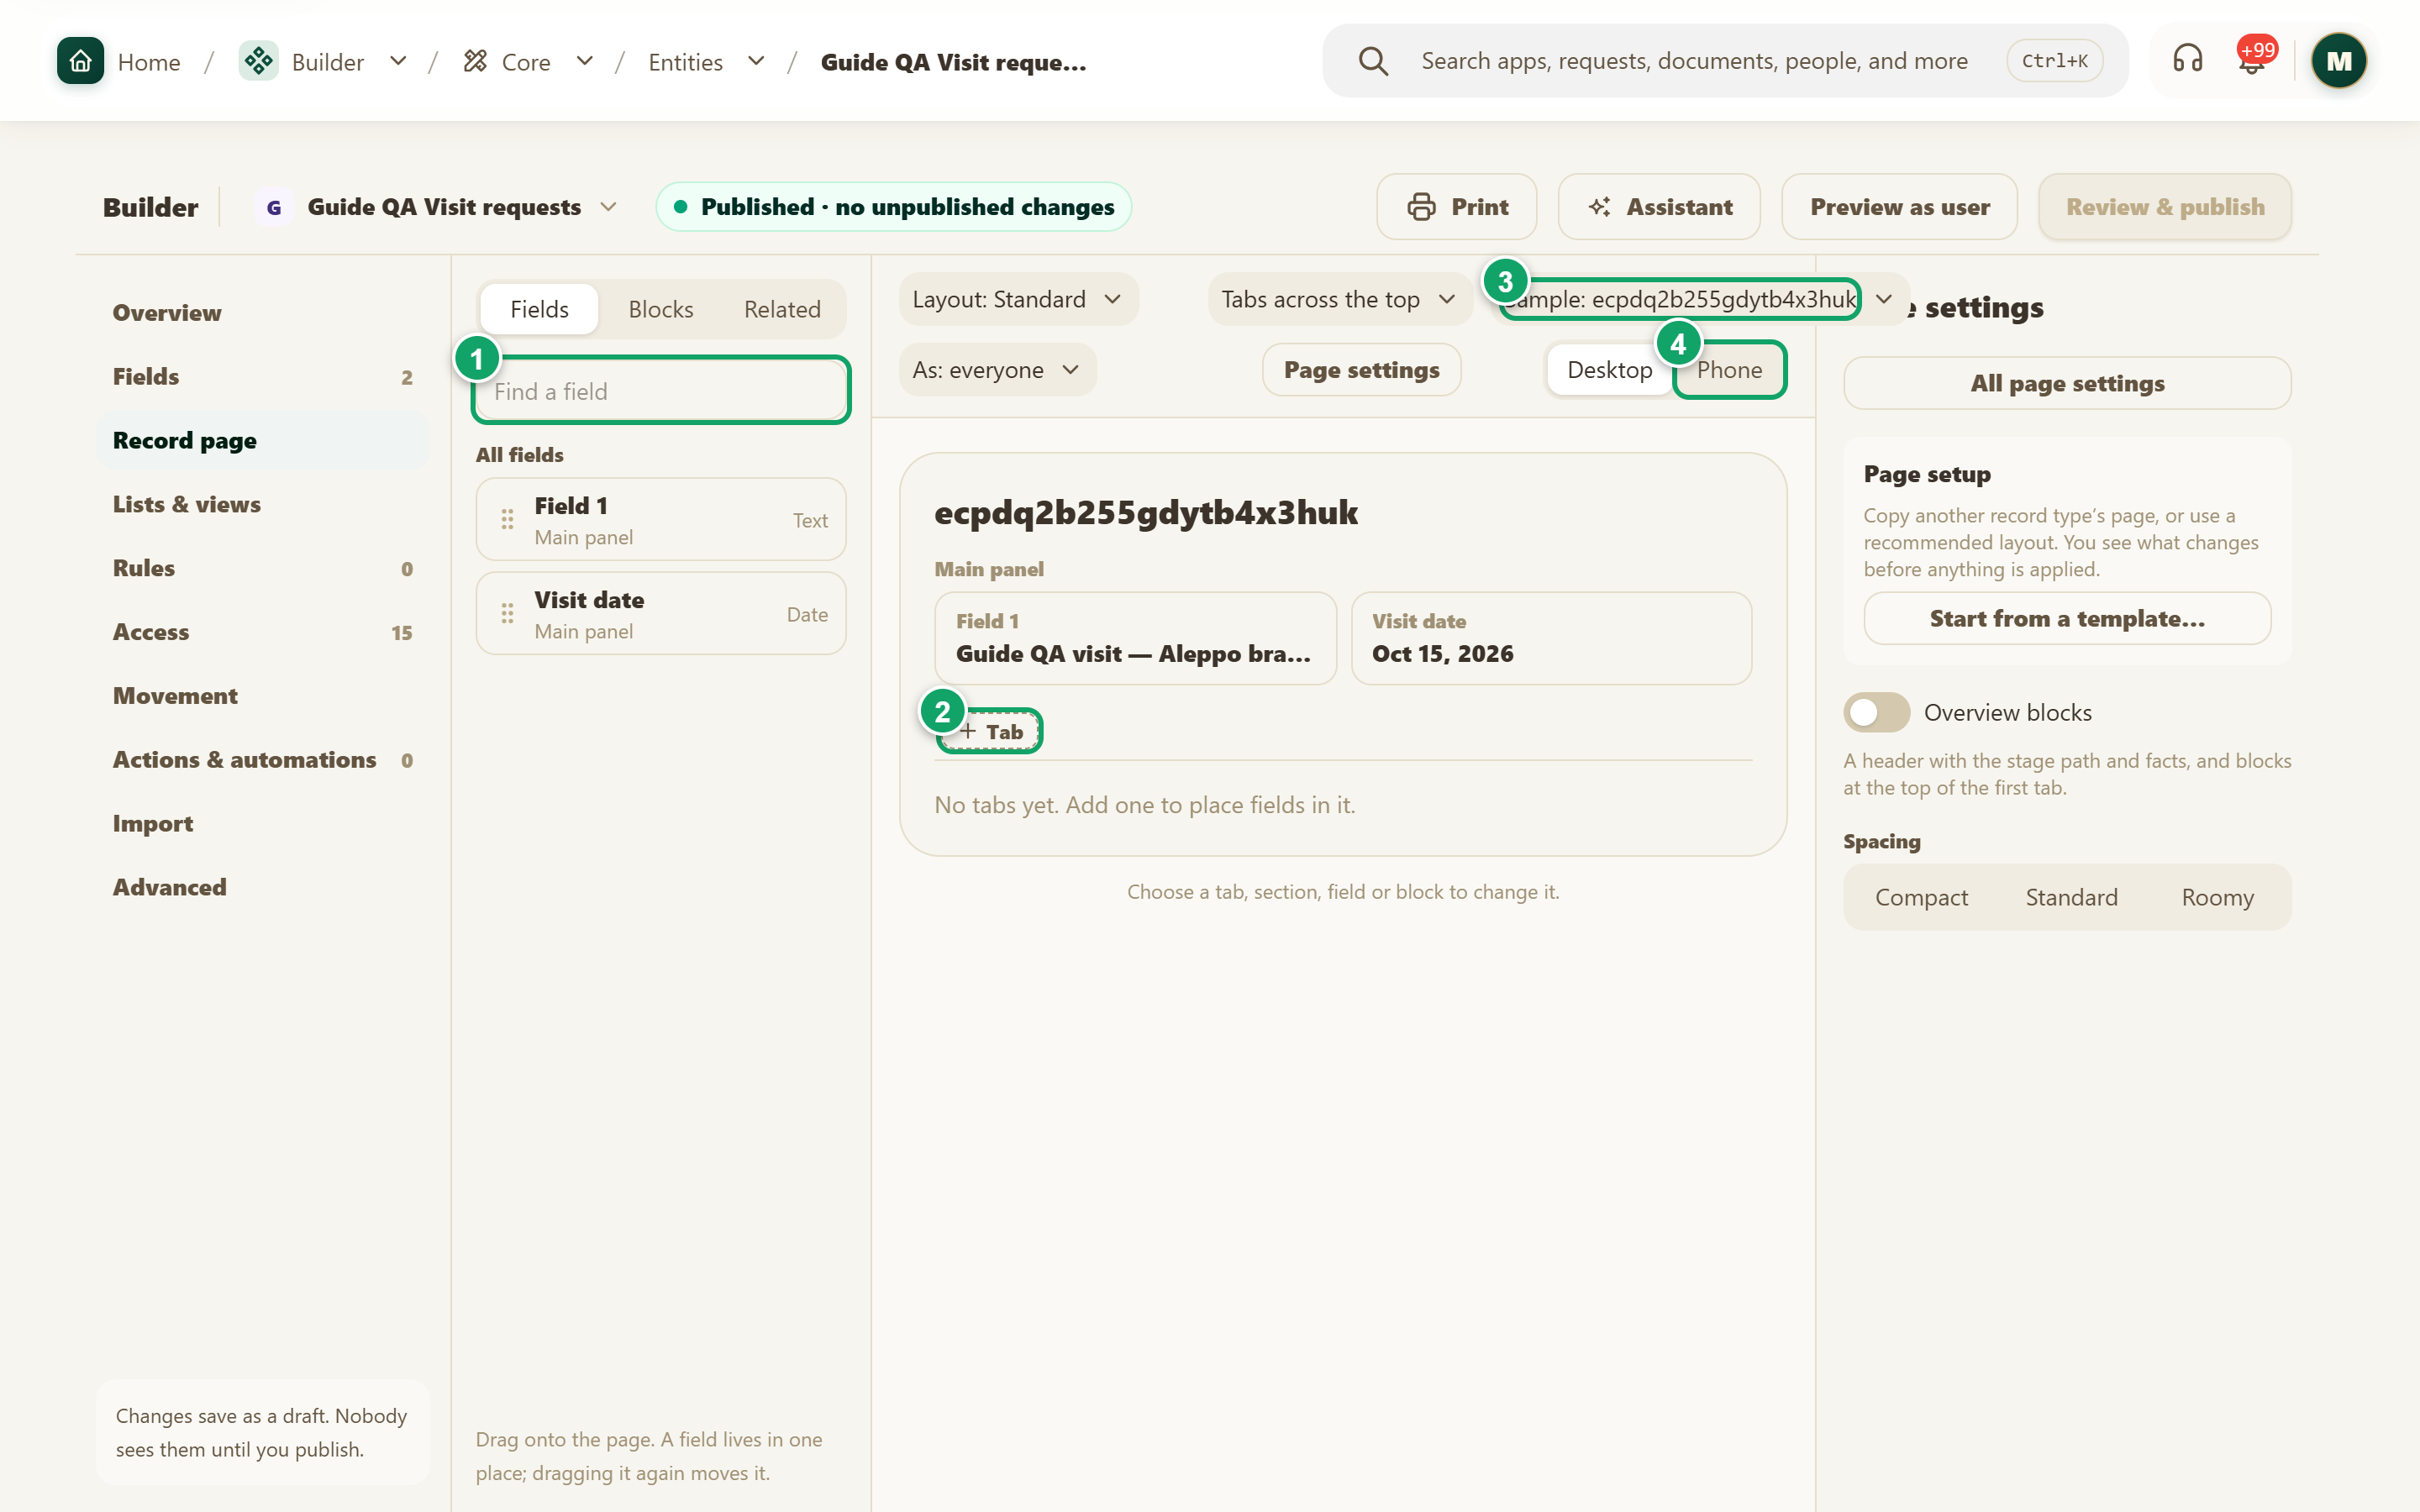
\includegraphics[width=0.95\linewidth,height=0.72\textheight,keepaspectratio]{figures/screens/ch06-ws-record-page-en.png}
\caption{The “Record page” section with a real record preview}
\label{fig:builder-record-page-screen}
\shotnote{The section shows the page parts on one side and the page itself in the middle with a test record’s values, so you see the arrangement before publishing. ① “Find a field”: finds the field you want to drag onto the page. ② “+ Tab”: adds a tab to hold sections and fields. ③ “Sample”: the record used to preview the page. ④ “Phone”: shows the page as it appears on a small screen.}
\end{figure}


\begin{table}[H]
\centering
\caption{What do you find here?}
\label{tab:builder-record-page-data}
\begin{tabularx}{\linewidth}{R{3.6cm} Y}
\rcHeaderRow
\thh{Section} & \thh{Content and action}\\
Tabs and sections & Create a “New tab” or “New section”, then drag fields into it. A field has one place on the page; dragging it again moves it.\\
Page parts & Groups “All fields”, “Blocks” and “Related” lists, and shows the fields that are “Not on the page yet”.\\
Layout and header & Chooses the page shape, tabs or a section list, with header settings and overview blocks.\\
Preview & Shows the page with a sample of a real record, as a chosen role sees it, on desktop or phone.\\
\end{tabularx}
\end{table}

\begin{figure}[H]
\centering
\begin{tikzpicture}[node distance=0.5cm]
\node[entity] (page) {Record page};
\node[entity,below=0.7cm of page] (tab) {Tab};
\node[entity,below=0.7cm of tab] (section) {Section};
\node[entity,below=0.7cm of section] (field) {Field};
\draw[dependsOn] (page) -- (tab);
\draw[dependsOn] (tab) -- (section);
\draw[dependsOn] (section) -- (field);
\end{tikzpicture}
\rclegend
\caption{How the page is arranged}
\label{fig:builder-record-page-tree}
\shotnote{The figure shows the levels of arrangement: the page holds tabs, each tab holds sections and each section holds fields. So you create the tab and section first and then drag fields into them; a field you place in no section is still saved but does not appear on the page.}
\end{figure}

\subsection{Steps and check}
\begin{enumerate}
\item Open the record type and choose “Record page”.
\item Create the tabs the work needs, then add one or more sections to each tab.
\item Drag each field from “Page parts” into the right section, and check “Not on the page yet” so no important field is left off the page.
\item Switch the preview size to “Phone” to make sure the page is clear on a small screen.
\end{enumerate}

\textbf{Check and recovery:} the preview should show the fields in the tabs and sections you chose. If a field does not appear, find it under “Not on the page yet” and drag it into a section; if a message says a field is placed in a tab that does not exist, move it to an existing tab.

\clearpage
\section{Lists \& views}
\label{sec:builder-feature-lists}

The “Lists \& views” section decides how the type's records appear together when a user opens the list. You choose the views people can switch between, such as “Table”, “Kanban” or “Calendar”, the visible columns and the figures that summarize the list at the top.

\textbf{Path and who uses it:} record type → “Lists \& views”. Used by whoever builds the type, and useful to everyone who follows the records daily.

\begin{rcnote}[Example: Horizon]
The system administrator shows visit requests in a “Table” with number, branch, date and status columns, and adds a “Calendar” by visit date, so Sarah Al-Khatib sees the week's visits at a glance. They start by turning on switch ① to choose the table and the calendar.
\end{rcnote}

\begin{figure}[H]
\centering
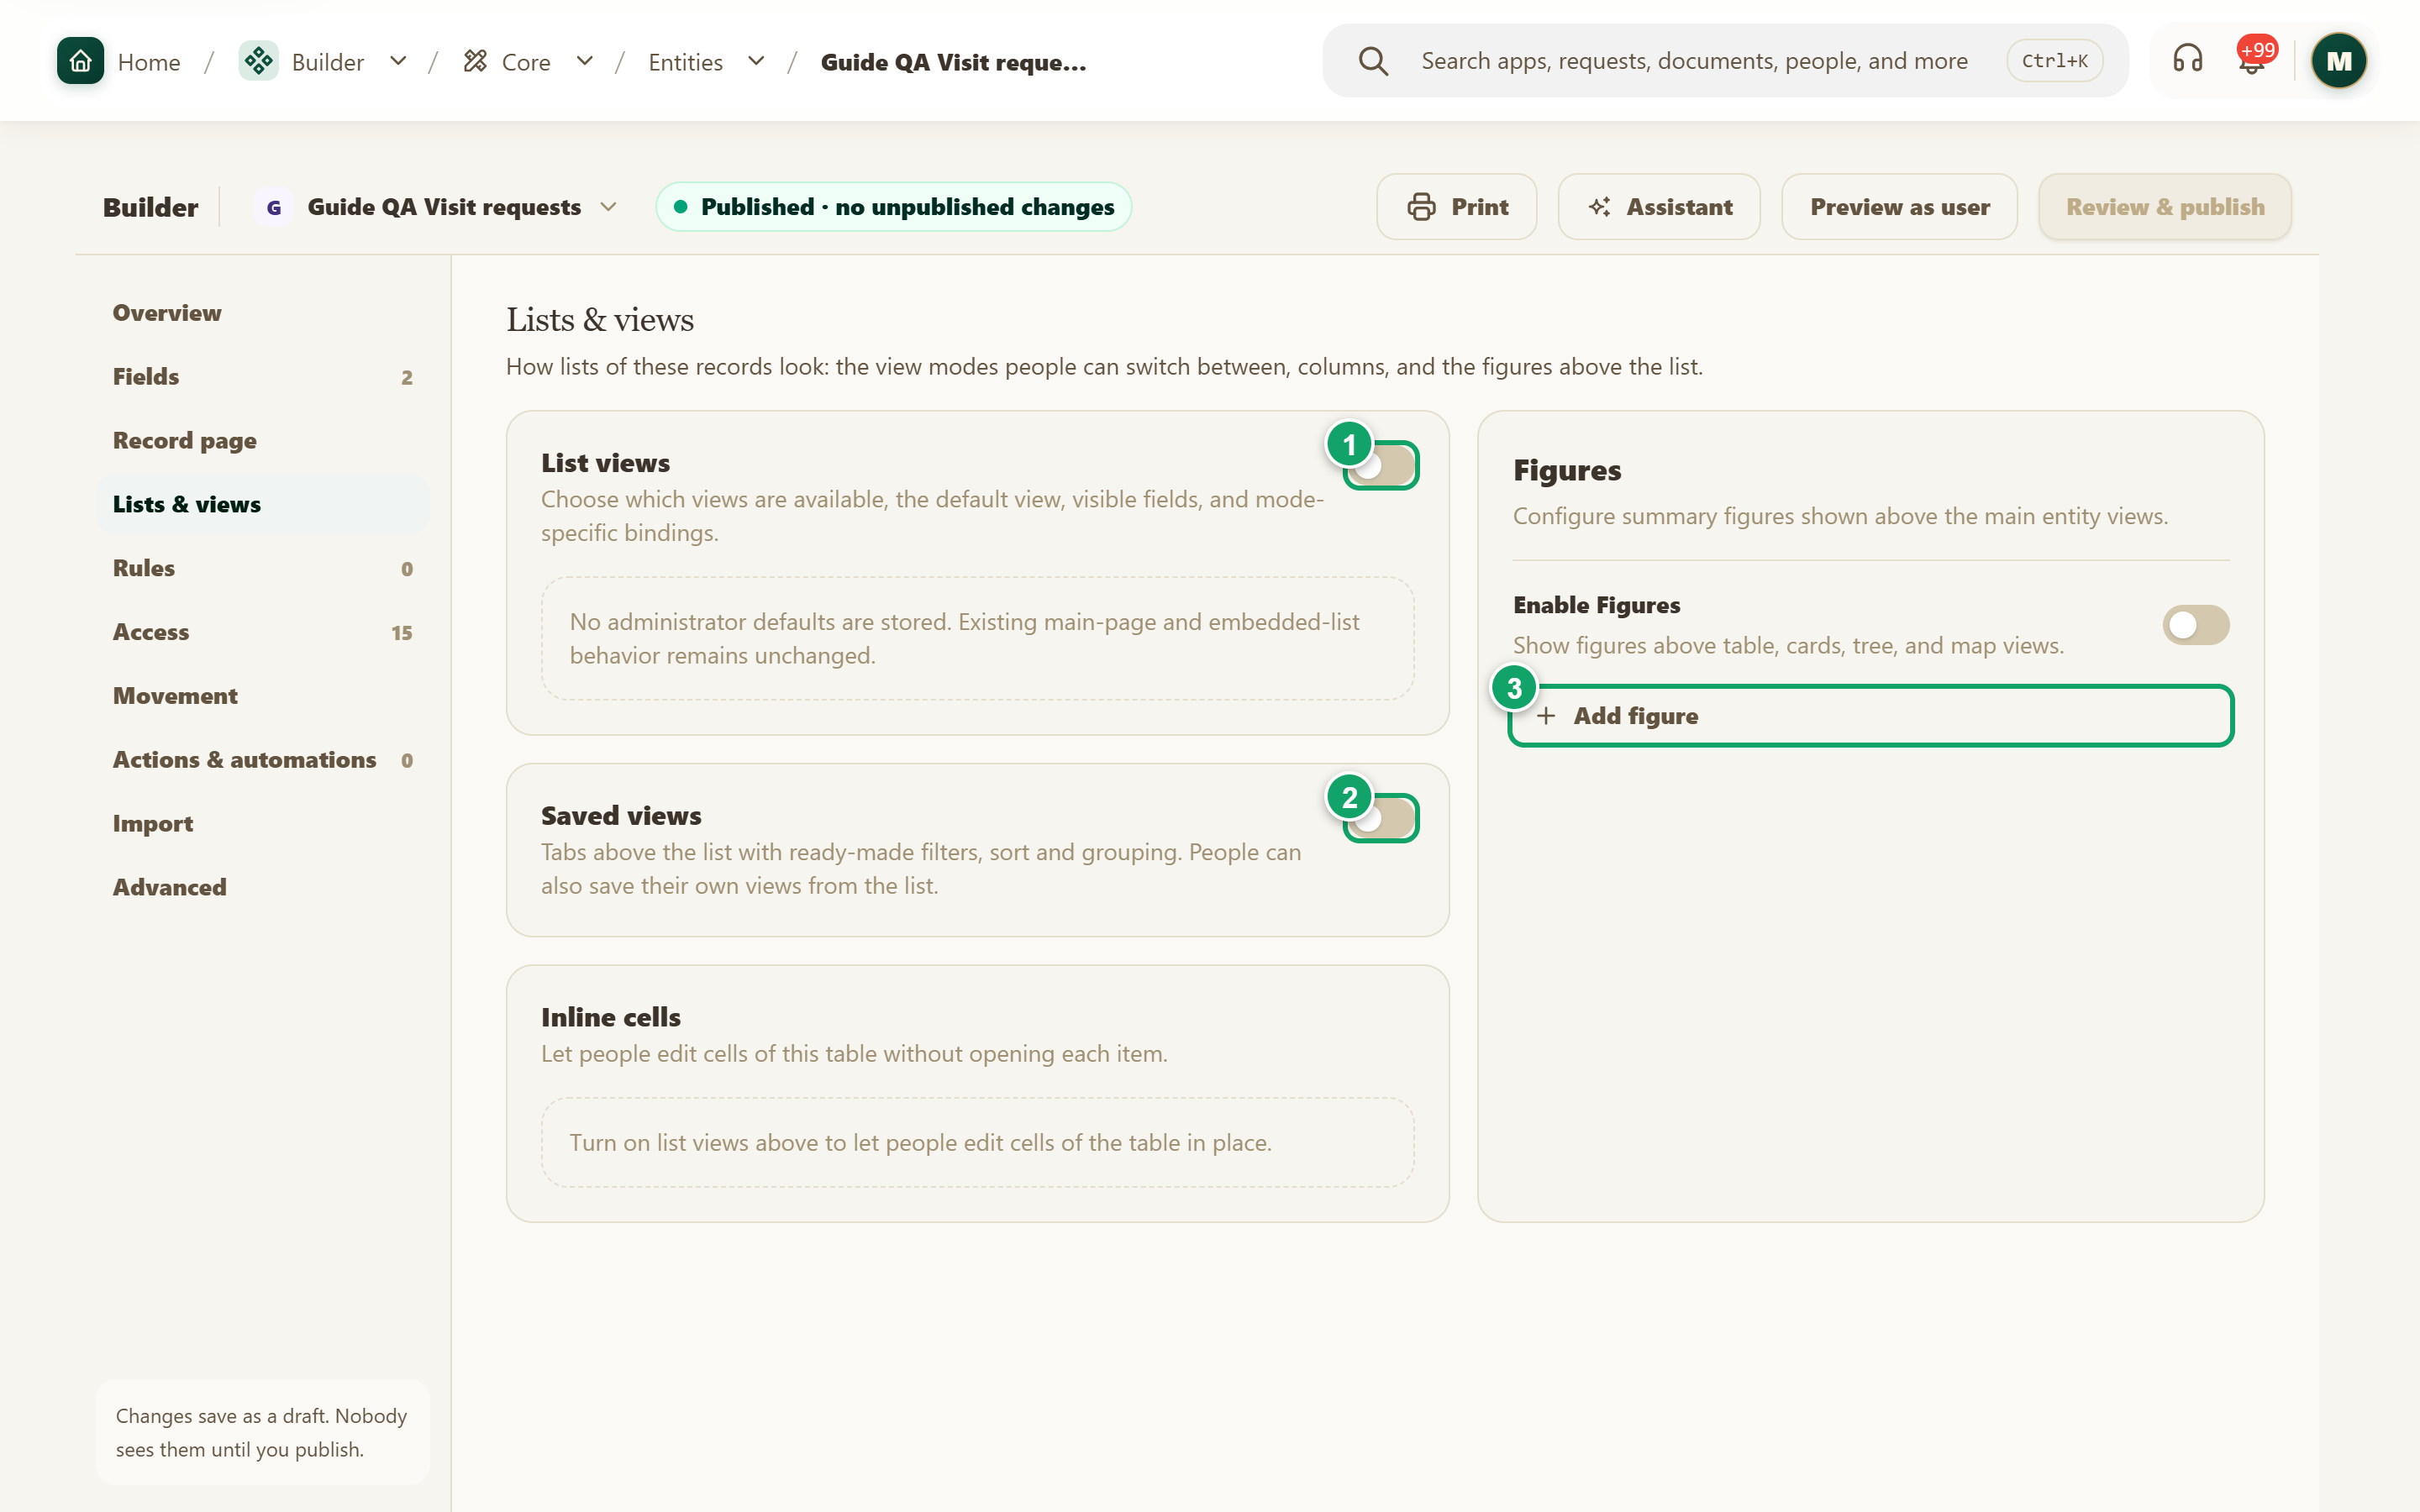
\includegraphics[width=0.95\linewidth,height=0.72\textheight,keepaspectratio]{figures/screens/ch06-ws-lists-en.png}
\caption{The “Lists \& views” section}
\label{fig:builder-lists-screen}
\shotnote{The section gathers what controls how the record list looks. All switches are off here, so the list uses its default setup. ① The “List views” switch: lets you choose the available and default views and the columns. ② The “Saved views” switch: adds ready-made tabs above the list. ③ “Add figure”: adds a summary number above the list.}
\end{figure}

\begin{figure}[H]
\centering
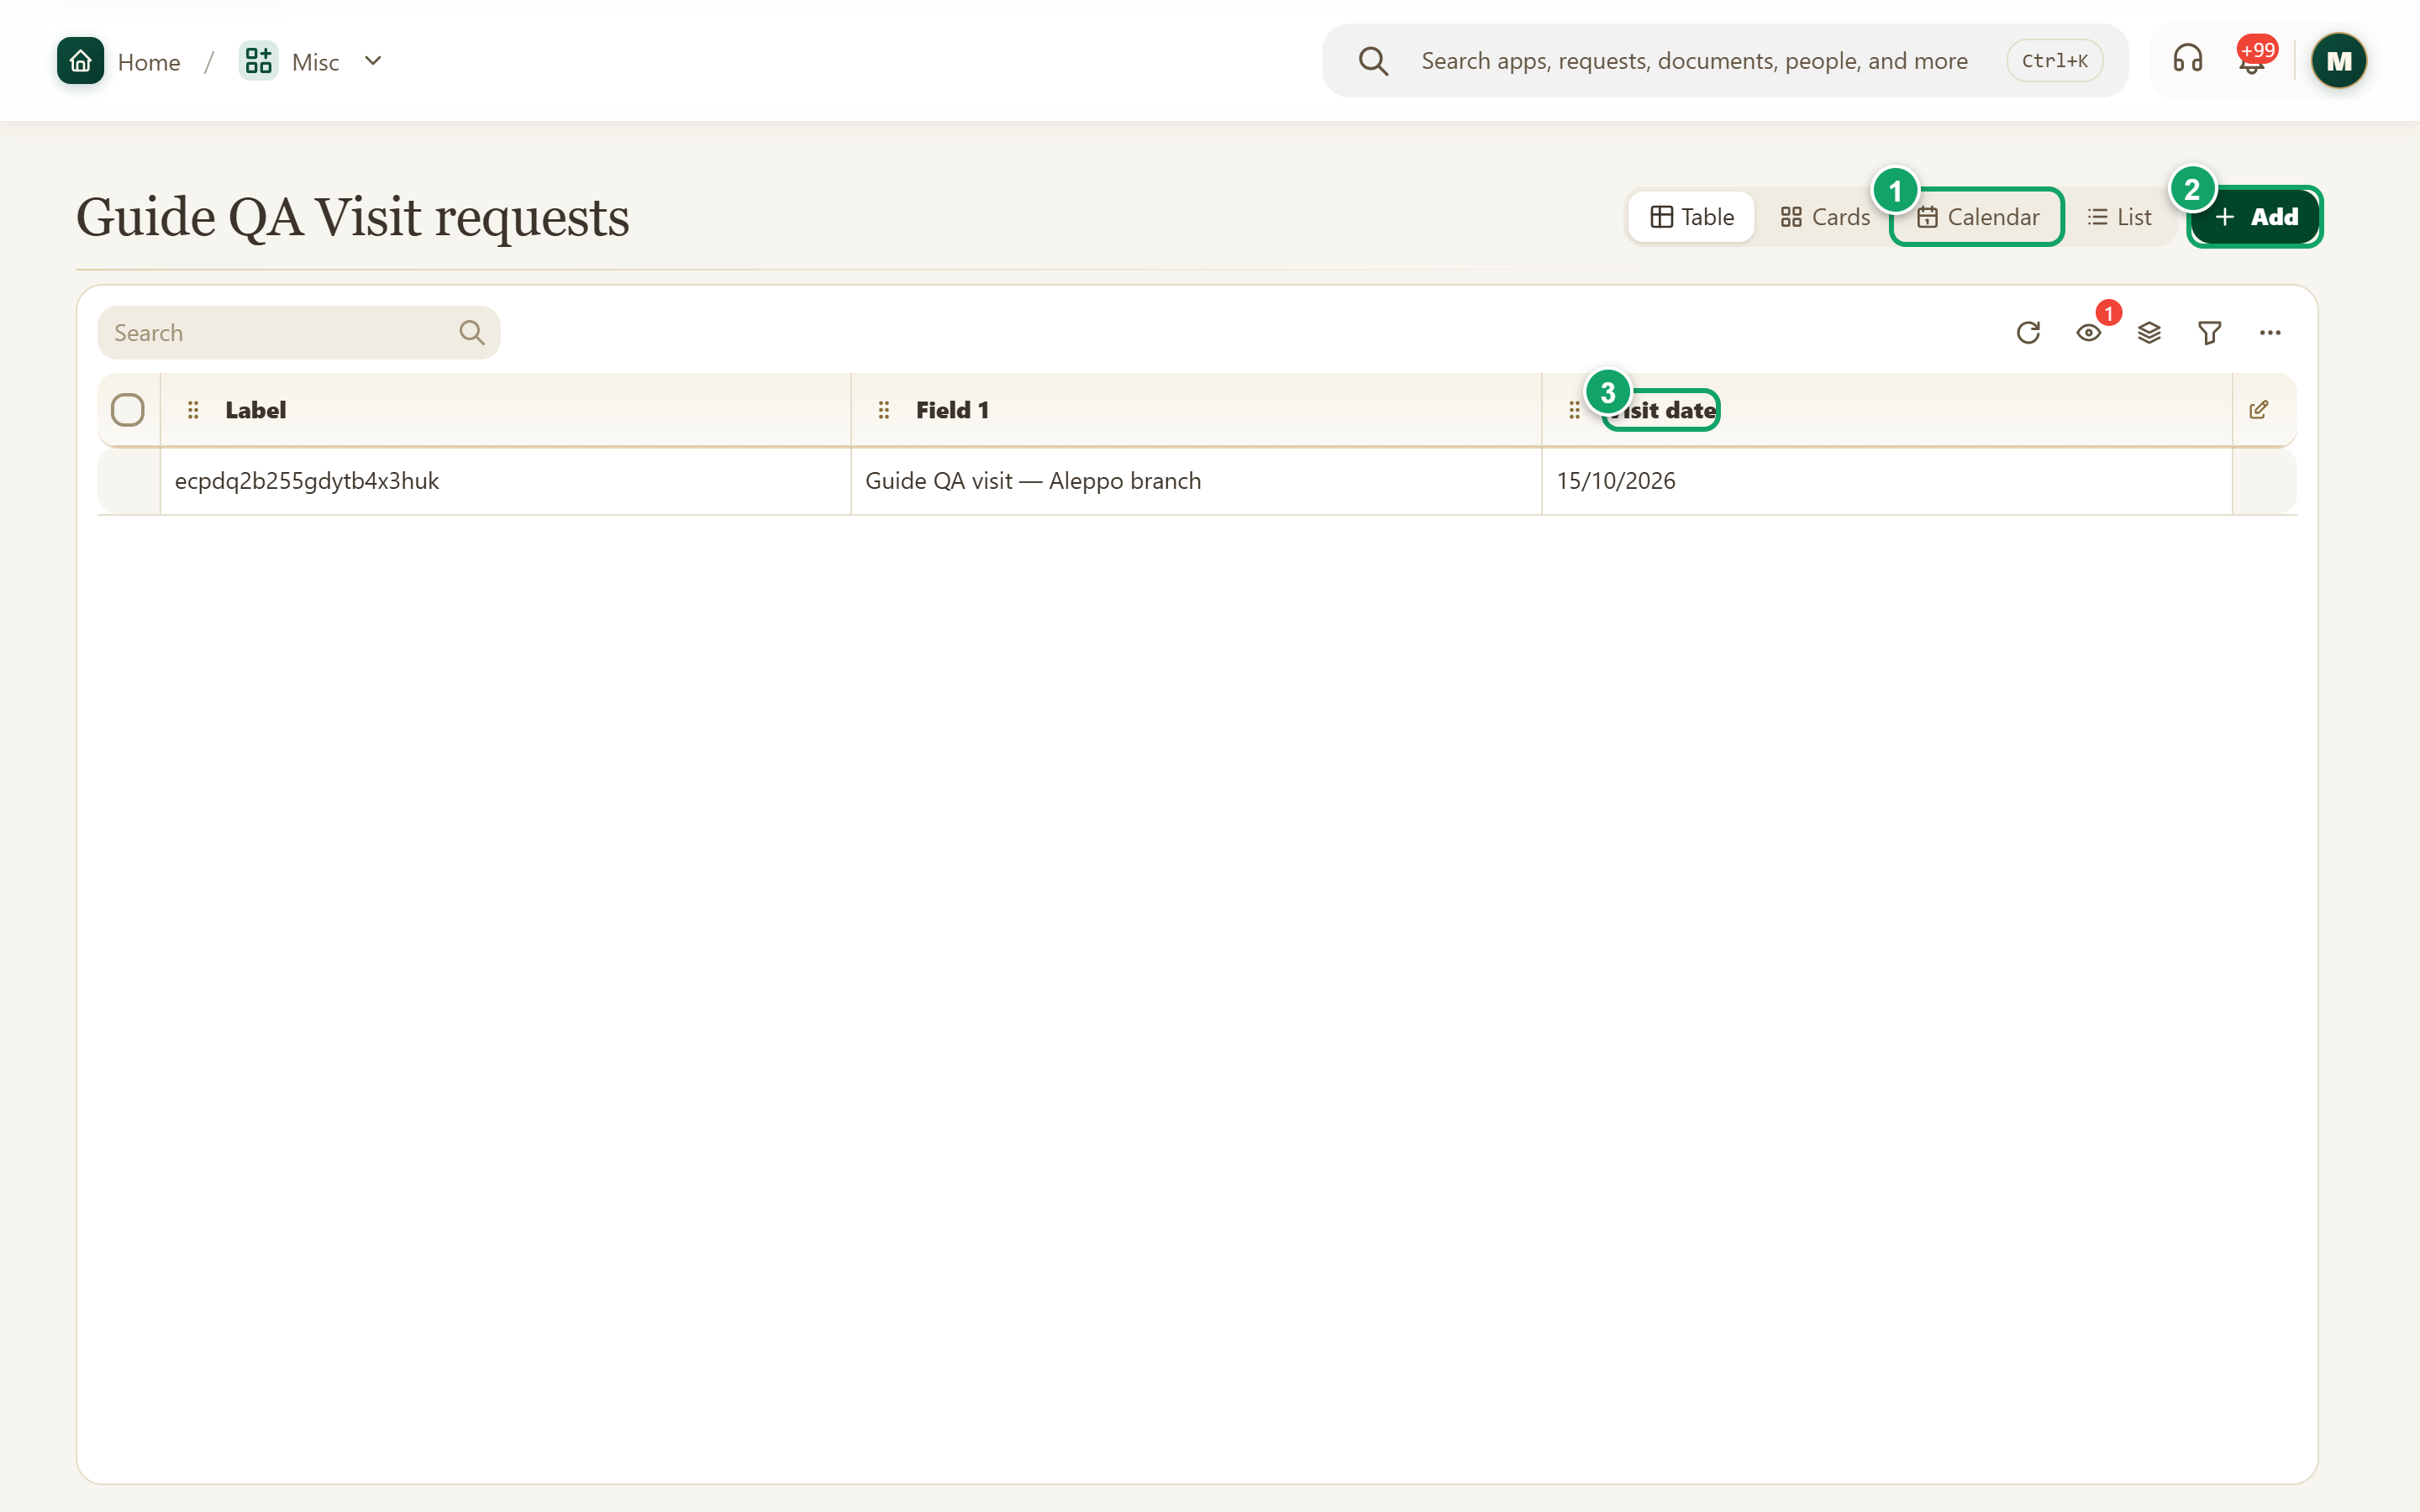
\includegraphics[width=0.95\linewidth,height=0.72\textheight,keepaspectratio]{figures/screens/ch06-records-en.png}
\caption{The type’s record list after publishing}
\label{fig:builder-lists-records}
\shotnote{This is the list users see after publishing, with a test record created on test2 and reopened to confirm it saved. ① “Calendar”: this view appeared because the type has a date field. ② “Add”: creates a new record. ③ The “Visit date” column: shows the test record’s saved value after it was reopened.}
\end{figure}


\begin{table}[H]
\centering
\caption{Available views}
\label{tab:builder-lists-modes}
\begin{tabularx}{\linewidth}{R{3.6cm} Y}
\rcHeaderRow
\thh{View} & \thh{When it fits}\\
Table and List & Always available for reviewing and comparing records row by row, with sorting and filtering.\\
Cards and Gallery & “Cards” is always available; “Gallery” appears when the type has an image field.\\
Kanban & Spreads records into columns by status or a select value, and appears when a suitable field exists.\\
Calendar and Timeline & Appear when the type has a date or time-range field, such as appointments and stages.\\
Map & Appears when the type has a “Location” or “Boundary” field.\\
Tree & Appears when you turn on “Parent records” in “Advanced”, showing records as parents and children.\\
\end{tabularx}
\end{table}

\begin{figure}[H]
\centering
\begin{tikzpicture}[node distance=0.5cm]
\node[entity] (fields) {Fields};
\node[entityOpt,below right=0.7cm and 0.3cm of fields] (cal) {Calendar};
\node[entityOpt,below left=0.7cm and 0.3cm of fields] (map) {Map};
\draw[dependsOnOpt] (fields.south) -- ++(0,-0.3) -| (cal.north);
\draw[dependsOnOpt] (fields.south) -- ++(0,-0.3) -| (map.north);
\end{tikzpicture}
\rclegend
\caption{Views that depend on the field type}
\label{fig:builder-lists-depends}
\shotnote{The figure shows that some views need a field of a certain type: the calendar needs a date, and the map needs a location or boundary. So if a view you want is missing, check the fields first, because the view does not appear among the options without the field it relies on.}
\end{figure}

\subsection{Steps and check}
\begin{enumerate}
\item Open the record type and choose “Lists \& views”.
\item Turn on the views the team needs, and choose the default view that opens first.
\item Choose the visible columns, order them by importance for daily work, and add summary figures when needed.
\end{enumerate}

\textbf{Check and recovery:} “Overview” should show the default view and the number of saved views. After publishing, open the record list and switch between views to confirm them; if a view is empty, check that the records have a value in the field it relies on.

\clearpage
\section{Rules}
\label{sec:builder-feature-rules}

A rule makes a record behave according to its values, without the user having to remember it. It can show a field when a certain value is chosen, lock it after creation, make it required in a given situation, or refuse an illogical value. The “Rules” section gathers all of these rules in one list.

\textbf{Path and who uses it:} record type → “Rules”. Used by whoever builds the type, once the fields are complete.

\begin{rcnote}[Example: Horizon]
The system administrator adds a rule that shows the “Rejection reason” field only when the status is “Rejected”, and a rule that checks the visit date is on or after the request date. They add both rules from ①.
\end{rcnote}

\begin{figure}[H]
\centering
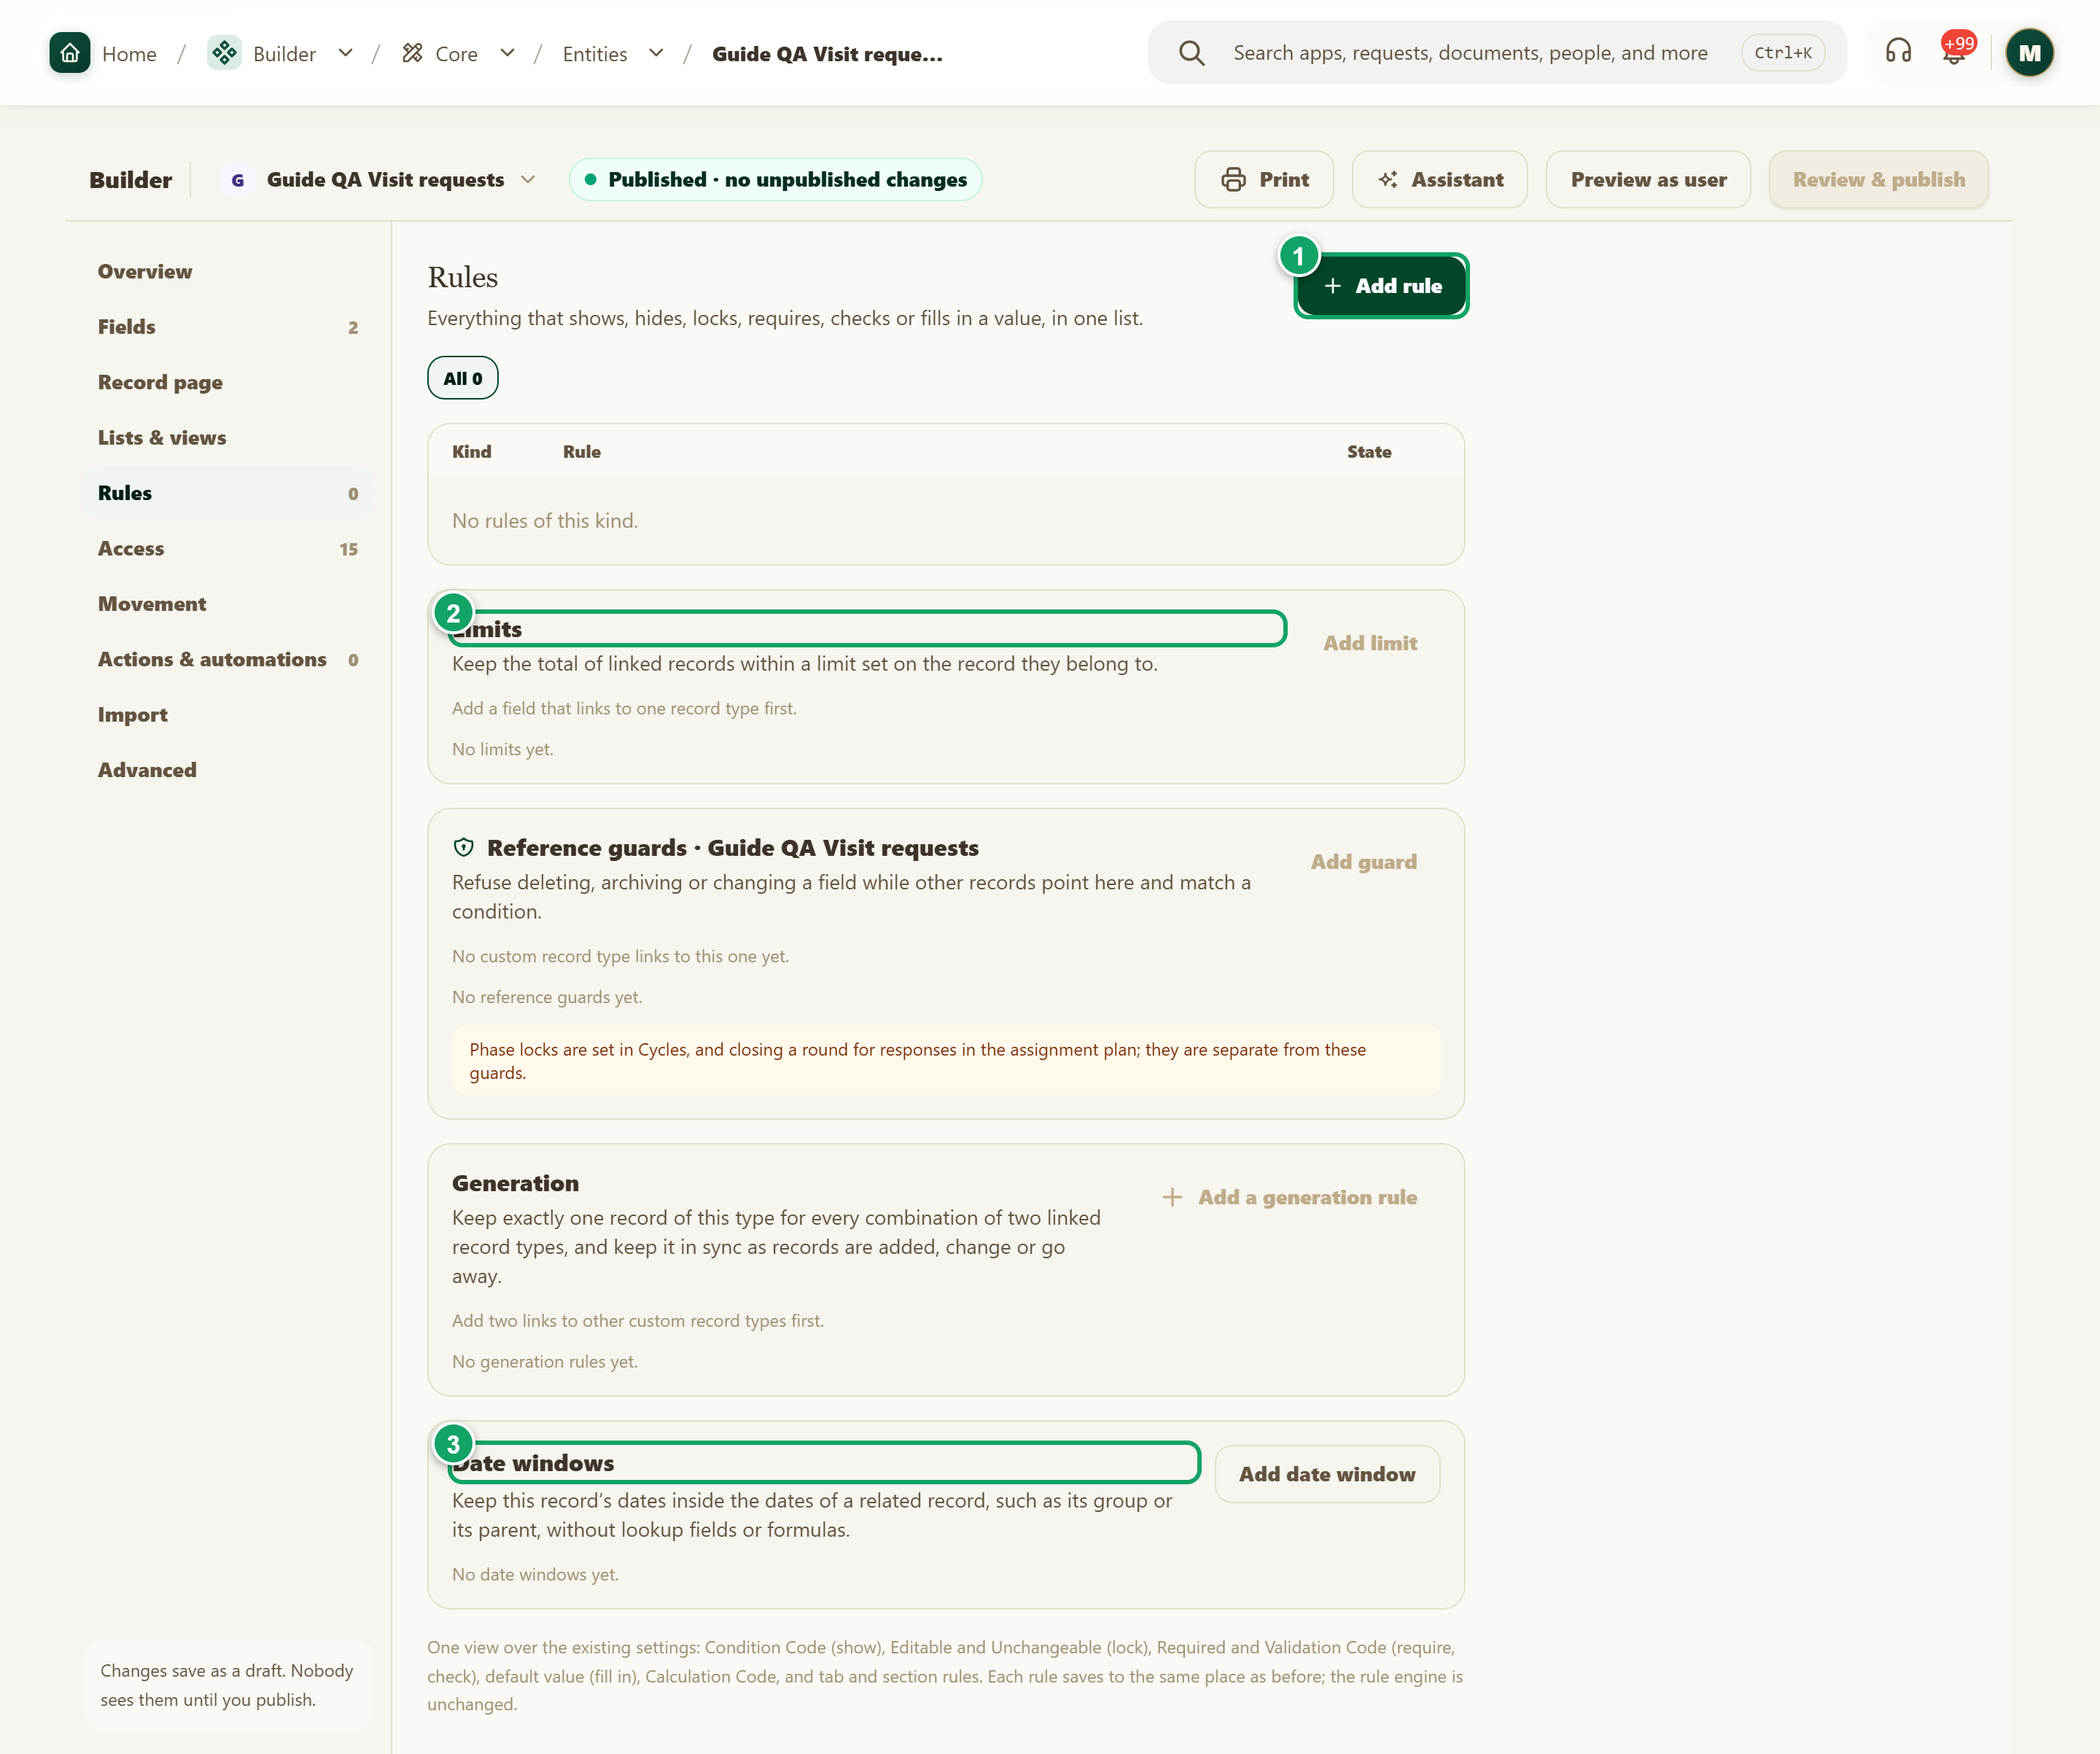
\includegraphics[width=0.95\linewidth,height=0.72\textheight,keepaspectratio]{figures/screens/ch06-ws-rules-en.png}
\caption{The “Rules” section and its extra tools}
\label{fig:builder-rules-screen}
\shotnote{The rules list sits at the top of the section, with other data-protecting tools below it, such as limits and date windows. The list is empty because the test type has no rules. ① “Add rule”: opens the rule editor. ② “Limits”: keeps the total of linked records within a limit. ③ “Date windows”: keeps the record’s dates inside a related record’s dates.}
\end{figure}


\begin{table}[H]
\centering
\caption{Rule kinds}
\label{tab:builder-rules-kinds}
\begin{tabularx}{\linewidth}{R{3.6cm} Y}
\rcHeaderRow
\thh{Kind} & \thh{What does it do?}\\
Show or hide & Shows a field, tab or section when a condition is met and hides it otherwise.\\
Lock editing & Prevents changes to a field, tab or section: “Locked when” a condition is met, “Editable only when”, or “After creation”.\\
Require & Makes the field required “Always” or “Only when…” a condition is met, with a message explaining why.\\
Check value & Refuses the value unless it is, for example, more than a number, after a date or different from another field, and shows your message.\\
Fill in value & Starts the field with a ready value the user can change.\\
Calculate & Lists calculated fields; you edit them in the “Fields” section.\\
\end{tabularx}
\end{table}

\begin{table}[H]
\centering
\caption{Other rules that live elsewhere}
\label{tab:builder-rules-other}
\begin{tabularx}{\linewidth}{R{3.6cm} Y}
\rcHeaderRow
\thh{Rule} & \thh{Where do you find it?}\\
Limits & Under the rules list: keeps the total or count of linked records within a limit, then refuses the excess or warns and asks for a reason.\\
Lifecycle rules & On the “Status” field in “Fields”: for each status you decide whether the record is “Locked” or “Locked except…”, and you can “Block delete”. Needs a fixed status template.\\
Unique values & In “Advanced”: prevents two records from sharing a code or a combination of values.\\
\end{tabularx}
\end{table}

\begin{figure}[H]
\centering
\begin{tikzpicture}[node distance=0.5cm]
\node[stepBox] (a) {Choose the rule kind};
\node[stepBox,below=of a] (b) {Condition: When…};
\node[stepBox,below=of b] (c) {Target: field, tab or section};
\node[stepBox,below=of c] (d) {Try it, then save to draft};
\draw[flowsTo] (a) -- (b);
\draw[flowsTo] (b) -- (c);
\draw[flowsTo] (c) -- (d);
\end{tikzpicture}
\rclegend
\caption{How a rule is built}
\label{fig:builder-rules-flow}
\shotnote{A rule reads like a sentence: “When” a condition is met, apply an effect to a chosen target. The diagram puts the test before saving, because “Try it” runs the rule on sample records and exposes a wrong condition before it reaches users. Rules apply to everyone who can edit the record, so they are not a way to treat one role differently from another.}
\end{figure}

\subsection{Steps and check}
\begin{enumerate}
\item Open the record type, choose “Rules”, then press “Add rule”.
\item Choose the rule kind, then build the condition under “When”, joining conditions with “+ And” or “+ Or”.
\item Pick the target from “Choose a field, tab or section”, and write the “Message people see” when needed.
\item Press “Try it” and review the result on the samples, then press “Save to draft”.
\end{enumerate}

\textbf{Check and recovery:} the rule should appear in the table with the state “OK”. If it shows “Broken”, open it and fix the field or condition that changed. If you want only some roles to see a field, use “Access”, not “Rules”.

\clearpage
\section{Access}
\label{sec:builder-feature-access}

Access decides who can do what with the records of this type. These actions are called “verbs”, such as seeing records in lists, opening, adding, changing and deleting them. The “Access” section shows roles and verbs in one grid, and it edits the same roles as Settings › Roles, so it does not create a second permission system.

\textbf{Path and who uses it:} record type → “Access”. Used by whoever builds the type and holds the right to update roles.

\begin{rcnote}[Example: Horizon]
The system administrator gives branch coordinators, including Omar Haddad, the create and open verbs on “Visit requests”, and gives the HR Manager Sarah Al-Khatib the update verb so she can record her decision. Then they confirm Omar’s access with tool ③.
\end{rcnote}

\begin{figure}[H]
\centering
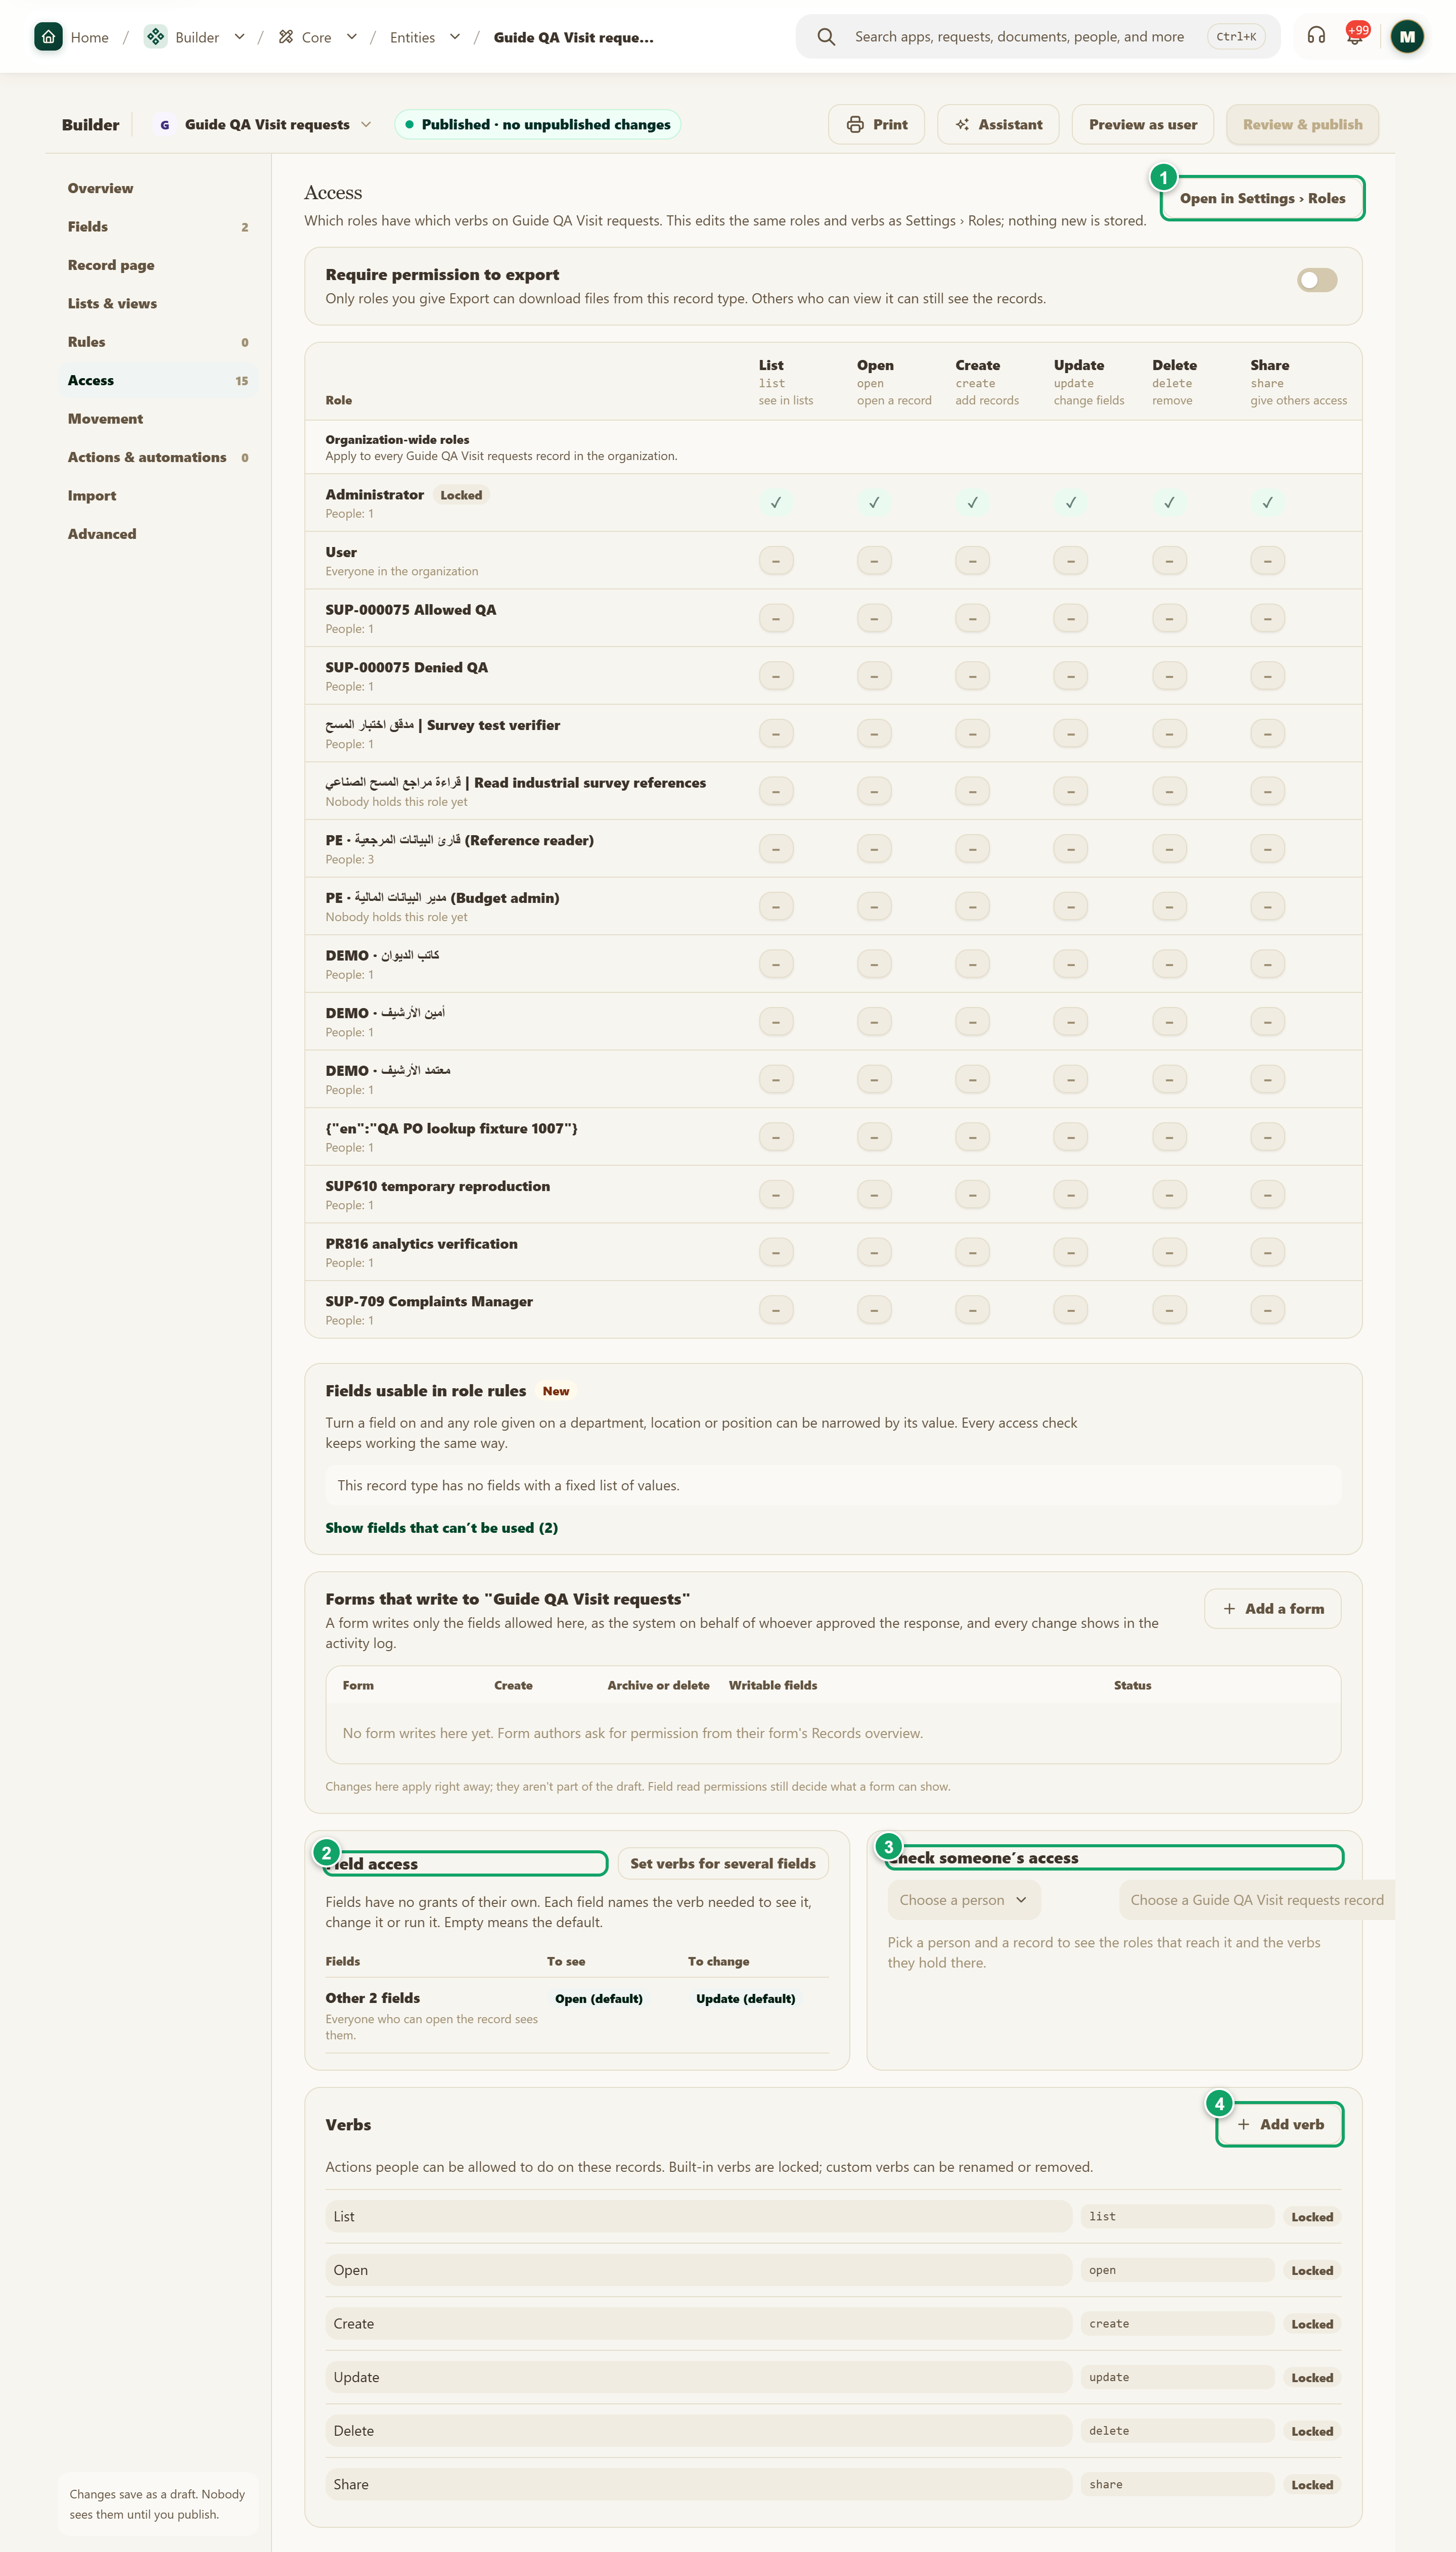
\includegraphics[width=0.95\linewidth,height=0.72\textheight,keepaspectratio]{figures/screens/ch06-ws-access-en.png}
\caption{The “Access” section}
\label{fig:builder-access-screen}
\shotnote{The section shows roles and verbs on this type, then field access, an access check tool and the verbs list. The roles shown are the test organization’s roles. ① “Open in Settings › Roles”: opens the same roles in settings. ② “Field access”: sets the verb needed to see or change a field. ③ “Check someone’s access”: shows what a person can do on a record. ④ “Add verb”: adds a custom verb such as approval.}
\end{figure}


\begin{table}[H]
\centering
\caption{Built-in verbs}
\label{tab:builder-access-verbs}
\begin{tabularx}{\linewidth}{R{3.6cm} Y}
\rcHeaderRow
\thh{Verb} & \thh{What does it allow?}\\
\en{list} & See in lists.\\
\en{open} & Open a record.\\
\en{create} & Add records.\\
\en{update} & Change fields.\\
\en{delete} & Remove.\\
\en{share} & Give others access.\\
\en{export} & Download a file; it appears when “Require permission to export” is on.\\
\end{tabularx}
\end{table}

\begin{table}[H]
\centering
\caption{What do you find here?}
\label{tab:builder-access-data}
\begin{tabularx}{\linewidth}{R{3.6cm} Y}
\rcHeaderRow
\thh{Card} & \thh{Content and action}\\
Roles and verbs & Press a cell to grant a verb to a role or take it away. It shows organization-wide roles, roles on one record, and other roles with grants here.\\
Field access & Fields have no grants of their own; each field names the verb needed “To see”, “To change” or “To run” it. Empty means the default.\\
Verbs & “Add verb” for a custom verb, such as “Approve budget”, then grant it to roles.\\
Fields usable in role rules & Let a role be narrowed by a field's value, such as the branch.\\
Forms that write to this type & Decides which forms may write this type's fields. Changes here apply right away; they are not part of the draft.\\
Check someone's access & Pick a person and a record to see the roles that reach it and the verbs they hold.\\
\end{tabularx}
\end{table}

\begin{figure}[H]
\centering
\begin{tikzpicture}[node distance=0.5cm]
\node[entity] (role) {Role};
\node[entity,below=0.7cm of role] (verb) {Verb};
\node[entityOpt,below right=0.7cm and 0.3cm of verb] (field) {Field that needs the verb};
\node[entityOpt,below left=0.7cm and 0.3cm of verb] (records) {Records of the type};
\draw[dependsOn] (role) -- (verb);
\draw[dependsOnOpt] (verb.south) -- ++(0,-0.3) -| (field.north);
\draw[dependsOnOpt] (verb.south) -- ++(0,-0.3) -| (records.north);
\end{tikzpicture}
\rclegend
\caption{From role to what a person can do}
\label{fig:builder-access-model}
\shotnote{The figure shows that a person does not receive a permission directly but through their role, and the role holds verbs on the type's records. A sensitive field can ask for a specific verb, so only those holding it can see or change it. Start with the built-in verbs, and add a custom verb only for work that has its own meaning, such as approval.}
\end{figure}

\subsection{Steps and check}
\begin{enumerate}
\item Open the record type, choose “Access”, and review the roles shown.
\item Press the cells to give each role only the verbs its work needs.
\item For sensitive fields, open “Field access” and set the verb needed to see or change them.
\item Use “Check someone's access” on an employee and a test record, then publish the changes.
\end{enumerate}

\textbf{Check and recovery:} the check tool should show the expected verbs for the person, and after publishing the user should see only what concerns them. If the message “You need the Update verb on roles to change grants.” appears, ask the organization administrator; if a field does not appear for a user, review the verb it needs under “Field access”.

\clearpage
\section{Actions \& automations}
\label{sec:builder-feature-actions}

An action is a button on the record that creates a Word document or a spreadsheet from the record's data, opens a link, or starts a workflow. This section gathers the type's buttons and shows the automations linked to it and the calculated fields the system recalculates on a schedule.

\textbf{Path and who uses it:} record type → “Actions \& automations”. Used by whoever builds the type, after preparing the template or workflow the button will call.

\begin{rcnote}[Example: Horizon]
The system administrator adds a “Word document” button to the visit request that creates the visit confirmation letter from the request's data, and makes it available only to those holding the approval verb. The button starts from ①.
\end{rcnote}

\begin{figure}[H]
\centering
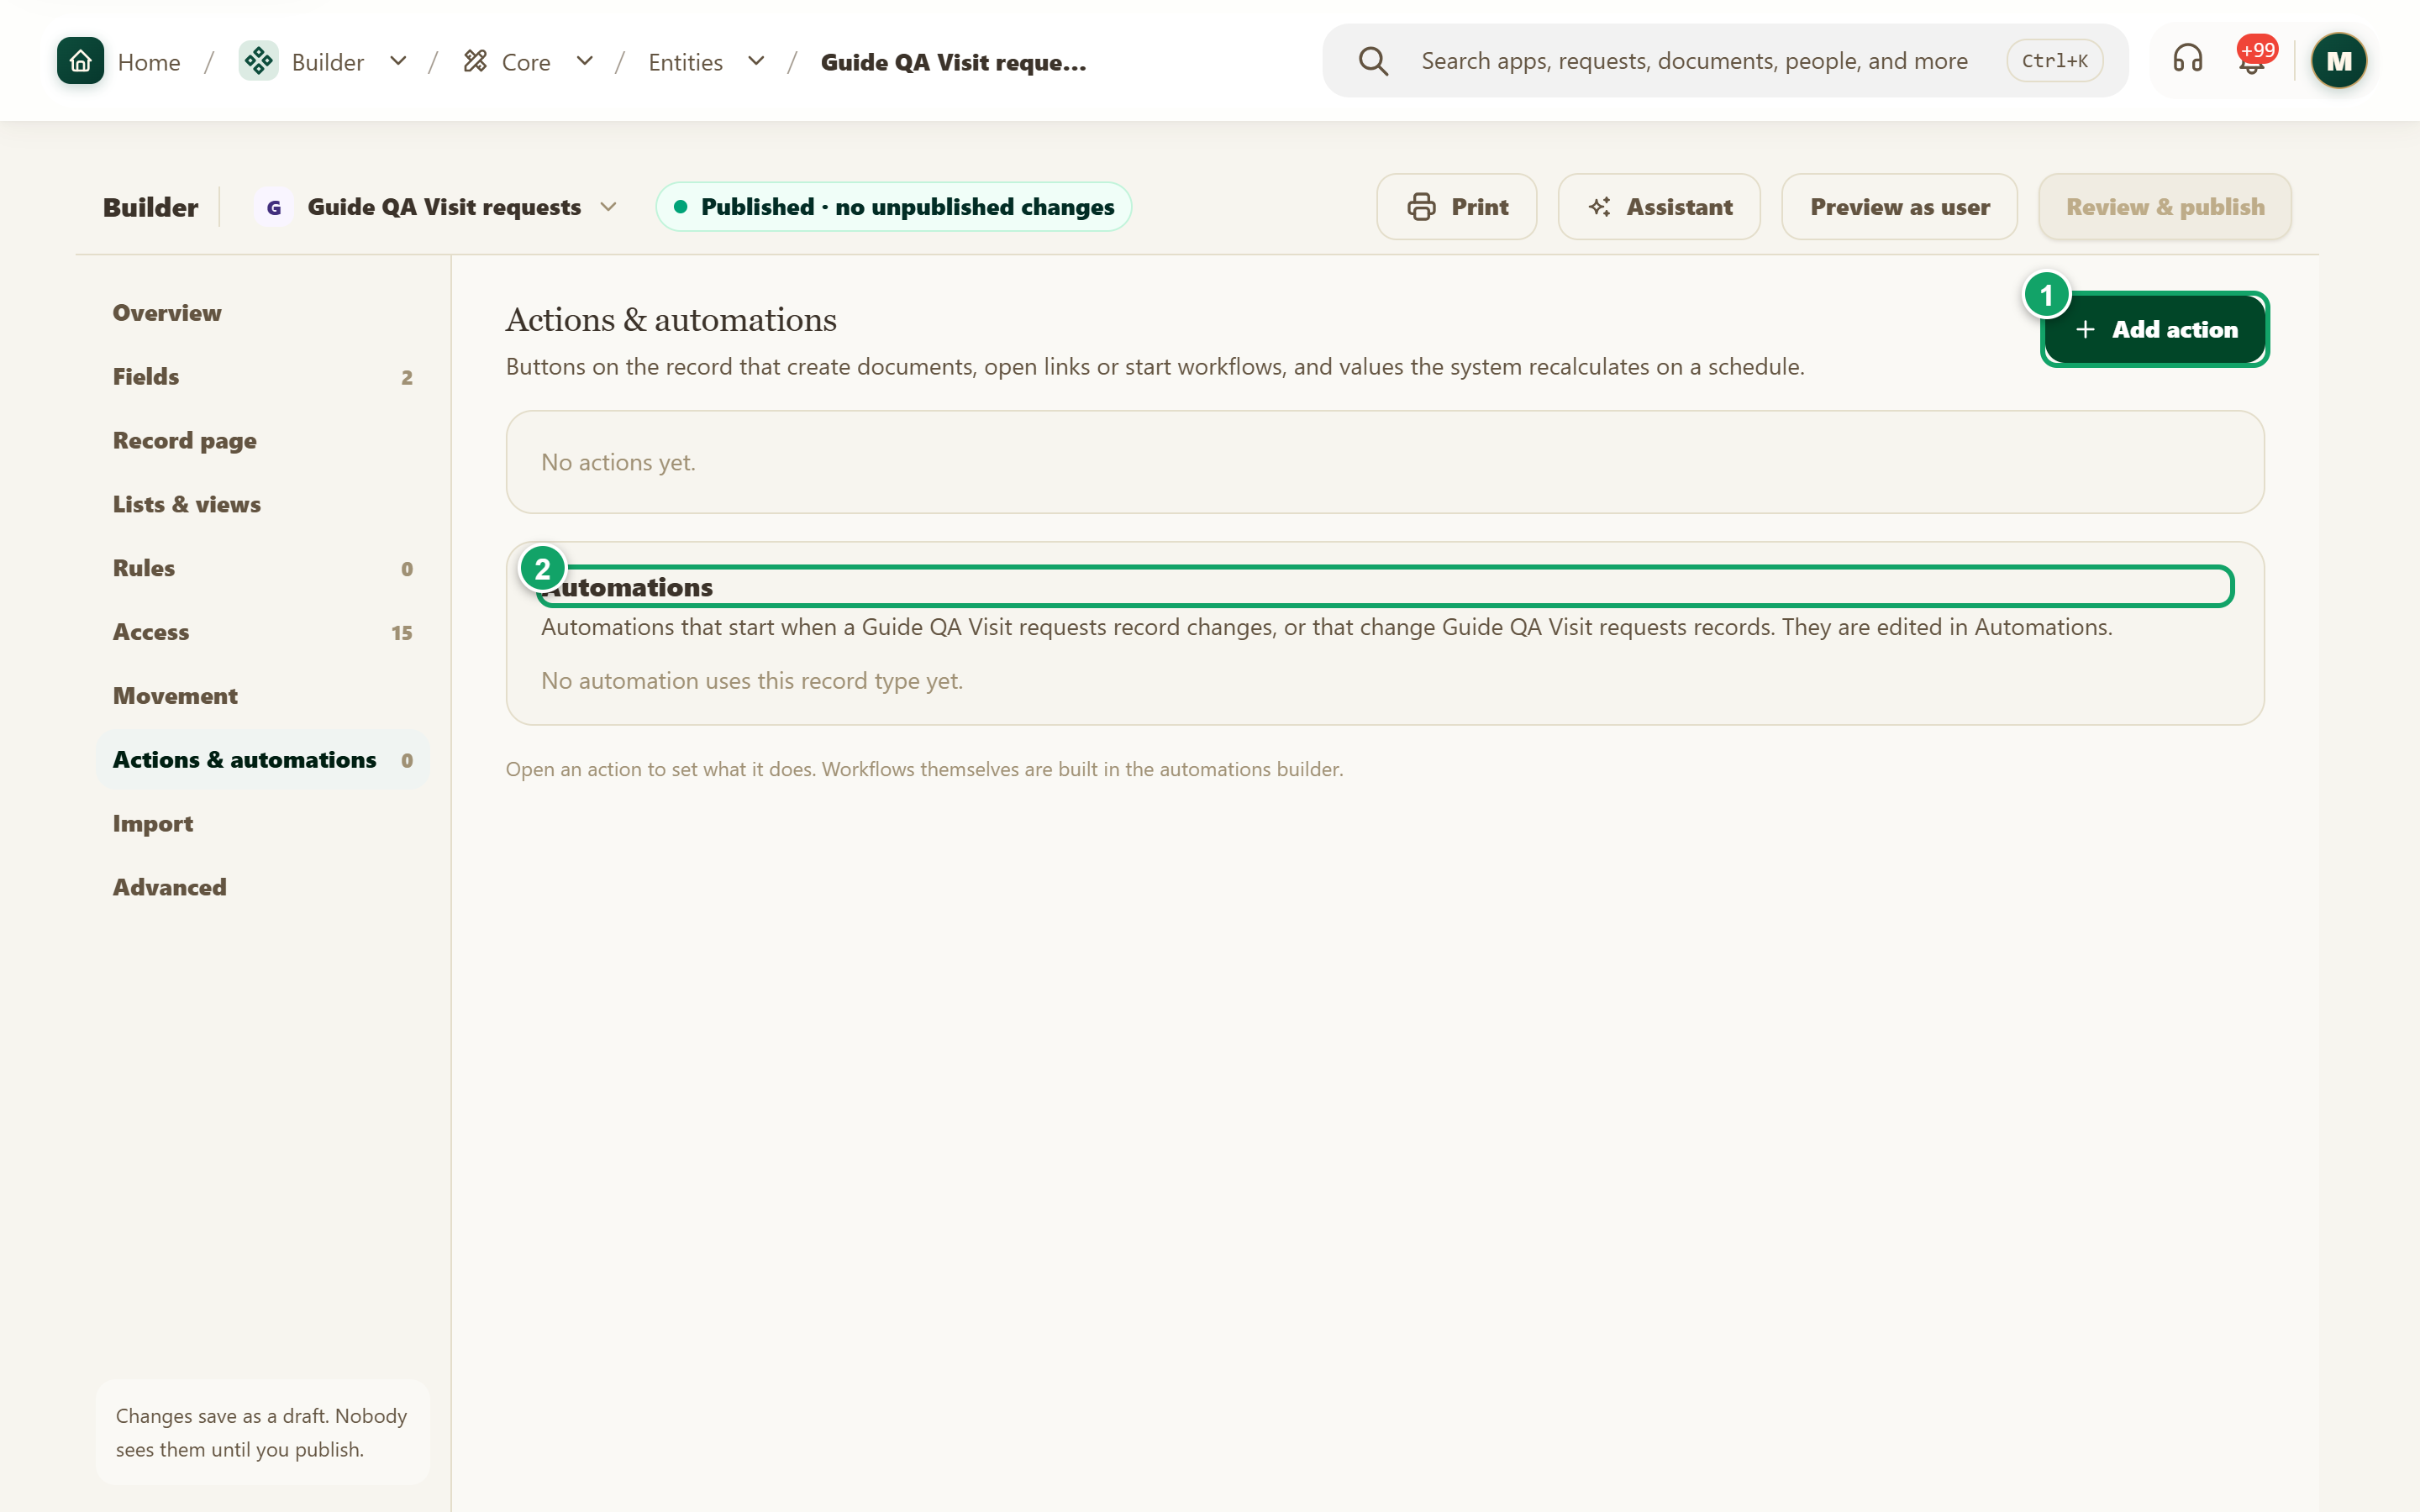
\includegraphics[width=0.95\linewidth,height=0.72\textheight,keepaspectratio]{figures/screens/ch06-ws-actions-en.png}
\caption{The “Actions \& automations” section}
\label{fig:builder-actions-screen}
\shotnote{The section shows the type’s buttons and its linked automations, both empty on the test type. ① “Add action”: creates a new button and opens it so you set what it does. ② “Automations”: a view-only list of automations started by, or changing, this type’s records.}
\end{figure}


\begin{table}[H]
\centering
\caption{What do you find here?}
\label{tab:builder-actions-data}
\begin{tabularx}{\linewidth}{R{3.6cm} Y}
\rcHeaderRow
\thh{Part} & \thh{Content and action}\\
Actions & Each action shows its kind, “Word document”, “Spreadsheet”, “Link” or “Workflow”, and who can run it: it “Needs” a given verb, or “Anyone who can change the record”.\\
Add action & Creates a “New action” in the draft and opens it in “Fields”, where you choose what it does and the template or workflow it uses.\\
Automations & A view-only list of automations that “Starts on a change” of a record of this type or that “Changes records”, with their state: “Live”, “Not published” or “Paused”. They are edited on the automations page.\\
Recalculated on a schedule & Calculated fields the system recalculates “Daily”, “Weekly” or “Monthly”; shown only when they exist.\\
\end{tabularx}
\end{table}

\begin{figure}[H]
\centering
\begin{tikzpicture}[node distance=0.5cm]
\node[entity] (action) {Action button on the record};
\node[entityOpt,below right=0.7cm and 0.3cm of action] (tpl) {Document template};
\node[entityOpt,below left=0.7cm and 0.3cm of action] (sop) {Workflow};
\draw[dependsOnOpt] (action.south) -- ++(0,-0.3) -| (tpl.north);
\draw[dependsOnOpt] (action.south) -- ++(0,-0.3) -| (sop.north);
\end{tikzpicture}
\rclegend
\caption{What an action calls}
\label{fig:builder-actions-model}
\shotnote{The figure shows that the button does not work on its own but calls something ready: a document template you prepare on the template pages, or a workflow you build in automations. So prepare the template or workflow first, then create the action and link it.}
\end{figure}

\subsection{Steps and check}
\begin{enumerate}
\item Prepare the template or workflow the button will call.
\item Open the record type, choose “Actions \& automations”, then press “Add action”.
\item In the field that opens, name the action, choose its kind and the template or workflow, then set the verb needed to run it.
\item Publish the changes, then open a test record and press the button.
\end{enumerate}

\textbf{Check and recovery:} the button should appear on the record for those holding the required verb, and it should produce the document or start the workflow. If the action shows the kind “Not set up”, open it and finish choosing what it does; if the button does not appear for a user, review the verb it needs.

\clearpage
\section{Movement}
\label{sec:builder-feature-movement}

Movement is a specialist setting for records that move an amount or quantity from one record to another, such as transfers between budget lines or between stores. Each record names where the amount comes from and where it goes; KayanOS keeps both sides equal and posts them together when the record reaches a status you choose. Most record types do not need this section.

\textbf{Path and who uses it:} record type → “Movement”. Used by whoever builds financial or stock record types.

\begin{rcnote}[Example: Horizon]
“Visit requests” does not need movement. But if Horizon created a type for transfers between branch budget lines, each approved transfer would post the amount from the Aleppo line to the Damascus line in one step. The system administrator does not go past the conditions in ②, because the requests type does not need them.
\end{rcnote}

\begin{figure}[H]
\centering
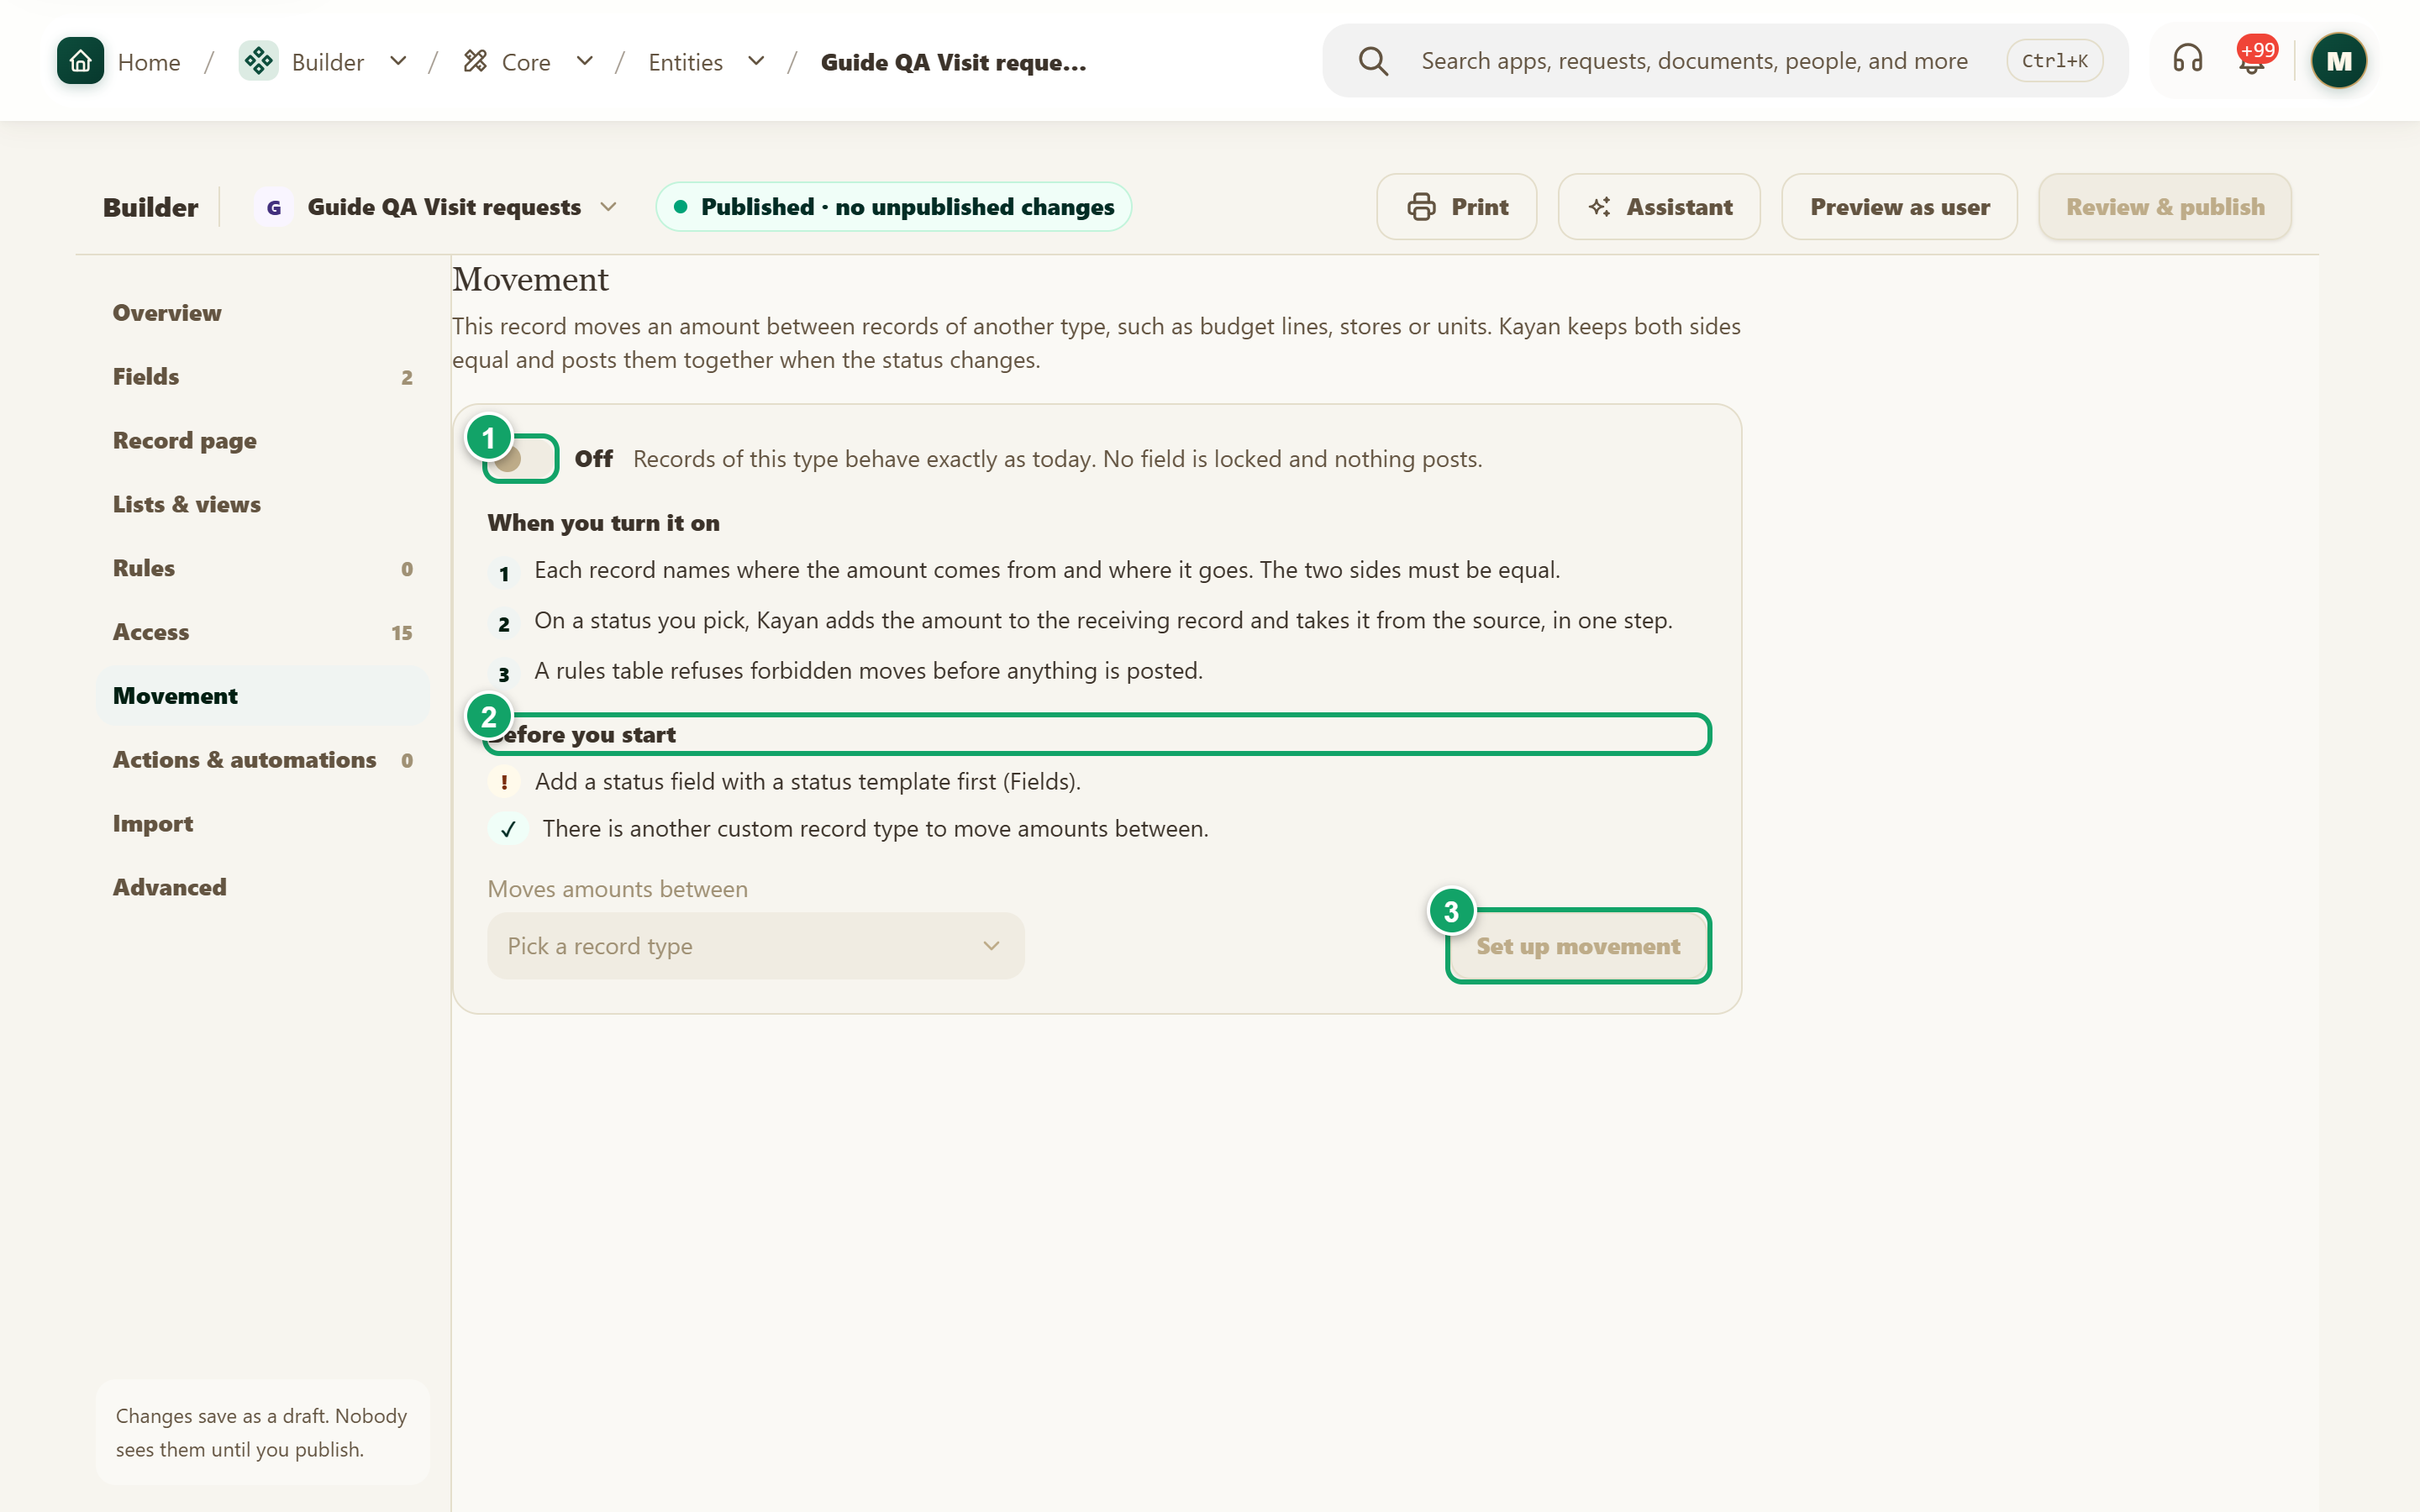
\includegraphics[width=0.95\linewidth,height=0.72\textheight,keepaspectratio]{figures/screens/ch06-ws-movement-en.png}
\caption{The “Movement” section while off}
\label{fig:builder-movement-screen}
\shotnote{The section explains what movement does once on and checks its conditions before you start. The warning mark shows because the test type has no status field. ① The switch: off, so nothing posts. ② “Before you start”: the conditions to meet, with a mark for each. ③ “Set up movement”: starts the setup after you choose the type amounts move between.}
\end{figure}


\begin{table}[H]
\centering
\caption{What do you need and set?}
\label{tab:builder-movement-data}
\begin{tabularx}{\linewidth}{R{3.6cm} Y}
\rcHeaderRow
\thh{Part} & \thh{Meaning}\\
Before you start & A “Status” field with a status template on this type, and another custom record type amounts move between, with number fields for “in” and “out”. Movement does not work on built-in types.\\
Sides & Where the amount comes from and where it goes; the two must be equal.\\
Posting & The status at which the amount posts, and its effect: hold, post, release or reverse.\\
Rules & Refuses forbidden moves before anything is posted.\\
Period totals and Try it & Show totals for each period and test the setup before publishing.\\
\end{tabularx}
\end{table}

\begin{figure}[H]
\centering
\begin{tikzpicture}[node distance=0.5cm]
\node[stepBox] (a) {Movement record: draft};
\node[stepBox,below=of a] (b) {Reaches the posting status};
\node[stepBox,below=of b] (c) {Taken from source, added to receiver};
\draw[flowsTo] (a) -- (b);
\draw[flowsTo] (b) -- (c);
\end{tikzpicture}
\rclegend
\caption{When does the amount move?}
\label{fig:builder-movement-flow}
\shotnote{The diagram shows that the amount does not move when the record is created but when it reaches the status you chose for posting. At that point it is taken from the source and added to the receiver together, so one side never moves without the other.}
\end{figure}

\subsection{Steps and check}
\begin{enumerate}
\item Make sure the “Status” field and the receiving record type with in and out fields exist.
\item Open “Movement”, choose the type in “Moves amounts between”, then press “Set up movement”.
\item Set the “Sides”, “Posting” and “Rules” tabs, then use “Try it” before publishing.
\end{enumerate}

\textbf{Check and recovery:} after publishing, move a test record to the posting status and confirm both balances changed by the same amount. If you turn movement off later, amounts already posted stay as they are and only new records stop posting.

\clearpage
\section{Import}
\label{sec:builder-feature-import}

The “Import” section decides how people load and update this type's records from Excel and CSV files. Its core is “Import keys”: a field or set of fields, such as a code or number, that KayanOS uses to match each row in the file to an existing record, so it updates that record instead of creating a duplicate. When the option is off, import works as before and guesses matches by ID, code or name.

\textbf{Path and who uses it:} record type → “Import”. Used by whoever builds the record type, before the team starts updating records from files.

\begin{rcnote}[Example: Horizon]
The system administrator adds an import key based on the request number \en{HZN-VR-0001}, so Omar Haddad uploads an Excel file with updated visit dates and KayanOS updates the same requests without creating new ones. They add the key from ② and check it with ③.
\end{rcnote}

\begin{figure}[H]
\centering
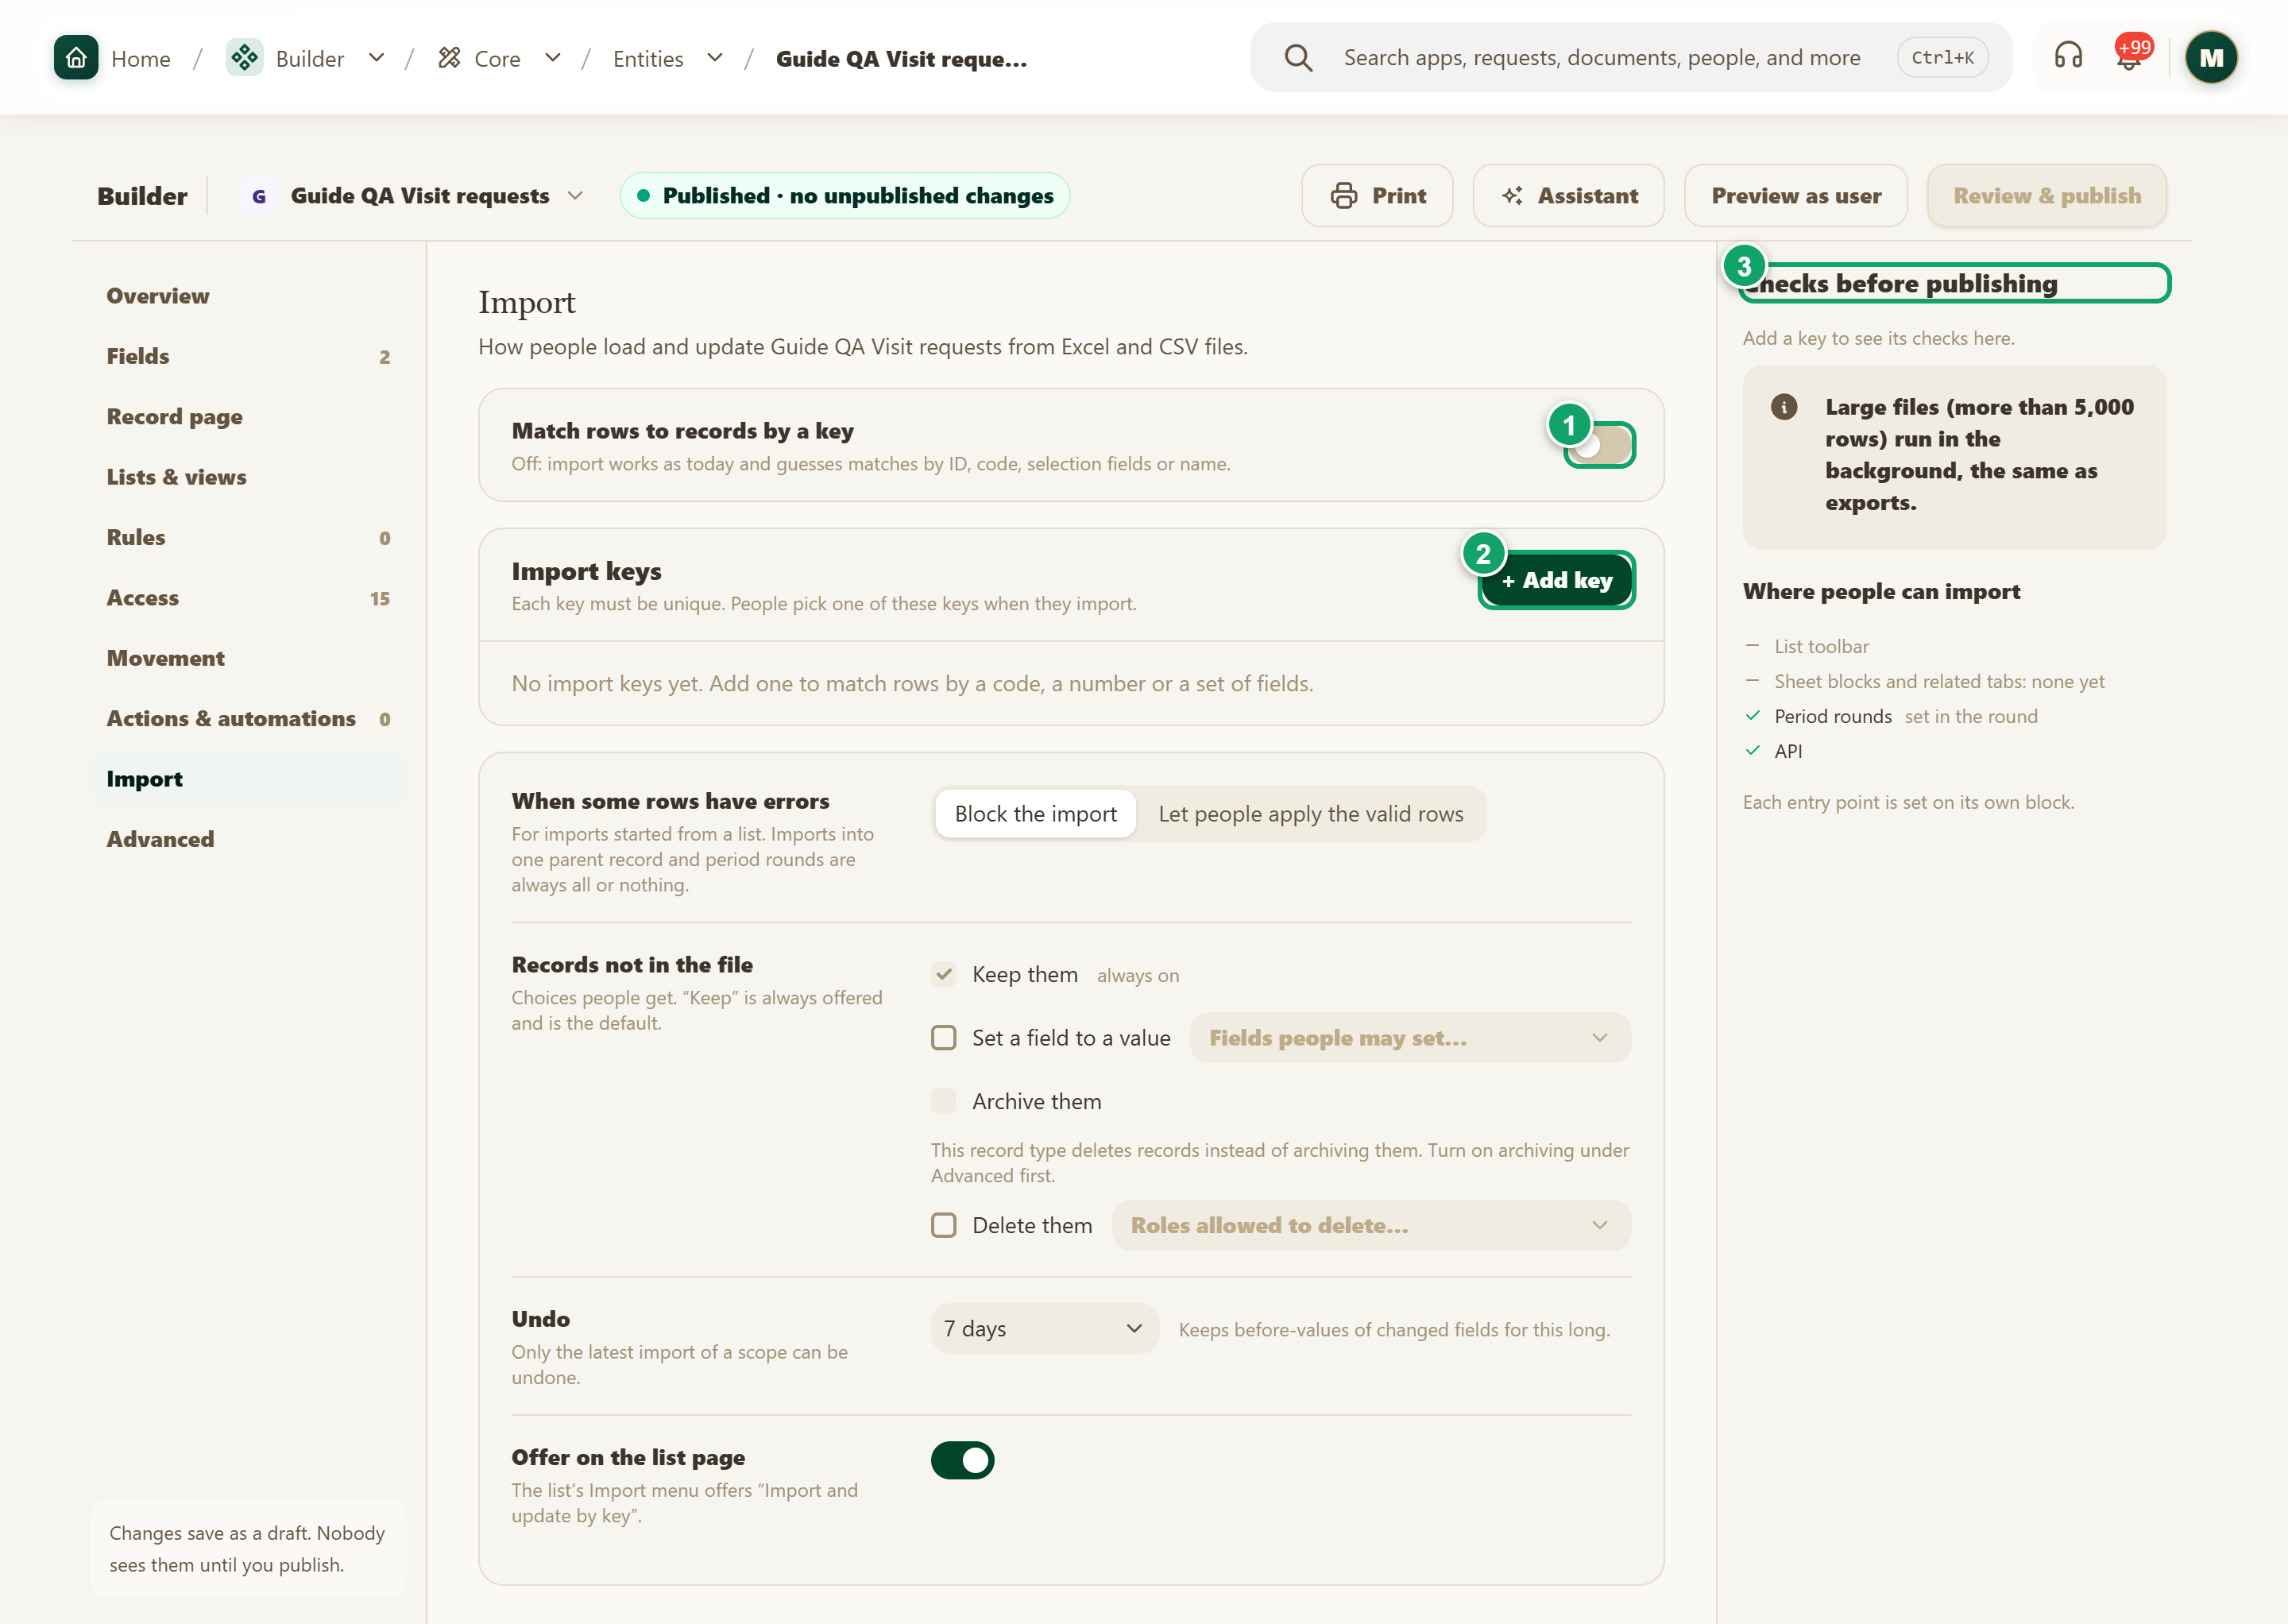
\includegraphics[width=0.95\linewidth,height=0.72\textheight,keepaspectratio]{figures/screens/ch06-ws-import-en.png}
\caption{The “Import” section}
\label{fig:builder-import-screen}
\shotnote{The section decides how records are updated from Excel and CSV files; matching by key is off here. ① The “Match rows to records by a key” switch. ② “+ Add key”: adds the field rows are matched by. ③ “Checks before publishing”: after you add a key, “Run check” shows here whether it is unique among saved records.}
\end{figure}


\begin{table}[H]
\centering
\caption{What do you find here?}
\label{tab:builder-import-data}
\begin{tabularx}{\linewidth}{R{3.6cm} Y}
\rcHeaderRow
\thh{Part} & \thh{Content and action}\\
Match rows to records by a key & Turns on import by key. When off, import guesses matches as before.\\
Import keys & Each key shows the fields it is “Made of”, where it is “Unique within”, its “Normalising”, such as ignoring spaces or leading zeros, whether it is “Backed by” a unique value, and its status, “Ready” or “Problem”.\\
Behaviour & What happens “When some rows have errors”, block the import or allow the valid rows, what happens to records missing from the file, keep, archive or delete them, and how long the last import can be undone.\\
Checks before publishing & “Run check” confirms the key is unique among saved records and shows duplicate or empty ones.\\
\end{tabularx}
\end{table}

\begin{figure}[H]
\centering
\begin{tikzpicture}[node distance=0.5cm]
\node[stepBox] (a) {Add an import key};
\node[stepBox,below=of a] (b) {Run the check};
\node[stepBox,below=of b] (c) {Set the behaviour};
\node[stepBox,below=of c] (d) {Publish, then import a file};
\draw[flowsTo] (a) -- (b);
\draw[flowsTo] (b) -- (c);
\draw[flowsTo] (c) -- (d);
\end{tikzpicture}
\rclegend
\caption{Preparing import by key}
\label{fig:builder-import-flow}
\shotnote{The diagram puts the check right after adding the key, because a key whose value repeats across two records cannot tell which one to update. Then you decide what happens to errors and to records missing from the file, because a wrong choice here can archive or delete records. None of it works before you publish.}
\end{figure}

\subsection{Steps and check}
\begin{enumerate}
\item Open the record type, choose “Import”, then turn on “Match rows to records by a key”.
\item Press “+ Add key” and choose the field that identifies each record, such as the code or serial number.
\item Press “Run check” and fix any duplicate or empty records it shows.
\item Choose the right behaviour for errors and missing records, then publish the changes.
\end{enumerate}

\textbf{Check and recovery:} the key's status should be “Ready” and the check should show it is unique. If it shows that some records would share the same key, fix their values first. Only choose to delete records missing from the file on purpose, and use undo if an import goes wrong.

\clearpage
\section{Advanced}
\label{sec:builder-feature-advanced}

“Advanced” holds settings that rarely change after the start, such as the record's name in lists, preventing duplicates, parent–child records and the app where the type appears. They are part of the draft like the other sections, so they do not reach the team before publishing.

\textbf{Path and who uses it:} record type → “Advanced”. Used by whoever builds the type, usually at creation and then only when needed.

\begin{rcnote}[Example: Horizon]
The system administrator makes the visit request's “Record name” the serial number with the branch name, places the type in the “Branch services” app, and chooses “Archive records instead of deleting them” so no request is lost. Their choices match numbers ① and ④.
\end{rcnote}

\begin{figure}[H]
\centering
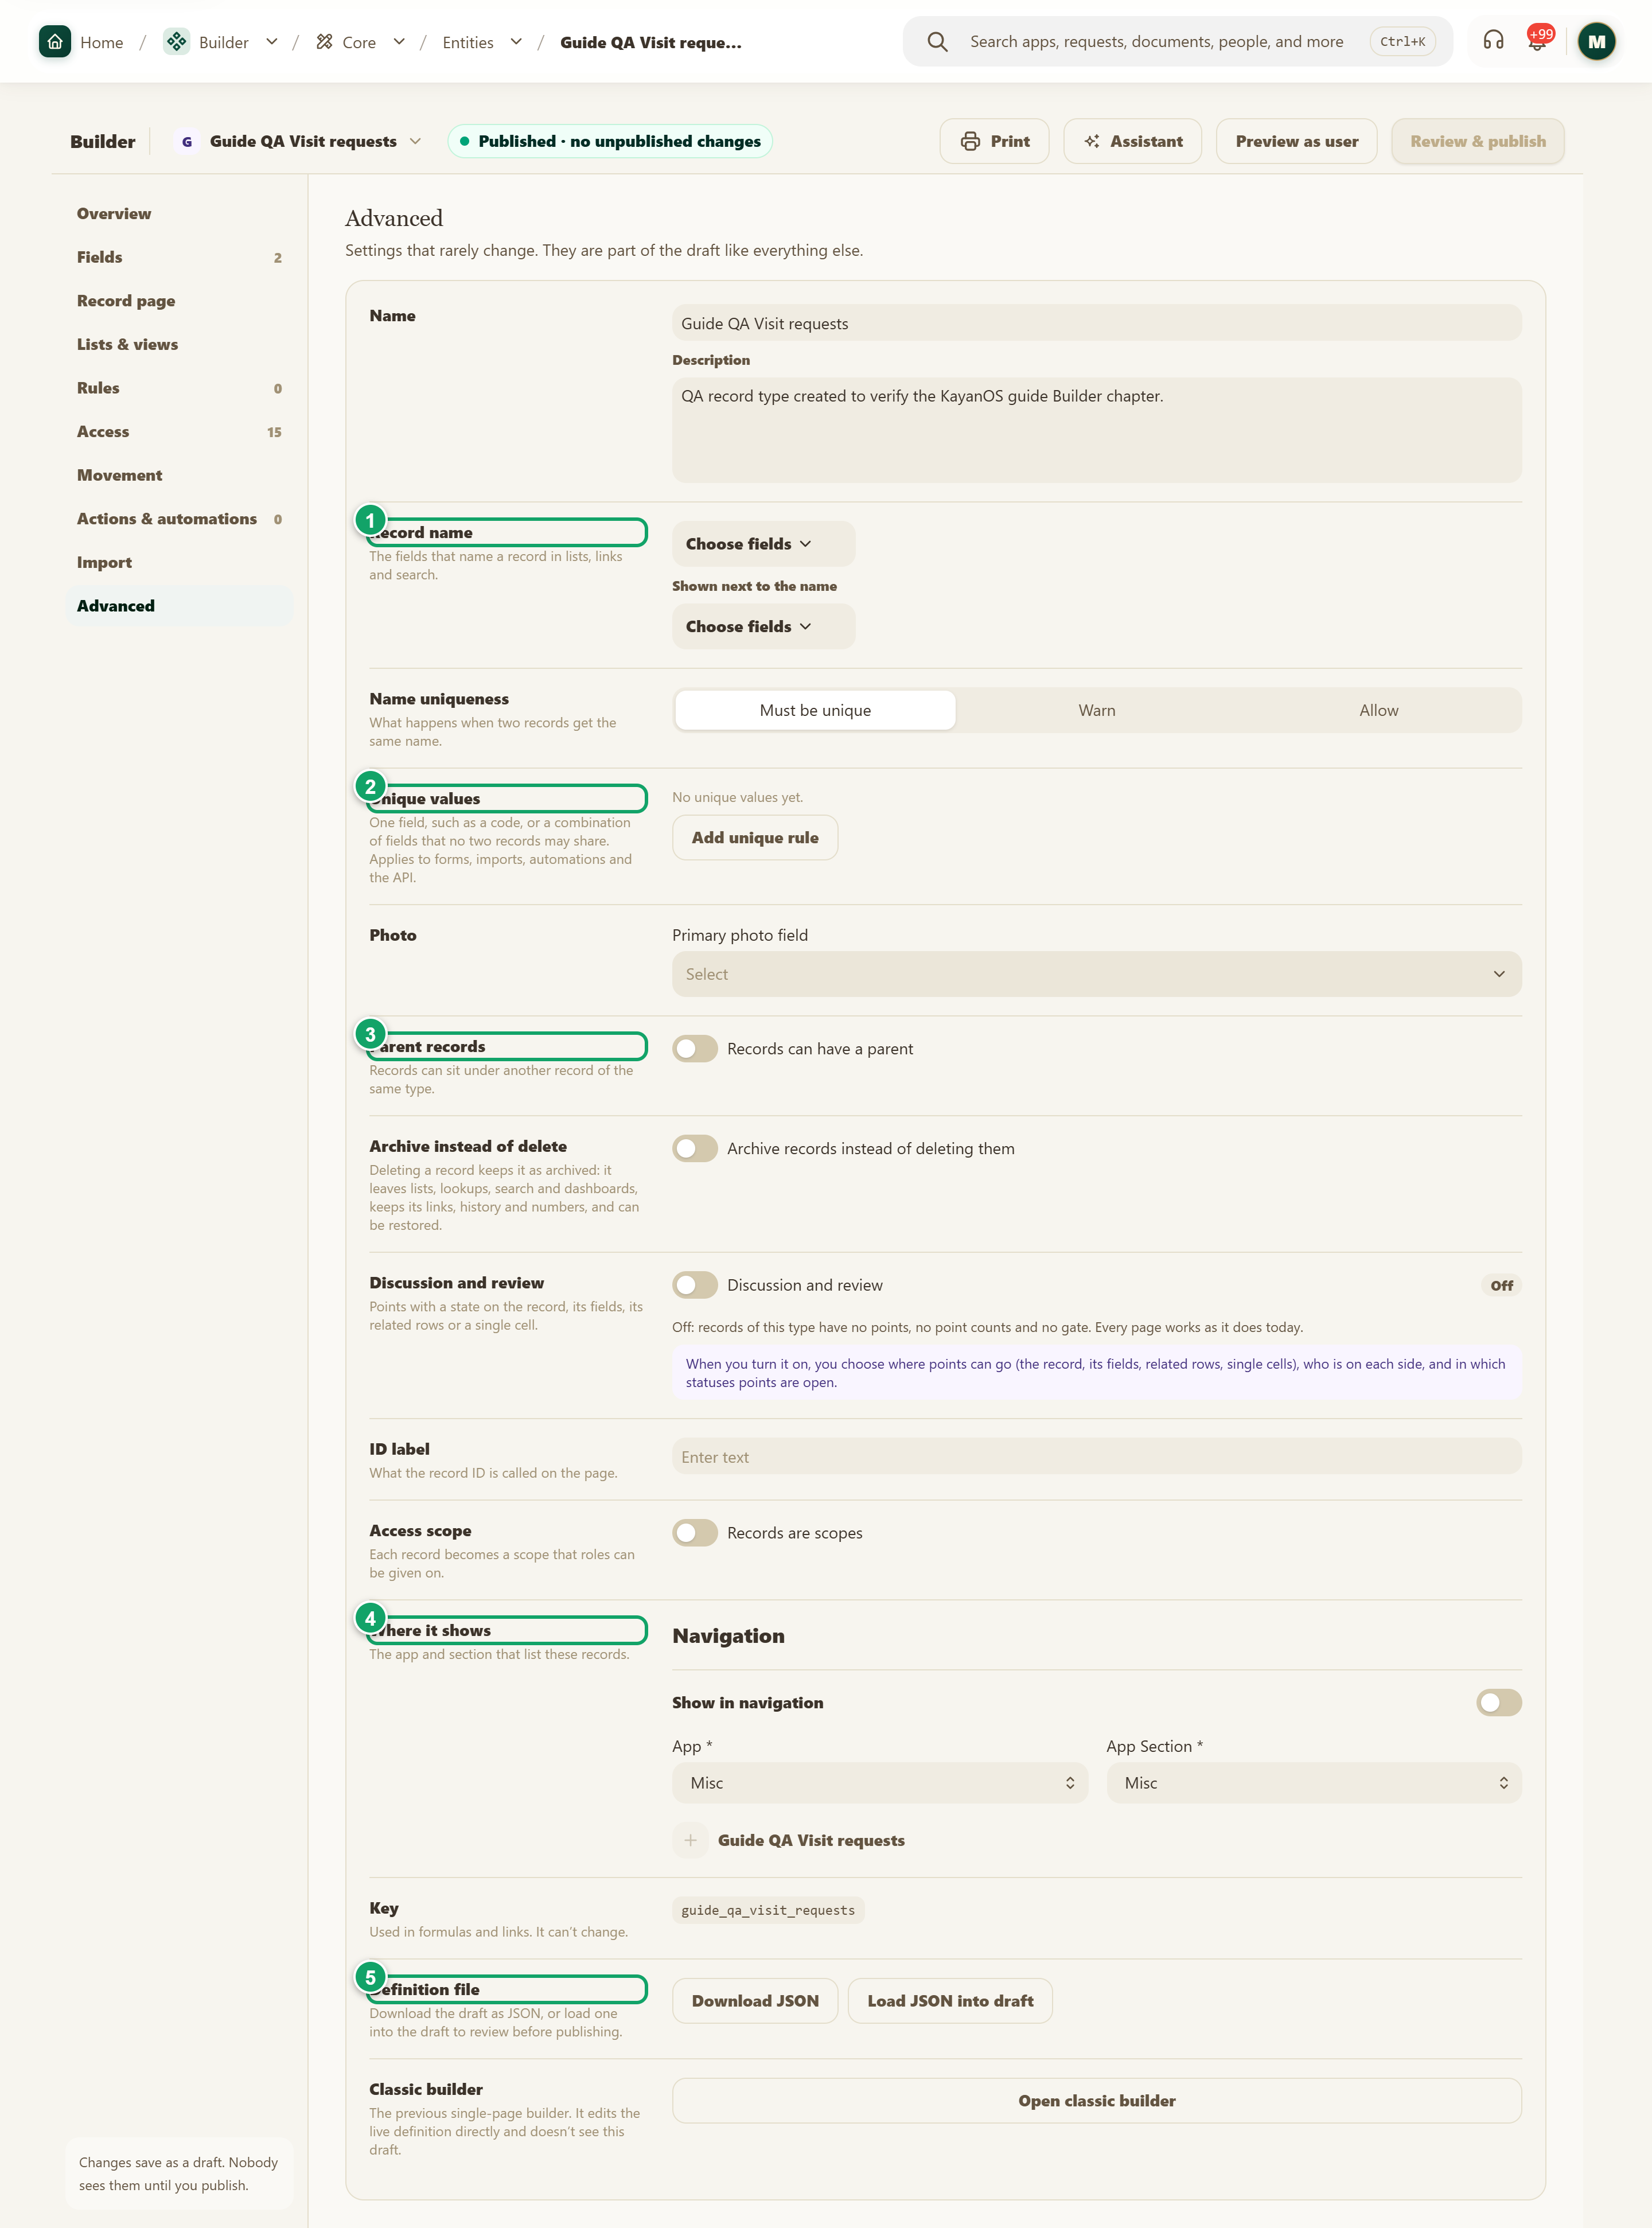
\includegraphics[width=0.95\linewidth,height=0.72\textheight,keepaspectratio]{figures/screens/ch06-ws-advanced-en.png}
\caption{The “Advanced” section}
\label{fig:builder-advanced-screen}
\shotnote{The section gathers rarely changed settings, shown here for the test record type. ① “Record name”: the fields that name a record. ② “Unique values”: prevents a repeated code or combination of values. ③ “Parent records”: allows parent–child records. ④ “Where it shows”: the app and section. ⑤ “Definition file”: download or load the setup as JSON.}
\end{figure}


\begin{table}[H]
\centering
\caption{What do you find here?}
\label{tab:builder-advanced-data}
\begin{tabularx}{\linewidth}{R{3.6cm} Y}
\rcHeaderRow
\thh{Setting} & \thh{Meaning}\\
Record name & The fields that name a record in lists, links and search, plus an optional field “Shown next to the name”.\\
Name uniqueness & What happens when two records get the same name: “Must be unique”, “Warn” or “Allow”.\\
Unique values & A field, such as a code, or a combination of fields that no two records may share, also in forms, imports and automations.\\
Photo & The field used as the record's main photo.\\
Parent records & Lets a record sit under another record of the same type, which makes the “Tree” view available.\\
Archive instead of delete & Moves a deleted record to the archive instead of removing it for good.\\
ID label & What the record ID is called on the page.\\
Access scope & Makes each record a scope roles can be given on, such as giving a branch manager rights on their branch only.\\
Where it shows & The “App” and “App Section” that list the records, “Show in navigation”, and the icon.\\
Key & Used in formulas and links; it can't change.\\
Definition file & “Download JSON” for a copy of the draft, or “Load JSON into draft” to review it before publishing.\\
Classic builder & The previous single-page builder; it edits the live definition directly and doesn't see the draft, so use it with care.\\
\end{tabularx}
\end{table}

\begin{figure}[H]
\centering
\begin{tikzpicture}[node distance=0.5cm]
\node[entity] (adv) {Advanced};
\node[entityOpt,below right=0.7cm and 0.3cm of adv] (tree) {Parent records};
\node[entityOpt,below left=0.7cm and 0.3cm of adv] (scope) {Access scope};
\node[entityOpt,below=0.7cm of tree] (treeview) {Tree view};
\node[entityOpt,below=0.7cm of scope] (roles) {Roles on one record};
\draw[dependsOnOpt] (adv.south) -- ++(0,-0.3) -| (tree.north);
\draw[dependsOnOpt] (adv.south) -- ++(0,-0.3) -| (scope.north);
\draw[dependsOnOpt] (tree) -- (treeview);
\draw[dependsOnOpt] (scope) -- (roles);
\end{tikzpicture}
\rclegend
\caption{Two settings that unlock other features}
\label{fig:builder-advanced-effects}
\shotnote{The figure shows that some advanced settings are a condition for features in other sections: turning on “Parent records” makes the “Tree” view available in lists, and turning on “Access scope” allows roles on a single record. So if one of these features is missing, start by reviewing this section.}
\end{figure}

\subsection{Steps and check}
\begin{enumerate}
\item Open the record type and choose “Advanced”.
\item Choose a “Record name” from fields that really identify the record, such as the serial number.
\item Use “Add unique rule” for fields that must not repeat, and review the warning if duplicates already exist.
\item Review “Where it shows” to confirm the app and section, then publish the changes.
\end{enumerate}

\textbf{Check and recovery:} after publishing, records should appear in lists and search under the name you chose, and a duplicate unique value should be refused. Before any large change, use “Download JSON” to keep a copy of the setup.

\clearpage
\section{Review \& publish}
\label{sec:builder-feature-publish}

The “Builder” workspace saves every change as a draft, and nobody else sees those changes until you publish them. “Review \& publish” shows all the changes before publishing and blocks it while a problem remains to be fixed. Each publish creates a new version you can return to later.

\textbf{Path and who uses it:} record type → “Review \& publish”. Used by whoever builds the type after finishing a set of changes.

\begin{rcnote}[Example: Horizon]
Before launching “Visit requests”, the system administrator uses “Preview as user” to see the page as Omar Haddad sees it, publishes the first version and asks Omar to try a request for the Aleppo Branch visit. They use ③ before publishing from ④.
\end{rcnote}

\begin{figure}[H]
\centering
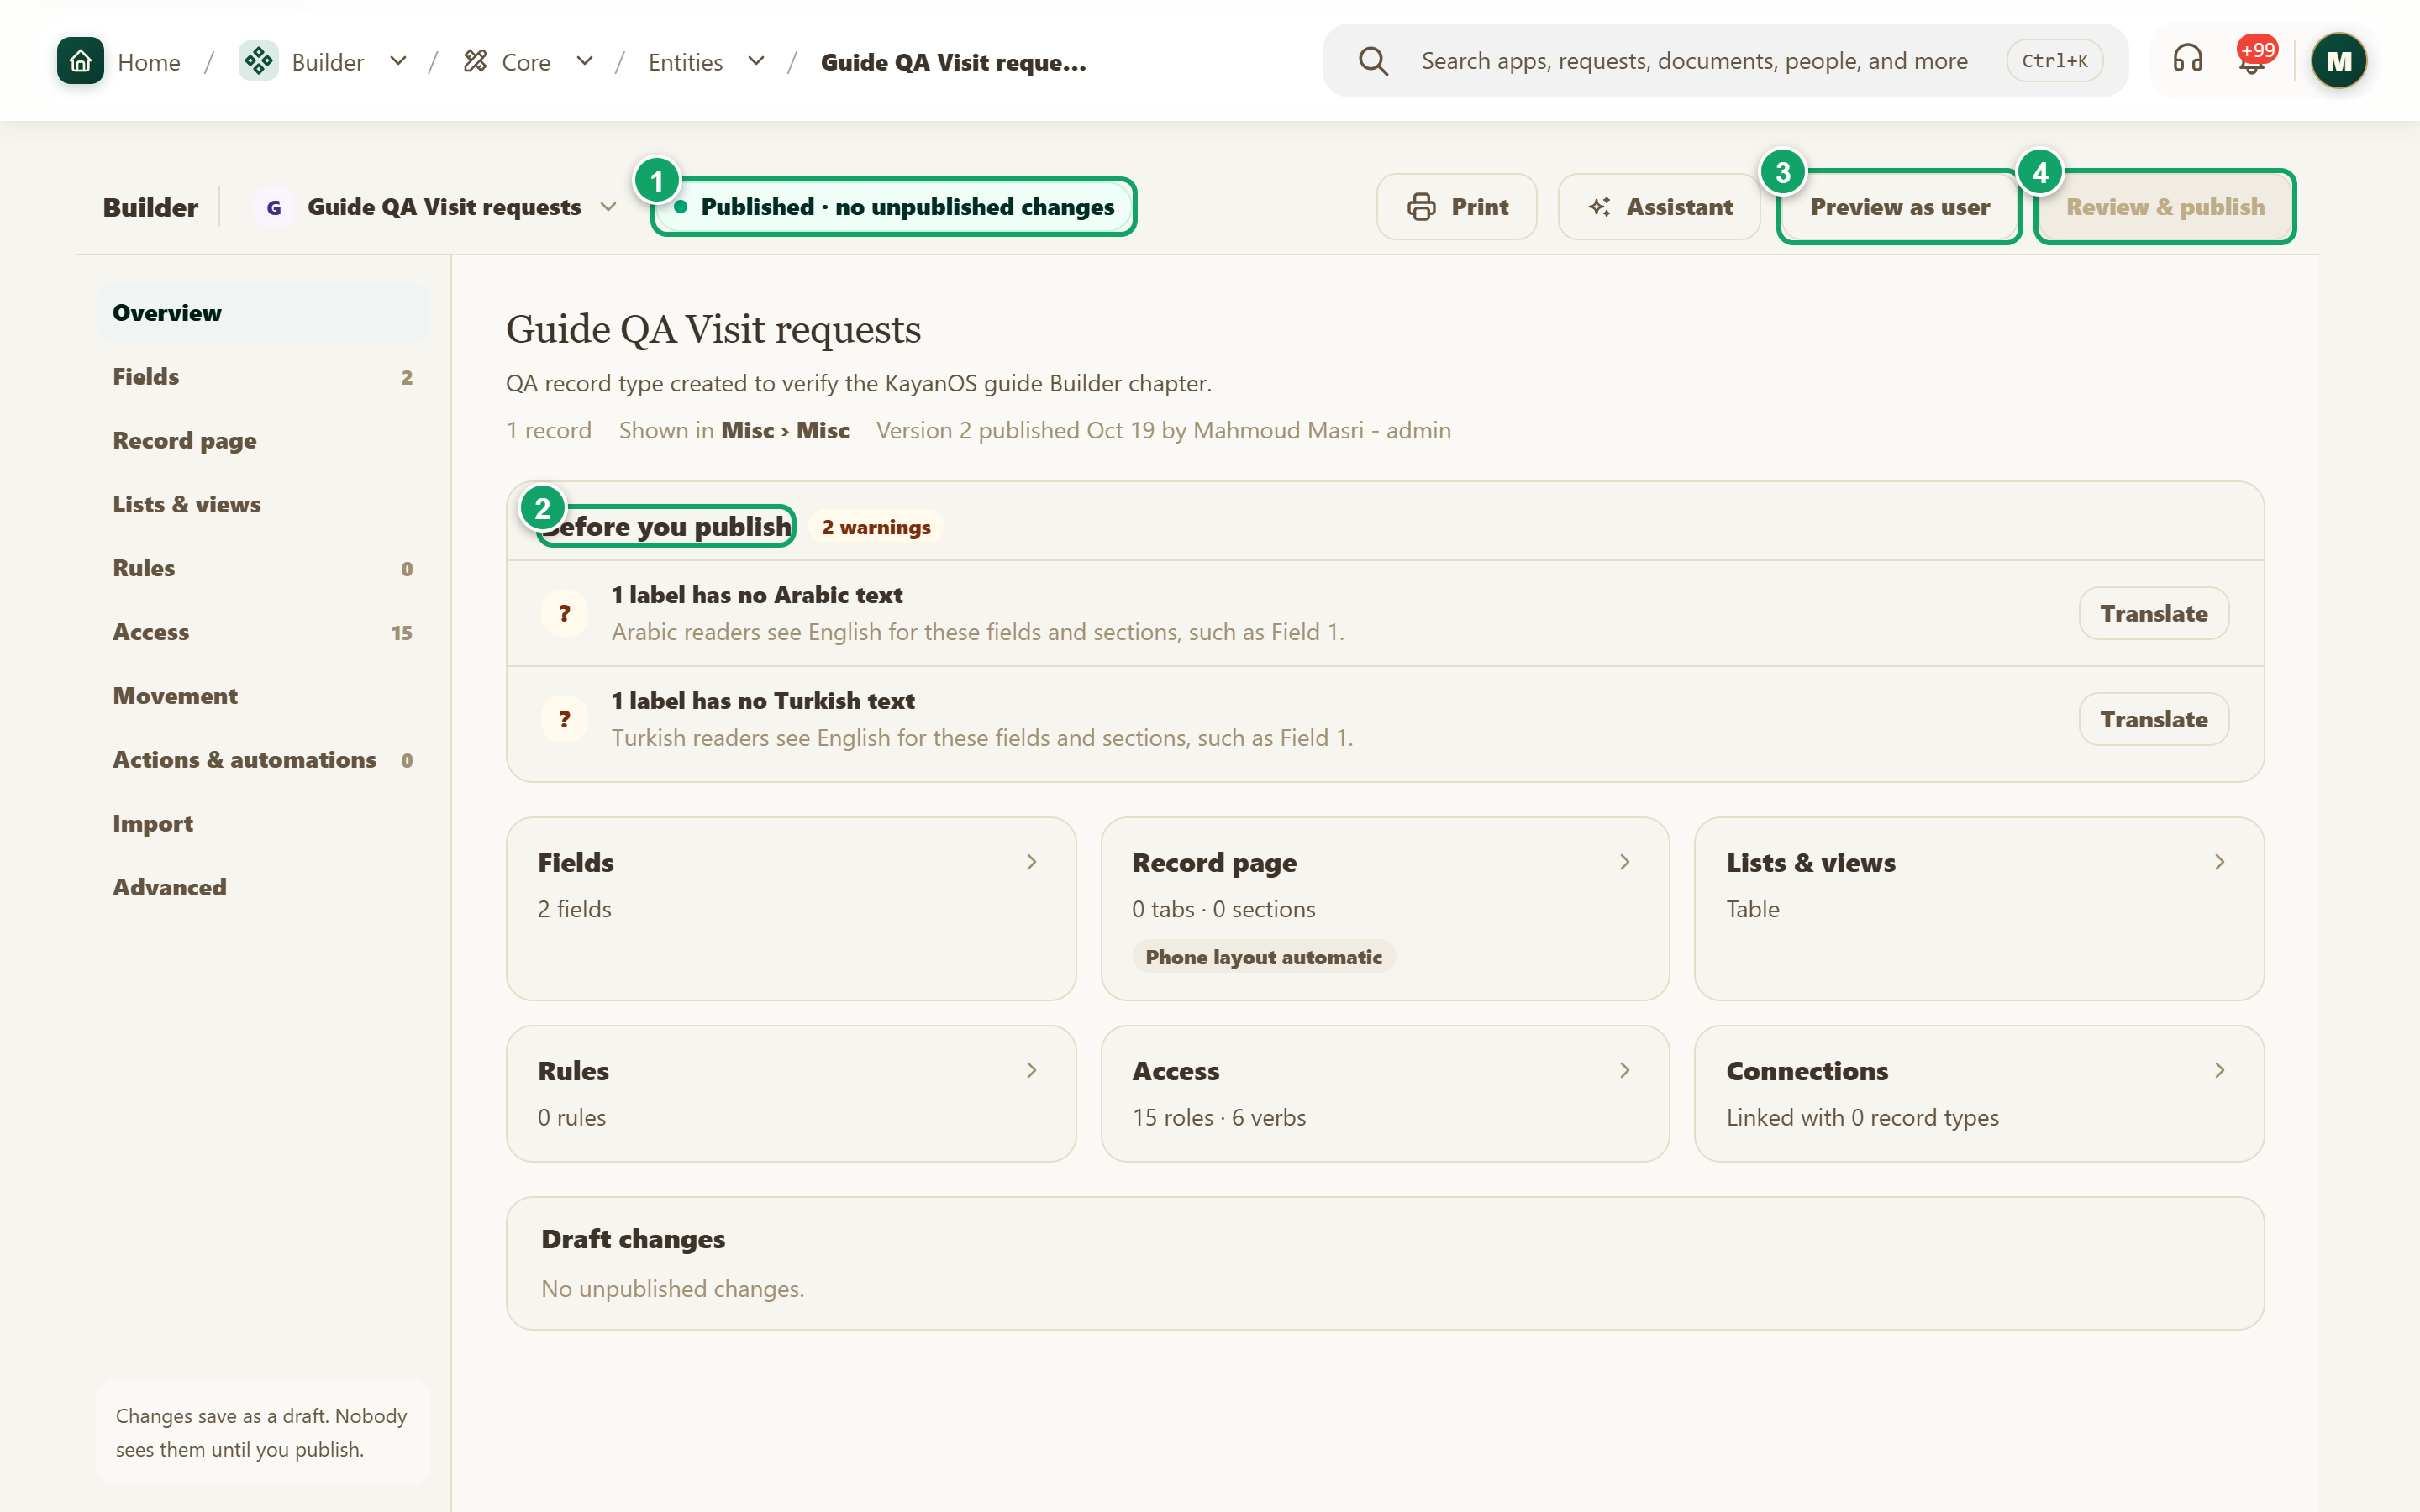
\includegraphics[width=0.95\linewidth,height=0.72\textheight,keepaspectratio]{figures/screens/ch06-ws-overview-en.png}
\caption{“Overview” after publishing}
\label{fig:builder-publish-screen}
\shotnote{“Overview” summarizes the type’s state and what to fix before publishing. The test type here is published as version 2 after testing this chapter, with translation warnings that do not block publishing. ① The state: “Published · no unpublished changes”. ② “Before you publish”: problems and warnings. ③ “Preview as user”: try the type as users see it. ④ “Review \& publish”: opens the change list and the publish button.}
\end{figure}


\begin{table}[H]
\centering
\caption{What do you find here?}
\label{tab:builder-publish-data}
\begin{tabularx}{\linewidth}{R{3.6cm} Y}
\rcHeaderRow
\thh{Item} & \thh{Meaning and action}\\
Draft & The type has unpublished changes. “Published · no unpublished changes” means the team sees the latest version you built.\\
Overview & A summary of fields, page, lists and rules; “Before you publish” lists the problems that block publishing and the warnings.\\
Preview as user & Shows the type as the user will see it, before publishing.\\
Review \& publish & Opens “Review changes” for every change, then publishes them together with the publish button.\\
Version history & Lists earlier versions and lets you “Restore” one of them.\\
Discard draft & Deletes the unpublished changes and returns the type to the last published version.\\
\end{tabularx}
\end{table}

\begin{figure}[H]
\centering
\begin{tikzpicture}[node distance=0.5cm]
\node[stepBox] (a) {Changes saved as a draft};
\node[stepBox,below=of a] (b) {Fix “Before you publish”};
\node[stepBox,below=of b] (c) {Preview as user};
\node[stepBox,below=of c] (d) {Publish: a new version};
\draw[flowsTo] (a) -- (b);
\draw[flowsTo] (b) -- (c);
\draw[flowsTo] (c) -- (d);
\end{tikzpicture}
\rclegend
\caption{From draft to published version}
\label{fig:builder-publish-flow}
\shotnote{The diagram shows that publishing is a deliberate step taken by whoever builds the type, not an automatic result of saving. The draft collects changes safely, none of them reaches the team before the problems are fixed and you publish, and each publish becomes a version you can restore.}
\end{figure}

\subsection{Steps and check}
\begin{enumerate}
\item Open “Overview”, review “Before you publish” and fix every problem that blocks publishing.
\item Press “Preview as user” and review the page and lists as the team will see them.
\item Press “Review \& publish”, review the list of changes, then press the publish button.
\item Create a test record from the type's list, then reopen it and confirm its values were saved.
\end{enumerate}

\textbf{Check and recovery:} a message should say the type was “Published as version” with its number, and the status should change to “Published · no unpublished changes”. If a problem appears after publishing, open “Version history” and restore the previous version, then correct the draft and publish again.

\clearpage
\section{Apps \& Navigation}
\label{sec:builder-feature-navigation}

The “Apps \& Navigation” page decides what members see in the app list and in what order. From here you add an app or a section, drag modules to reorder them or move them between sections, change icons, and show or hide items. A module here is any navigation item: a record type, a form, a dashboard, a page or a built-in page.

\textbf{Path and who uses it:} “Builder” → “Core” → “Apps \& Navigation”. Available only to the organization owner and administrator.

\begin{rcnote}[Example: Horizon]
The system administrator adds a “Branch services” app with a “Visits” section, drags “Visit requests” into it and saves, so Omar Haddad finds it in the app list on his next page load. They add the app from ① and save from ③.
\end{rcnote}

\begin{figure}[H]
\centering
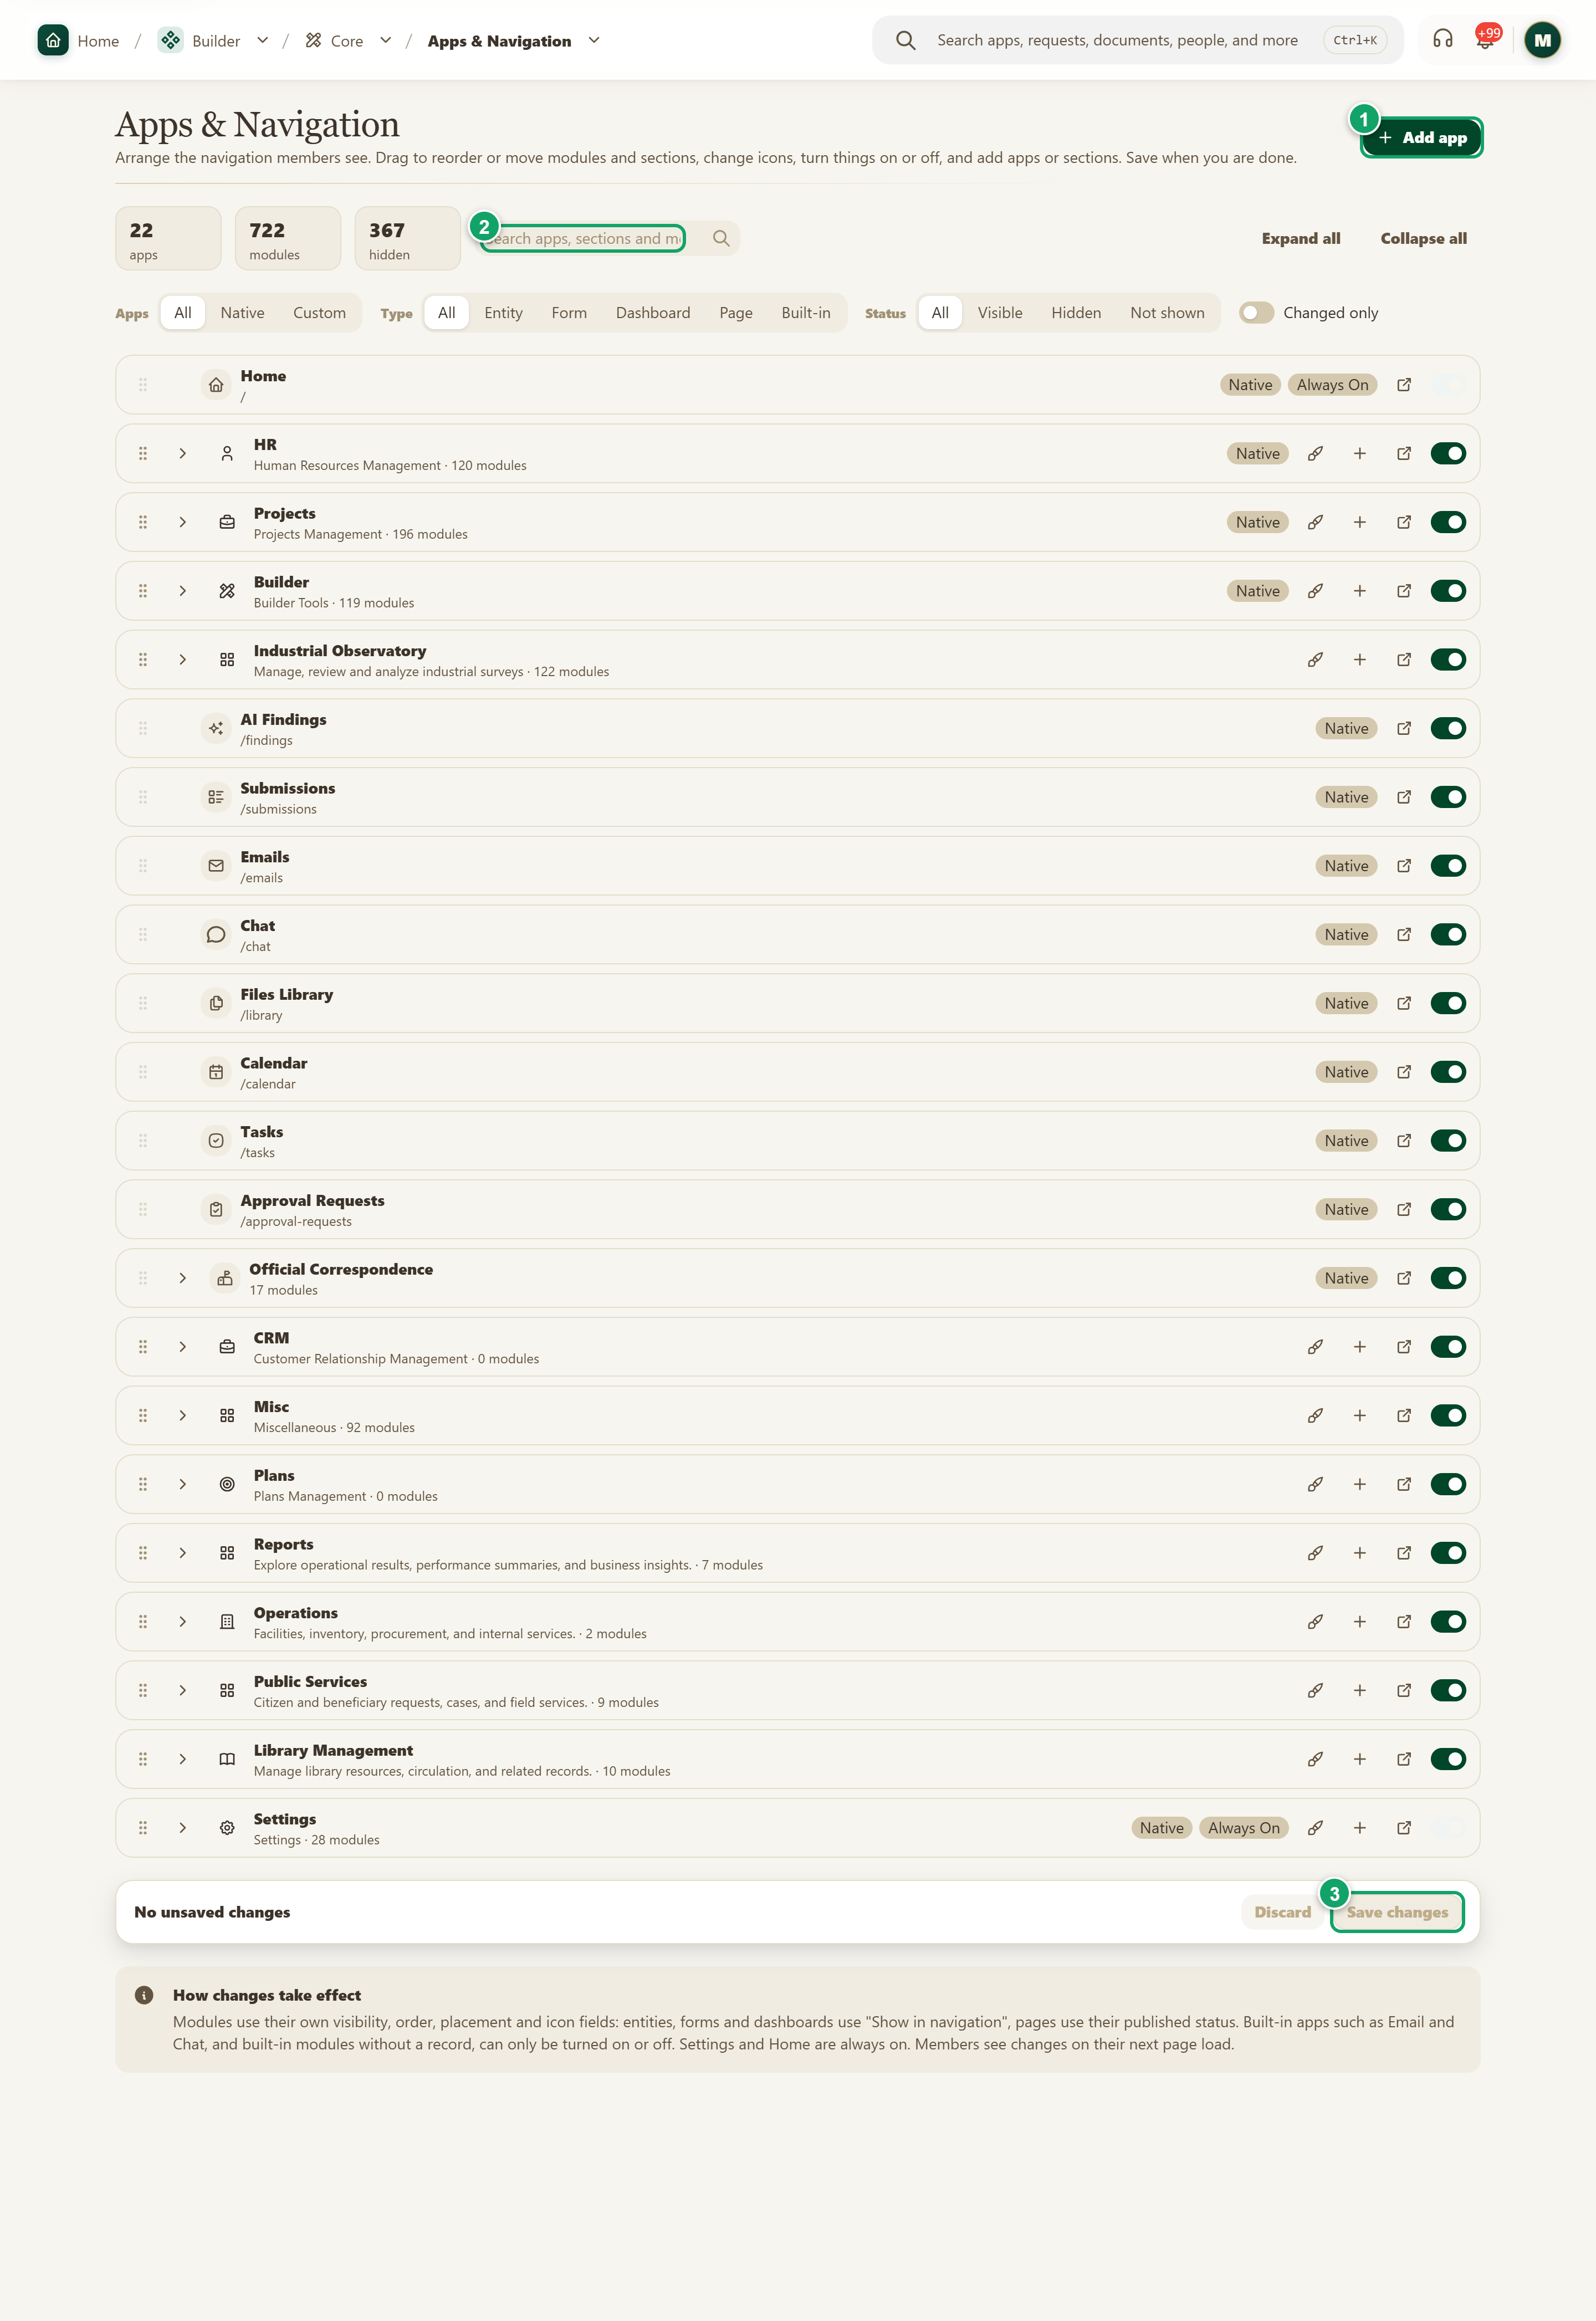
\includegraphics[width=0.95\linewidth,height=0.72\textheight,keepaspectratio]{figures/screens/ch06-navigation-en.png}
\caption{The “Apps \& Navigation” page}
\label{fig:builder-navigation-screen}
\shotnote{The page shows every app, section and module members see, with the state of each. The apps shown belong to the test organization. ① “Add app”: creates a new app. ② Search: finds an app, section or module quickly. ③ “Save changes”: saves order and switches; a new section does not need it.}
\end{figure}


\begin{table}[H]
\centering
\caption{What do you find here?}
\label{tab:builder-navigation-data}
\begin{tabularx}{\linewidth}{R{3.6cm} Y}
\rcHeaderRow
\thh{Part} & \thh{Content and action}\\
Add app and Add section & Creates a new app, or a section inside an app. The section is saved right away, without pressing save.\\
Dragging, icons and switches & Reorder apps, sections and modules by dragging, change the icon, and turn an item on or off. These changes need “Save changes”.\\
Filters & “Apps”: All, Native or Custom; “Type”: Entity, Form, Dashboard, Page or Built-in; “Status”: Visible, Hidden or Not shown; and “Changed only”.\\
Save changes and Discard & Saves the order and switches or undoes them. Members see the changes on their next page load.\\
Built-in items & Built-in apps such as Email and Chat can only be turned on or off, while Settings and Home are always on.\\
\end{tabularx}
\end{table}

\begin{figure}[H]
\centering
\begin{tikzpicture}[node distance=0.5cm]
\node[entity] (app) {App};
\node[entity,below=0.7cm of app] (section) {Section};
\node[entityOpt,below right=0.7cm and 0.3cm of section] (type) {Record type or form};
\node[entityOpt,below left=0.7cm and 0.3cm of section] (dash) {Dashboard or page};
\draw[dependsOn] (app) -- (section);
\draw[dependsOnOpt] (section.south) -- ++(0,-0.3) -| (type.north);
\draw[dependsOnOpt] (section.south) -- ++(0,-0.3) -| (dash.north);
\end{tikzpicture}
\rclegend
\caption{How navigation is built}
\label{fig:builder-navigation-tree}
\shotnote{The figure shows that an app holds sections, and a section holds the modules members open, such as record types, forms and dashboards. So create the app and section first and then drag the module into it; a built-in app does not receive new modules.}
\end{figure}

\subsection{Steps and check}
\begin{enumerate}
\item Open “Apps \& Navigation” and press “Add app” if the work has no suitable app.
\item Add a section with the add button on the app's row, and give it a name and icon.
\item Find the record type or form, drag it into the section, and make sure it is “Visible”.
\item Press “Save changes”.
\end{enumerate}

\textbf{Check and recovery:} the message “Navigation saved.” should appear, and the app should show for members after they reload the page. If it does not show for a member, check that they can see the records, because a section with no item they are allowed to open is not shown. If the page refuses to move a module, move it to a section that is not built in.

\clearpage
\section{Work navigation}
\label{sec:builder-feature-work-navigation}

This page decides what each member sees first when the day starts: a «My desk» page for their role, a “Due for me” list that gathers the work waiting for them, a shared context such as the year or cycle that lists and dashboards follow, and saved views shown in menus with their counts. Every feature here is off until you turn it on.

\textbf{Path and who uses it:} “Builder” → “Core” → “Work navigation”. Available only to the organization owner and administrator.

\begin{rcnote}[Example: Horizon]
The system administrator turns on “Due for me” and adds to it the visit requests waiting for Sarah Al-Khatib's decision, so Sarah finds them in one place every morning instead of opening each list. They turn on the feature from ① and add the source from ②.
\end{rcnote}

\begin{figure}[H]
\centering
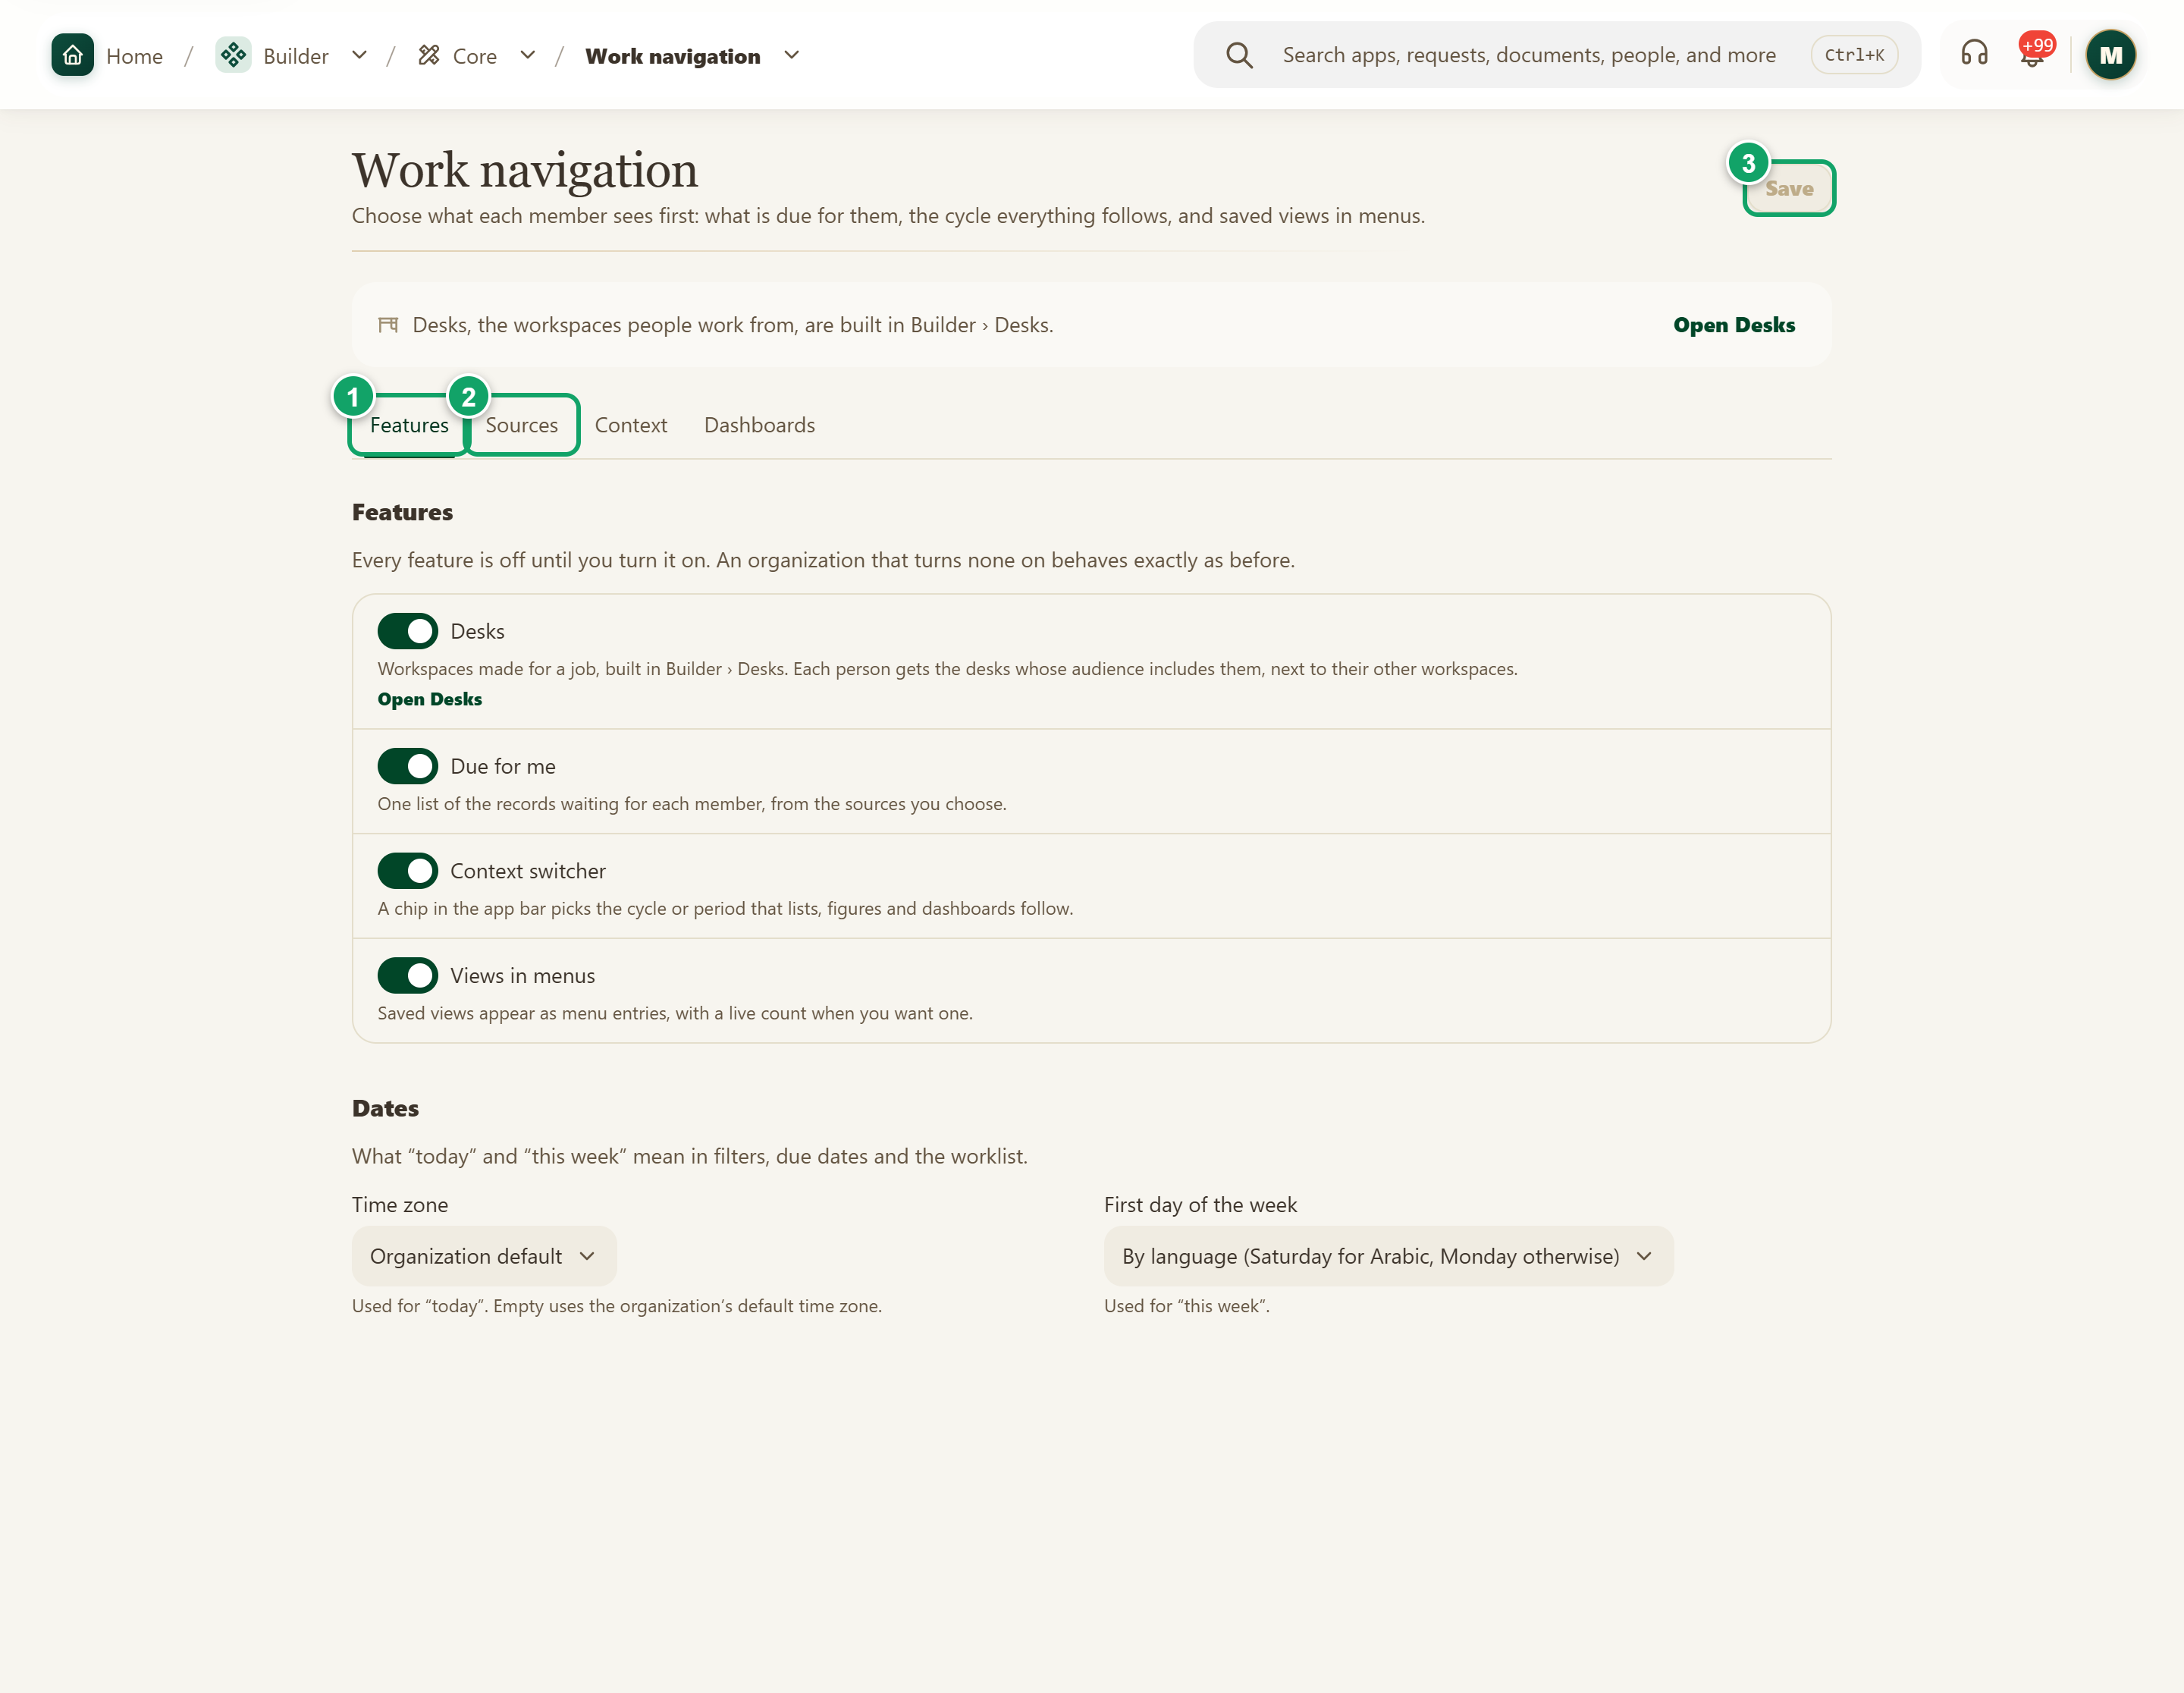
\includegraphics[width=0.95\linewidth,height=0.72\textheight,keepaspectratio]{figures/screens/ch06-work-navigation-en.png}
\caption{The “Work navigation” page}
\label{fig:builder-work-navigation-screen}
\shotnote{The page shows the start-page and due-work features, all off until you turn them on. ① “Features”: turns on «My desk», “Due for me” and more. ② “Sources”: what feeds the due list. ③ “Save”: saves the settings and stays disabled until you change something.}
\end{figure}


\begin{table}[H]
\centering
\caption{The page's tabs}
\label{tab:builder-work-navigation-data}
\begin{tabularx}{\linewidth}{R{3.6cm} Y}
\rcHeaderRow
\thh{Tab} & \thh{What do you set?}\\
Features & Turns on «My desk», “Due for me”, “Context switcher” and “Views in menus”, with the calendar, time zone and week start.\\
Sources & What feeds the “Due for me” list: transitions the member can run, records assigned to them, and built-in lists such as approvals.\\
Pages & «My desk» pages per role and for everyone else. They are start pages that never appear in menus, unlike the “Pages” page.\\
Context & A record type, such as the year or cycle, that chosen apps and sections follow; the member picks it from a chip in the app bar.\\
Dashboards & The default data scope for new dashboards, and a list of dashboards showing organization-wide data to switch to the viewer's permissions.\\
\end{tabularx}
\end{table}

\begin{figure}[H]
\centering
\begin{tikzpicture}[node distance=0.5cm]
\node[entity] (member) {Member};
\node[entityOpt,below right=0.7cm and 0.3cm of member] (desk) {My desk page};
\node[entityOpt,below left=0.7cm and 0.3cm of member] (due) {Due for me};
\draw[dependsOnOpt] (member.south) -- ++(0,-0.3) -| (desk.north);
\draw[dependsOnOpt] (member.south) -- ++(0,-0.3) -| (due.north);
\end{tikzpicture}
\rclegend
\caption{What the member sees first}
\label{fig:builder-work-navigation-model}
\shotnote{The figure shows that this page creates no new data; it brings existing work closer to the member: a start page that suits their role, and a list gathering what is due for them across record types. Both are optional, so turn on one feature and try it before turning on others.}
\end{figure}

\subsection{Steps and check}
\begin{enumerate}
\item Open “Work navigation” and turn on what the organization needs under “Features”.
\item Under “Sources”, add what should appear in the “Due for me” list.
\item Create a «My desk» page for the right role under “Pages” when needed, then press “Save”.
\end{enumerate}

\textbf{Check and recovery:} the message “Work navigation saved” should appear, and the member should see their page and list after reloading. If “Settings that need attention” appears, a setting points to a record type or field that changed or was deleted; open it and fix it before saving.

\clearpage
\section{Forms}
\label{sec:builder-feature-forms}

A form is a page of questions an employee or applicant fills in, such as a leave request or a visit form. You create forms and publish their versions on the “Forms” page; a form can write its answers into a record type and can have a status and approval journey. People always work on the published version, while you edit a new draft without affecting them.

\textbf{Path and who uses it:} “Builder” → “Core” → “Forms”. Used by those with forms permission to design how requests are collected.

\begin{rcnote}[Example: Horizon]
The system administrator builds a “Branch visit request” form asking for the branch, date and purpose, and has it write the answers into “Visit requests” when Sarah Al-Khatib approves the request, so Omar Haddad fills it in without opening the record type itself. The form starts from ①.
\end{rcnote}

\begin{figure}[H]
\centering
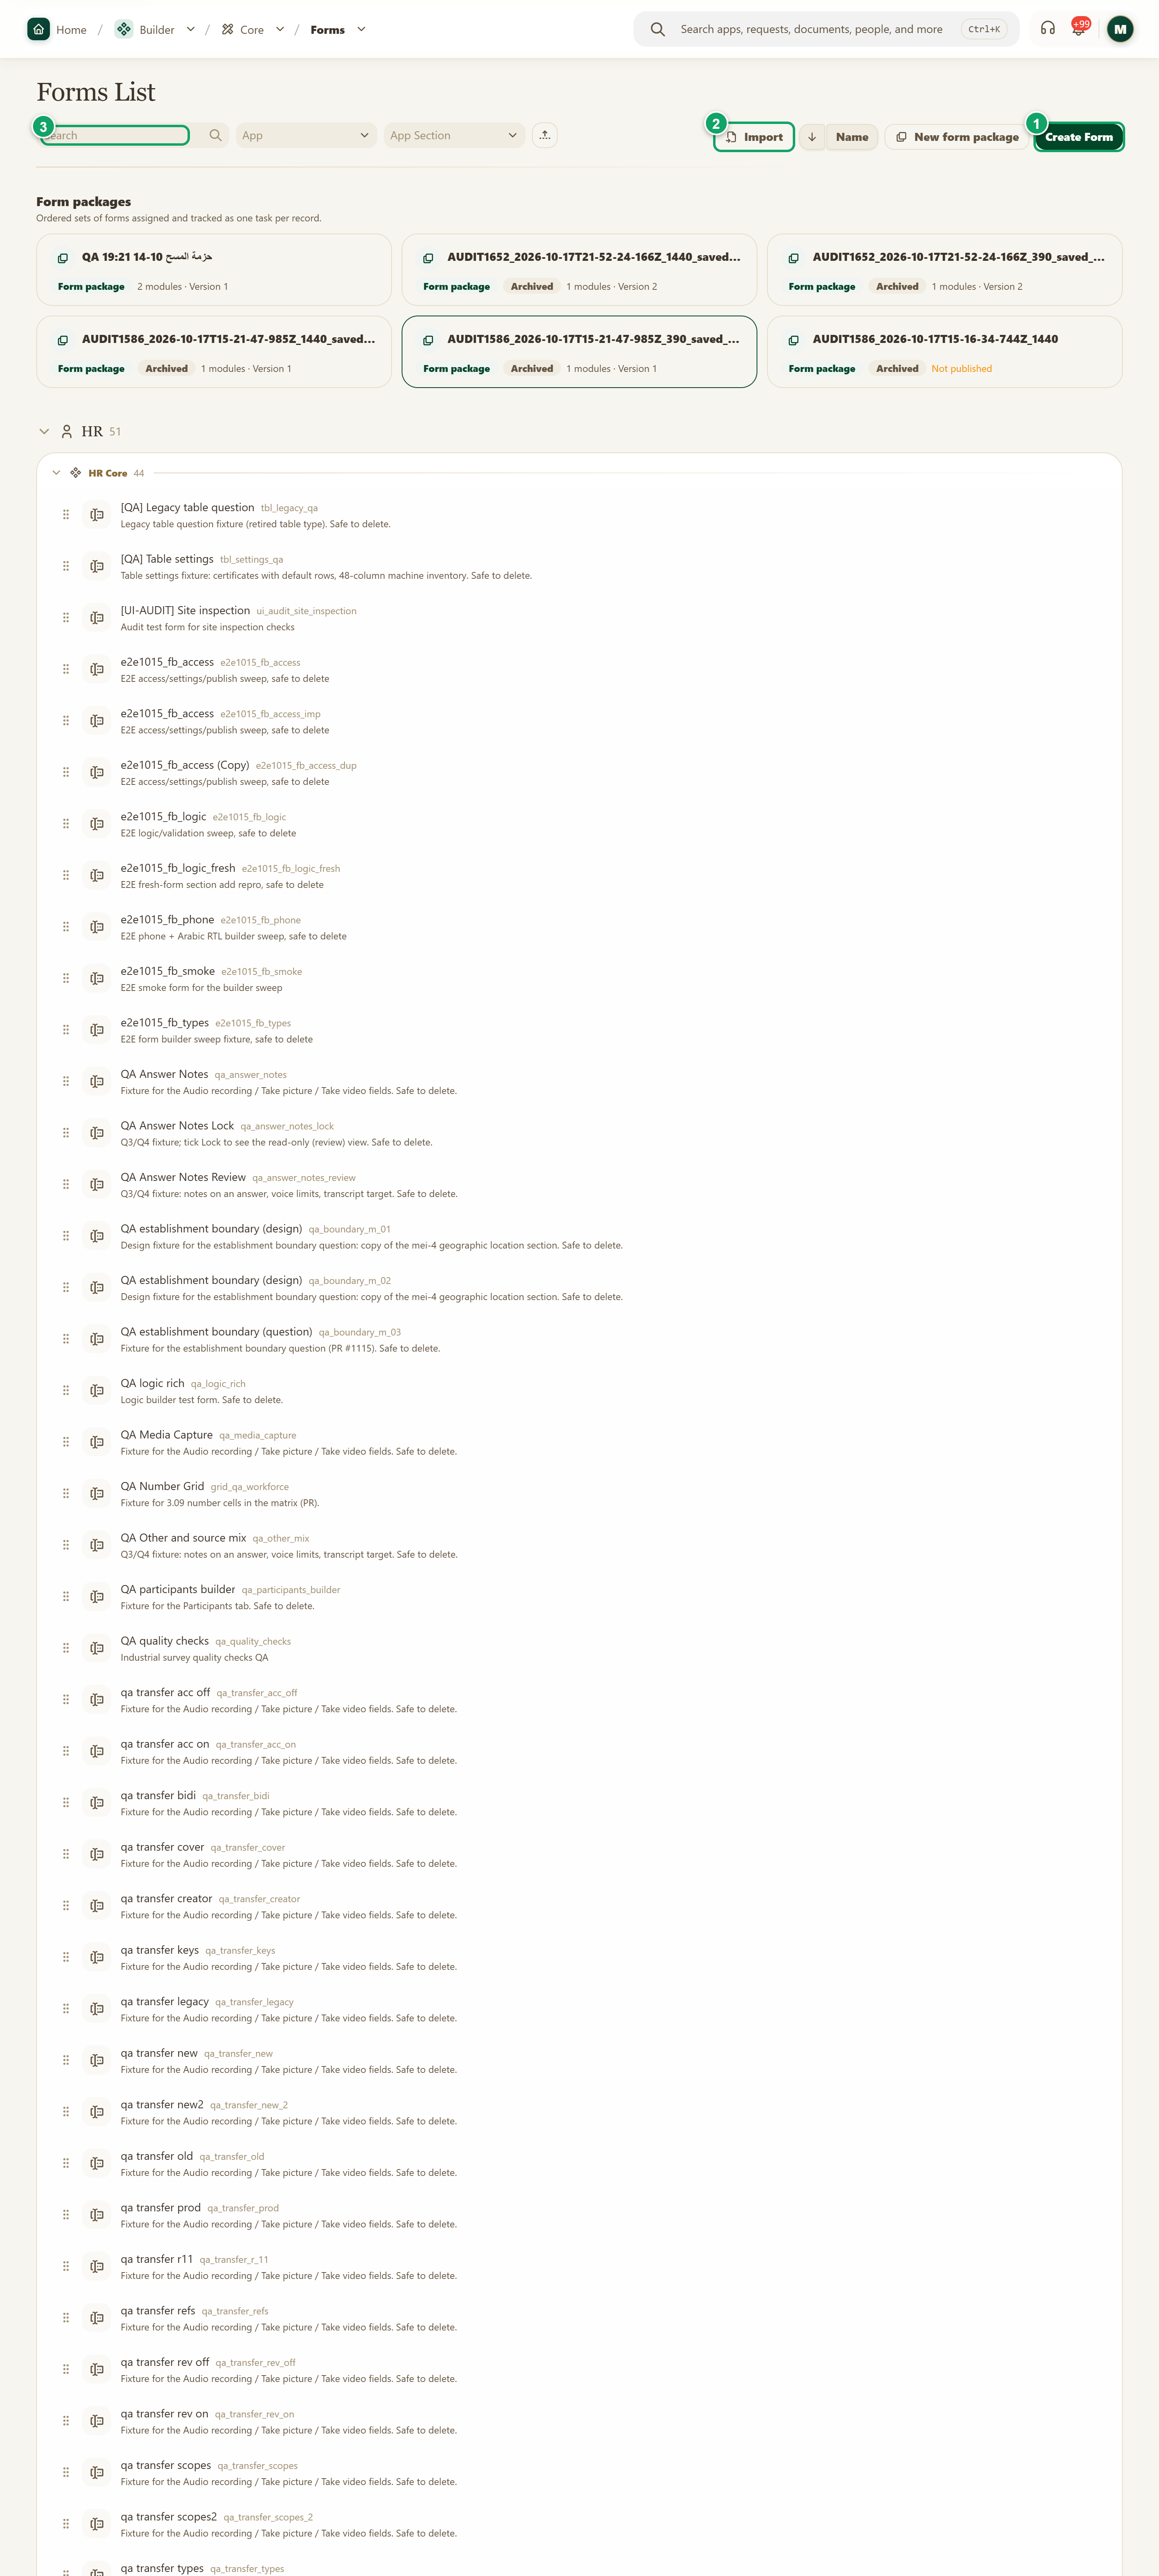
\includegraphics[width=0.95\linewidth,height=0.72\textheight,keepaspectratio]{figures/screens/ch06-forms-en.png}
\caption{The “Forms” page}
\label{fig:builder-forms-screen}
\shotnote{The page lists forms grouped by app and section, with the submission count of each. The forms shown are test forms on test2. ① “Create Form”: starts a new form. ② “Import”: creates a form from an exported file. ③ Search: finds a form by name.}
\end{figure}


\begin{table}[H]
\centering
\caption{The forms list}
\label{tab:builder-forms-list}
\begin{tabularx}{\linewidth}{R{3.6cm} Y}
\rcHeaderRow
\thh{Part} & \thh{Content and action}\\
Create Form & Asks for “Form Name”, “Form Code”, “Reference Prefix”, the app and the section, then opens the builder.\\
The list & Forms grouped by app and section, with search, sorting and submission counts, and the actions “Duplicate”, “Export form” and “Delete Form”.\\
Import & Creates a form from a previously exported file.\\
Form packages & Ordered sets of forms assigned and tracked as one task per record.\\
\end{tabularx}
\end{table}

\begin{table}[H]
\centering
\caption{The form builder's tools}
\label{tab:builder-forms-editor}
\begin{tabularx}{\linewidth}{R{3.6cm} Y}
\rcHeaderRow
\thh{Tool} & \thh{What does it do?}\\
Questions & Adds questions from groups: Text, Choice, Numbers and rating, Date and time, Place, Files \& media, and Other; plus sections, pages and text blocks.\\
Rules & Everything that shows, hides, locks, requires, calculates or checks a question, in one list.\\
Access & Who can reach each response and what they can do with it: the person who starts it, fixed people, or people chosen by the answers.\\
Journey & “Request journey”: the statuses and phases the applicant sees, the transitions between them, and approval steps.\\
Records & The records this form reads from and writes to, and when it writes: “When approved” or “When submitted”.\\
Assign & Plans that assign people to fill the form for certain records; available after the form is saved.\\
Versions and Settings & “Version history” for every version, and settings such as numbering, the PDF document and prefilled links.\\
Test form and Publish & Opens an isolated test workspace where you try the form as a member, then “Publish” makes the draft the live version.\\
\end{tabularx}
\end{table}

\begin{figure}[H]
\centering
\begin{tikzpicture}[node distance=0.5cm]
\node[stepBox] (a) {Create Form};
\node[stepBox,below=of a] (b) {Questions and rules};
\node[stepBox,below=of b] (c) {Access, journey, records};
\node[stepBox,below=of c] (d) {Test form};
\node[stepBox,below=of d] (e) {Publish};
\draw[flowsTo] (a) -- (b);
\draw[flowsTo] (b) -- (c);
\draw[flowsTo] (c) -- (d);
\draw[flowsTo] (d) -- (e);
\end{tikzpicture}
\rclegend
\caption{From idea to published form}
\label{fig:builder-forms-flow}
\shotnote{The diagram orders form building from content to behaviour: questions first, then who reaches the response and where the answers go. Testing comes before publishing because the test workspace is isolated, so it exposes mistakes without reaching anyone; publishing makes the version available to everyone who fills in the form.}
\end{figure}

\subsection{Steps and check}
\begin{enumerate}
\item Open “Forms” and press “Create Form”, then write the name, code and prefix and choose the app and section.
\item Add the questions, choosing a type that fits each answer, then add rules when needed.
\item Open “Access” to decide who sees responses, and “Records” if the answers should be written into a record type.
\item Press “Test form” and fill it in completely, then press “Publish”.
\end{enumerate}

\textbf{Check and recovery:} the message “Form published successfully” should appear, and the version should show as live in “Version history”. If the publish button turns into “Send for approval”, your organization requires publishing approval, and the form goes live after the approver agrees. If answers are not written to the record, open “Records” and check that the record type's administrator has allowed the form to write there.

\clearpage
\section{Services}
\label{sec:builder-feature-services}

A service is what the public sees on the organization's portal, such as “Certificate request” or “Book an appointment”. Each service holds one or more forms and decides how it is delivered and who may apply. So a form reaches applicants only through a service; a form that belongs to no service stays an “internal form” for staff only.

\textbf{Path and who uses it:} “Builder” → “Core” → “Services”. Used by those who manage the organization's public services.

\begin{rcnote}[Example: Horizon]
Horizon accepts maintenance requests from its Aleppo customers, so the system administrator creates a “Maintenance request” service that starts with a published form and makes it available to registered accounts only. The “Branch visit request” form stays an internal form. They start the service from ①, and the visit form stays in ④.
\end{rcnote}

\begin{figure}[H]
\centering
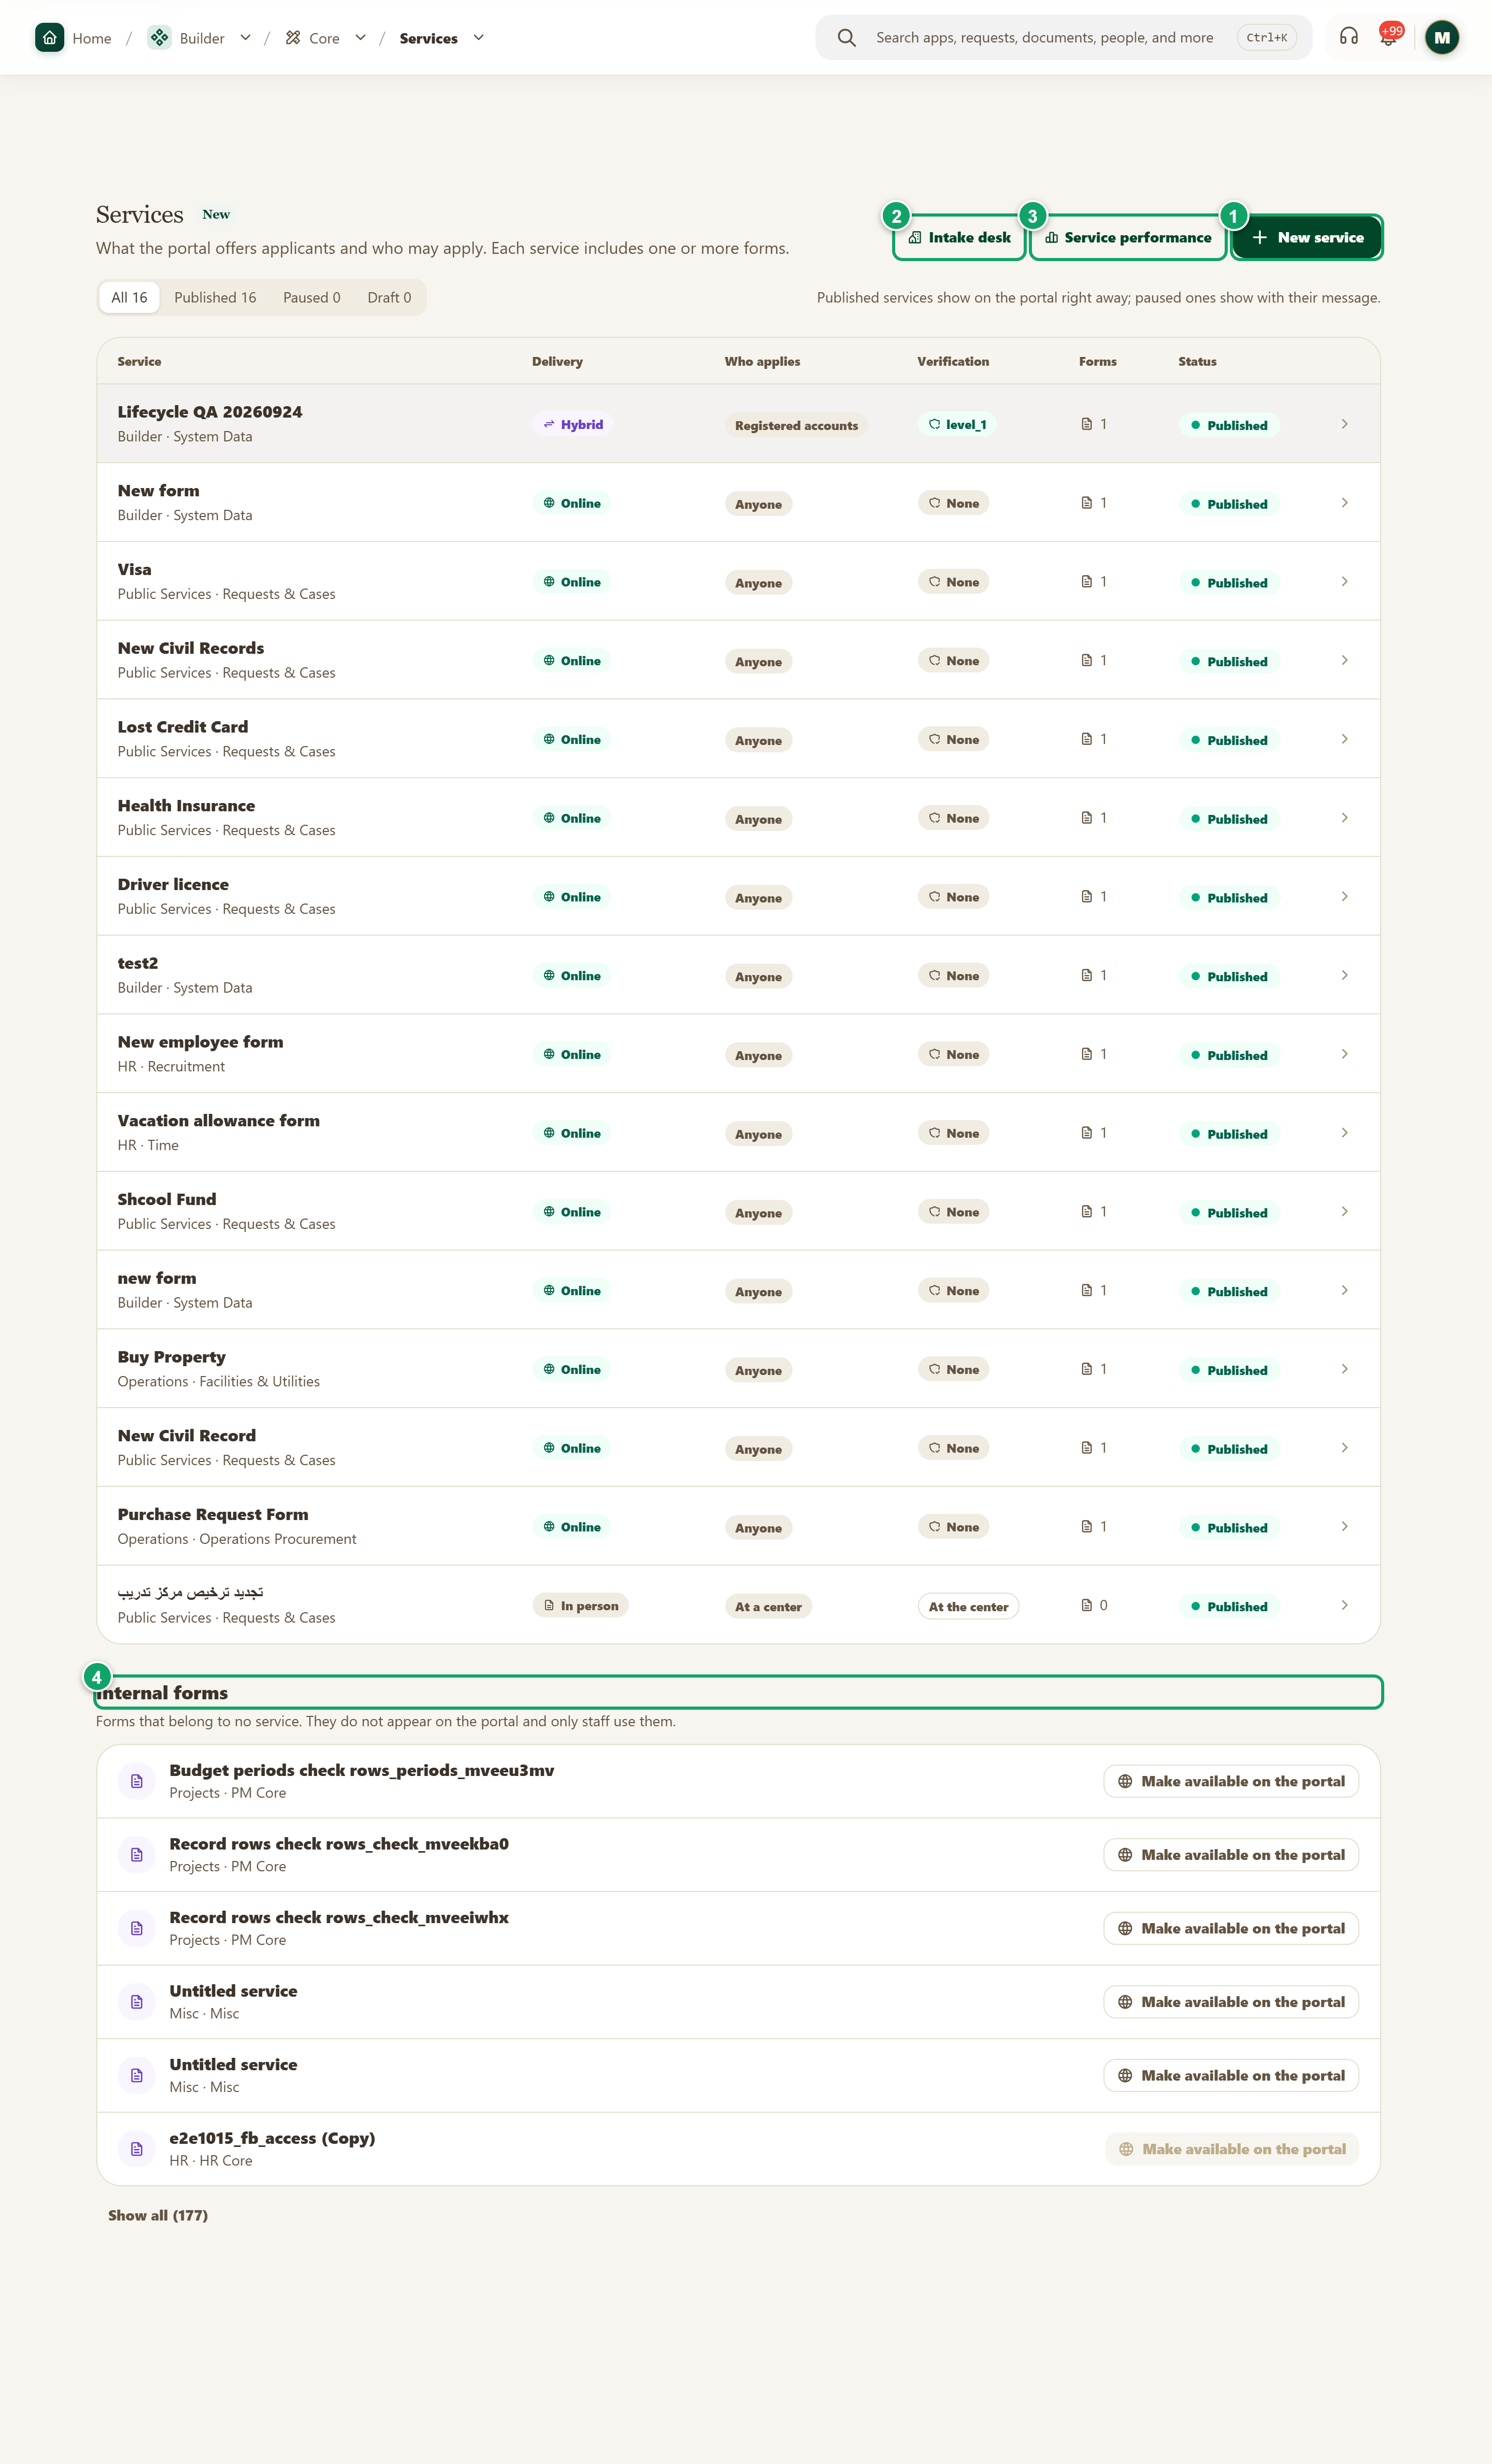
\includegraphics[width=0.95\linewidth,height=0.72\textheight,keepaspectratio]{figures/screens/ch06-services-en.png}
\caption{The “Services” page}
\label{fig:builder-services-screen}
\shotnote{The page lists the services shown on the portal and their state, then the internal forms that belong to no service. ① “New service”: starts a service around a published form. ② “Intake desk”: registers an in-person request. ③ “Service performance”: shows how requests move. ④ “Internal forms”: forms the public does not see.}
\end{figure}


\begin{table}[H]
\centering
\caption{What do you find here?}
\label{tab:builder-services-data}
\begin{tabularx}{\linewidth}{R{3.6cm} Y}
\rcHeaderRow
\thh{Part} & \thh{Content and action}\\
Services & The services table with “Delivery”, “Who applies”, “Verification”, forms and status, filtered by “Published”, “Paused” or “Draft”.\\
New service & Asks for the service name and the “Form the applicant starts with”, plus an optional staff record form.\\
Internal forms & Forms that belong to no service. “Make available on the portal” turns a published form into a new service or a step in an existing one.\\
Service page & Tabs “Overview”, “Fees”, “Profile”, “Delivery \& eligibility” and “Path \& forms”.\\
Intake desk and Service performance & Register an in-person request at a service center, and follow how requests move and where they wait.\\
\end{tabularx}
\end{table}

\begin{figure}[H]
\centering
\begin{tikzpicture}[node distance=0.5cm]
\node[entity] (service) {Service};
\node[entity,below right=0.7cm and 0.3cm of service] (entry) {Starting form};
\node[entityOpt,below left=0.7cm and 0.3cm of service] (more) {Path and follow-up forms};
\draw[dependsOn] (service.south) -- ++(0,-0.3) -| (entry.north);
\draw[dependsOnOpt] (service.south) -- ++(0,-0.3) -| (more.north);
\end{tikzpicture}
\rclegend
\caption{What a service holds}
\label{fig:builder-services-model}
\shotnote{The figure shows that a service needs a published starting form the applicant fills in, while the other forms are optional, such as later path steps or a follow-up form requested at a given status. So publish the form in the form builder first, then build the service around it.}
\end{figure}

\subsection{Steps and check}
\begin{enumerate}
\item Publish the form the applicant will start with on the “Forms” page.
\item Open “Services”, press “New service”, choose the form, then press “Create service”.
\item Complete the “Profile” the applicant reads, and set who may apply under “Delivery \& eligibility”.
\item Publish the service, then press “View on portal” to see it as the applicant does.
\end{enumerate}

\textbf{Check and recovery:} a published service should appear on the portal right away. If it does not, make sure it is not a “Draft”, because “Drafts are not on the portal”. To stop requests for a while, set it to “Paused” with a message to applicants instead of deleting it.

\clearpage
\section{Internal SOPs}
\label{sec:builder-feature-internal-sops}

An internal SOP is a workflow that starts on an event you choose and then runs steps in order: a human step such as an approval, signature or task, or an automatic step such as creating a record or sending a notification. You build, test and publish SOPs on this page without external tools.

\textbf{Path and who uses it:} “Builder” → “Core” → “Internal SOPs”. Used by those who design the organization's workflows.

\begin{rcnote}[Example: Horizon]
The system administrator builds an “Approve visit request” SOP that starts “On Form Submitted” for the visit request form, sends an “Approval Request” to Sarah Al-Khatib, then creates a task for Omar Haddad to prepare the visit if she approves. The SOP starts from ① and is followed in ②.
\end{rcnote}

\begin{figure}[H]
\centering
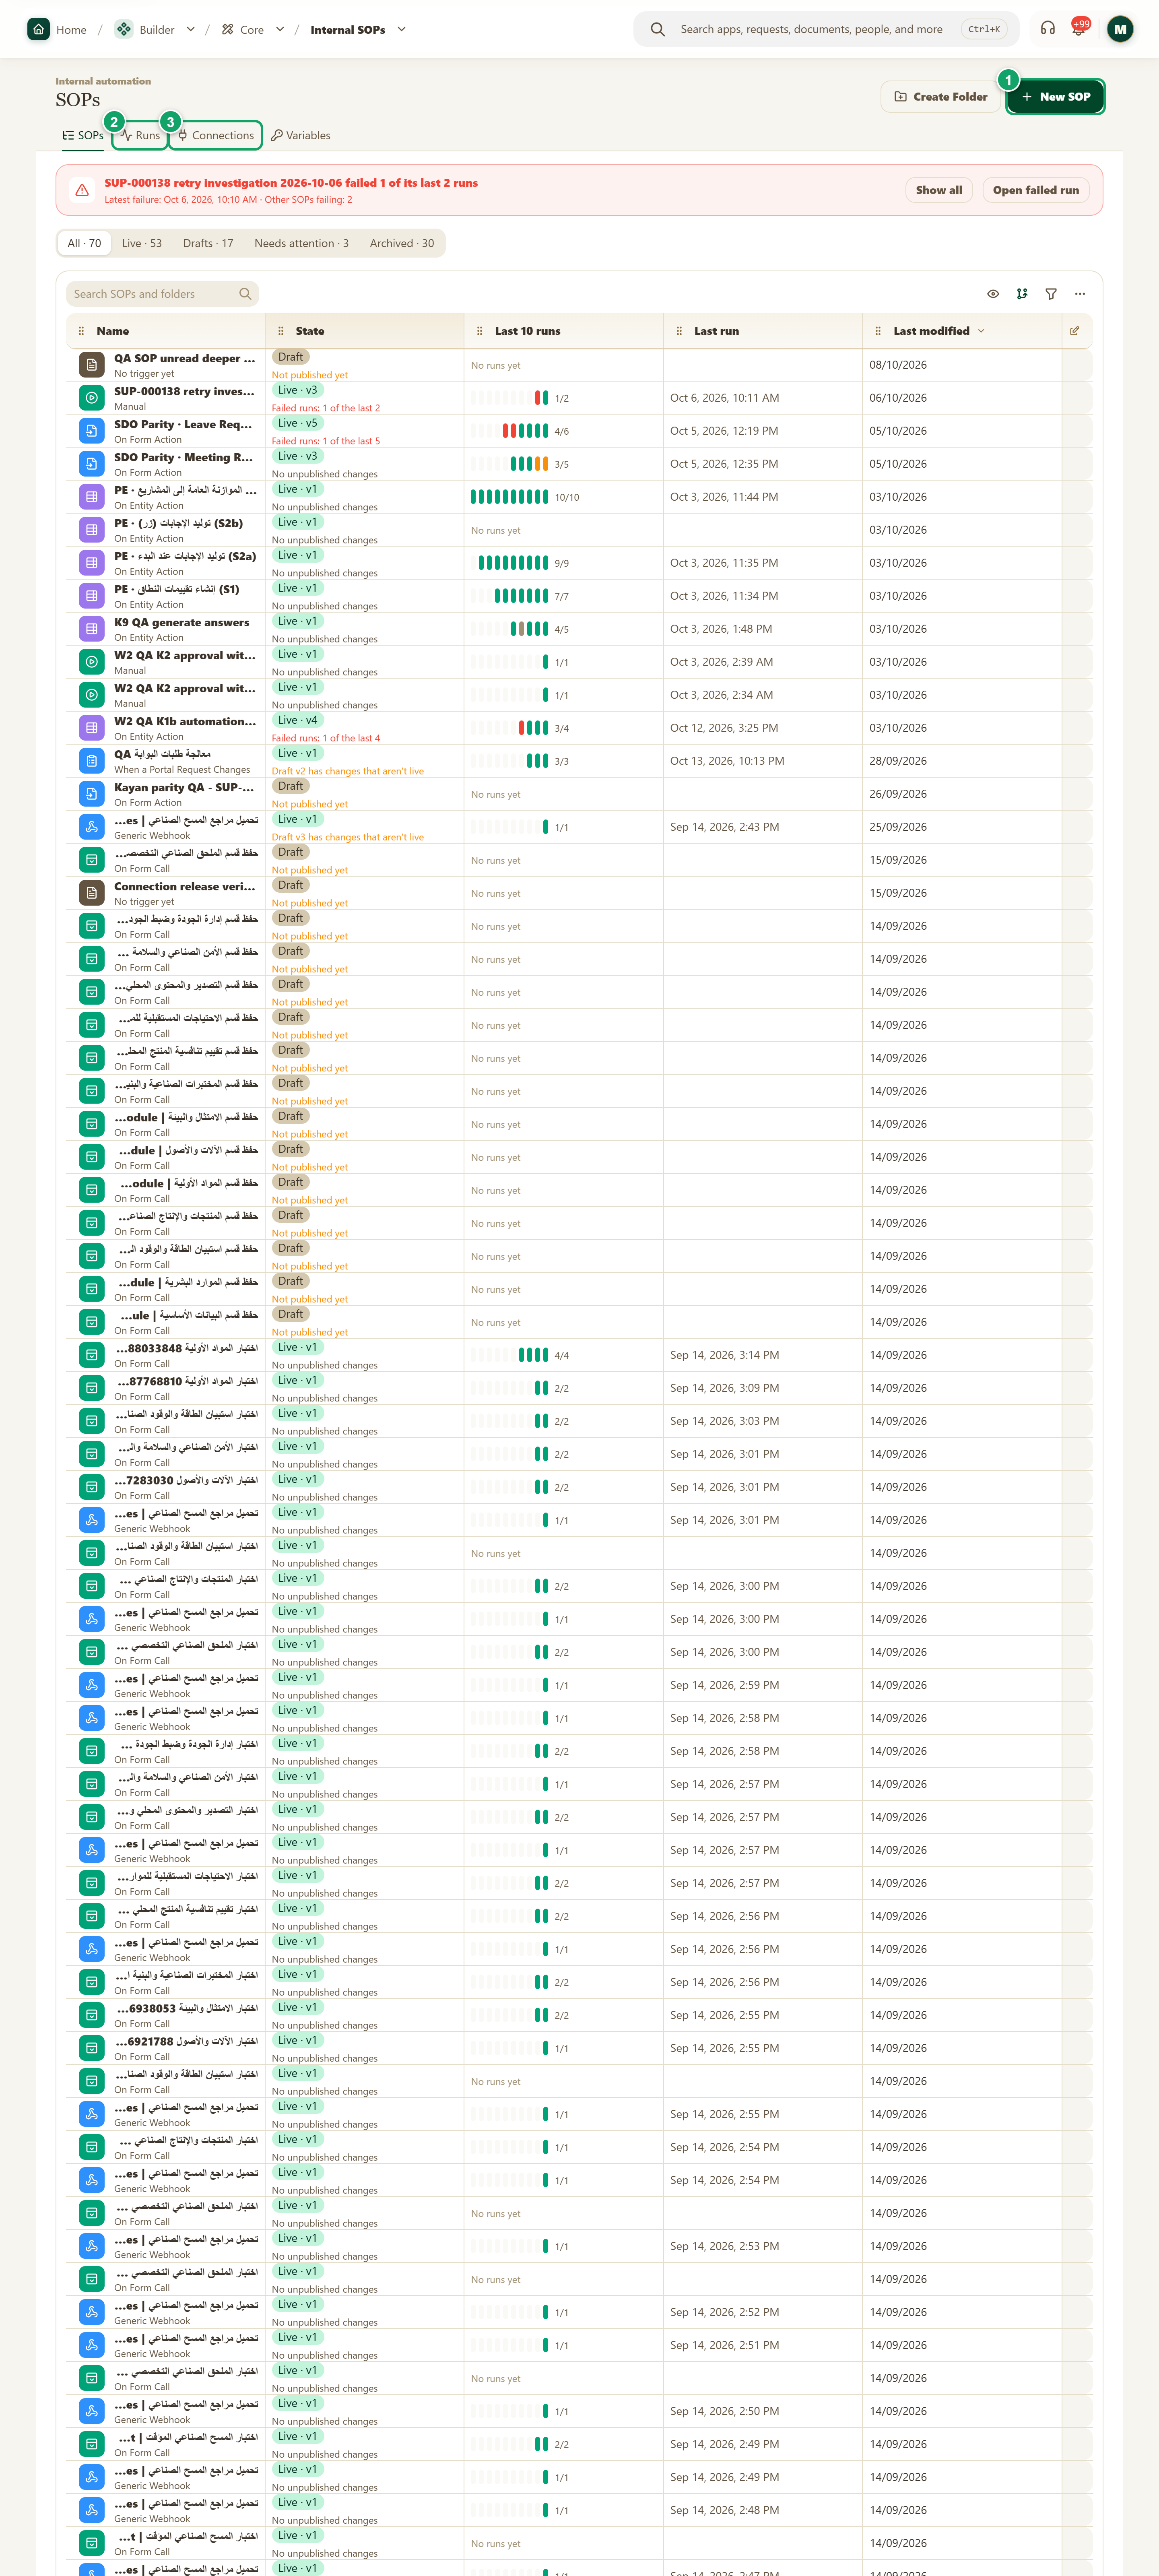
\includegraphics[width=0.95\linewidth,height=0.72\textheight,keepaspectratio]{figures/screens/ch06-internal-sops-en.png}
\caption{The “Internal SOPs” page}
\label{fig:builder-internal-sops-screen}
\shotnote{The page lists SOPs, their states and follow-up tabs. The list is empty in the test organization. ① “New SOP”: starts an SOP and asks what starts it. ② “Runs”: every time an SOP ran and its result. ③ “Connections”: external service accounts the steps use.}
\end{figure}


\begin{table}[H]
\centering
\caption{What do you find here?}
\label{tab:builder-internal-sops-data}
\begin{tabularx}{\linewidth}{R{3.6cm} Y}
\rcHeaderRow
\thh{Tab or tool} & \thh{Content and action}\\
SOPs & The list of SOPs with their state and recent run results, filtered by “Live”, “Drafts”, “Needs attention”, “Paused” and “Archived”.\\
Runs & Every time an SOP started, with its status: queued, running, waiting, completed or failed.\\
Connections and Variables & External service accounts the steps use, and encrypted values SOPs can use.\\
New SOP & Write the name and choose “What starts it?”, such as “On Form Submitted”, “New Record Created”, “Schedule” or “Manual”, then “Create and open”.\\
Editor & The step canvas with “Build”, “Test” and “Runs” modes. Steps include approval, form and signature requests, task creation, decisions, waits, and creating or updating records.\\
Review \& publish & Shows what to fix and the changes since the live version, then publishes a new version. Runs in progress finish on their old version.\\
\end{tabularx}
\end{table}

\begin{figure}[H]
\centering
\begin{tikzpicture}[node distance=0.5cm]
\node[stepBox] (a) {Trigger: what starts it?};
\node[stepBox,below=of a] (b) {Human and automatic steps};
\node[stepBox,below=of b] (c) {Test: safe simulation};
\node[stepBox,below=of c] (d) {Review and publish};
\node[stepBox,below=of d] (e) {Follow the runs};
\draw[flowsTo] (a) -- (b);
\draw[flowsTo] (b) -- (c);
\draw[flowsTo] (c) -- (d);
\draw[flowsTo] (d) -- (e);
\end{tikzpicture}
\rclegend
\caption{The life of an internal SOP}
\label{fig:builder-internal-sops-flow}
\shotnote{The diagram shows that an SOP runs only after it is published, and that testing comes before publishing. “Simulate (safe)” creates nothing real and makes external steps return example data, so you test the path without disturbing anyone. After publishing, follow the runs to see where the SOP succeeded and where it stopped.}
\end{figure}

\subsection{Steps and check}
\begin{enumerate}
\item Open “Internal SOPs”, press “New SOP”, name it, choose what starts it and press “Create and open”.
\item Add the steps on the canvas and finish setting up each one until “All steps ready” appears.
\item Switch to “Test” mode, choose “Simulate (safe)”, then press “Run simulation”.
\item Press “Review \& publish”, review the changes, then publish the version.
\end{enumerate}

\textbf{Check and recovery:} the SOP's state should be “Live”, and runs should appear after the event happens. If a run fails, open it from “Runs” to see the failed step, fix it and publish again. To stop the SOP for a while, pause it instead of deleting it; no new runs start until you resume it.

\clearpage
\section{SOPs}
\label{sec:builder-feature-sops}

This page opens an embedded automation studio that builds flows connecting KayanOS with other accounts and services, starting on a KayanOS event such as a record being created or a form being submitted. Every automation in it works through a KayanOS account connection you choose first. For approval and task workflows inside the organization, “Internal SOPs” is the better fit.

\textbf{Path and who uses it:} “Builder” → “Core” → “SOPs”. Used by those with forms permission who need to connect KayanOS with other systems.

\begin{rcnote}[Example: Horizon]
Horizon wants a message to reach an external tracking sheet whenever a visit request is created. So the system administrator builds an automation that starts when a new record is created in “Visit requests”, then checks the branch before sending the data.
\end{rcnote}

\begin{table}[H]
\centering
\caption{The parts of an automation}
\label{tab:builder-sops-parts}
\begin{tabularx}{\linewidth}{R{3.6cm} Y}
\rcHeaderRow
\thh{Part} & \thh{Meaning}\\
Connection & The KayanOS account the automation acts as, chosen first. Give it only the permissions the work needs.\\
Trigger & The event that starts the automation, such as a record created or updated, or an action on a form or task.\\
Condition & Checks the data before any write, so the automation does not act on records that are not its concern.\\
Actions & What the automation does: create, update or find records, create tasks, send a notification and more.\\
\end{tabularx}
\end{table}

\begin{figure}[H]
\centering
\begin{tikzpicture}[node distance=0.5cm]
\node[stepBox] (a) {Choose the connection};
\node[stepBox,below=of a] (b) {Trigger};
\node[stepBox,below=of b] (c) {Condition before writing};
\node[stepBox,below=of c] (d) {One action at a time};
\draw[flowsTo] (a) -- (b);
\draw[flowsTo] (b) -- (c);
\draw[flowsTo] (c) -- (d);
\end{tikzpicture}
\rclegend
\caption{The order for building an automation}
\label{fig:builder-sops-flow}
\shotnote{The diagram puts the condition before the action, because an automation that writes without checking can change many records in a moment. Test the parts one by one: the trigger alone, then the condition both ways, then each action separately.}
\end{figure}

\subsection{Steps and check}
\begin{enumerate}
\item Open “SOPs”, create a new flow, then choose a KayanOS connection.
\item Choose the trigger and test it with sample data.
\item Add a condition that checks the data, then add the actions one after another, testing each one.
\item Turn the automation on after the tests pass, then review the first real run.
\end{enumerate}

\textbf{Check and recovery:} the run should appear in the automation's history with the expected result. If the page stays empty or shows an error, the automation service may not be available in your organization's environment; on the \en{test2} test environment the page was empty when checked. If an action fails, check the connection's permissions first.

\clearpage
\section{Bots}
\label{sec:builder-feature-bots}

A bot is an assistant with a name and picture that members add to chat, email or calendar. On this page you decide where it can be added, whether it is added automatically, and how it reaches email. What the bot does when messaged or mentioned is built in “Internal SOPs” with triggers such as “On Direct Message to Bot” and “On Mention”.

\textbf{Path and who uses it:} “Builder” → “Core” → “Bots”. Used by those with bots permission.

\begin{rcnote}[Example: Horizon]
The system administrator creates a “Visits assistant” bot and makes it addable to direct chats. When Omar Haddad messages it, an internal SOP starts and replies with the status of his visit request. The bot starts from ①.
\end{rcnote}

\begin{figure}[H]
\centering
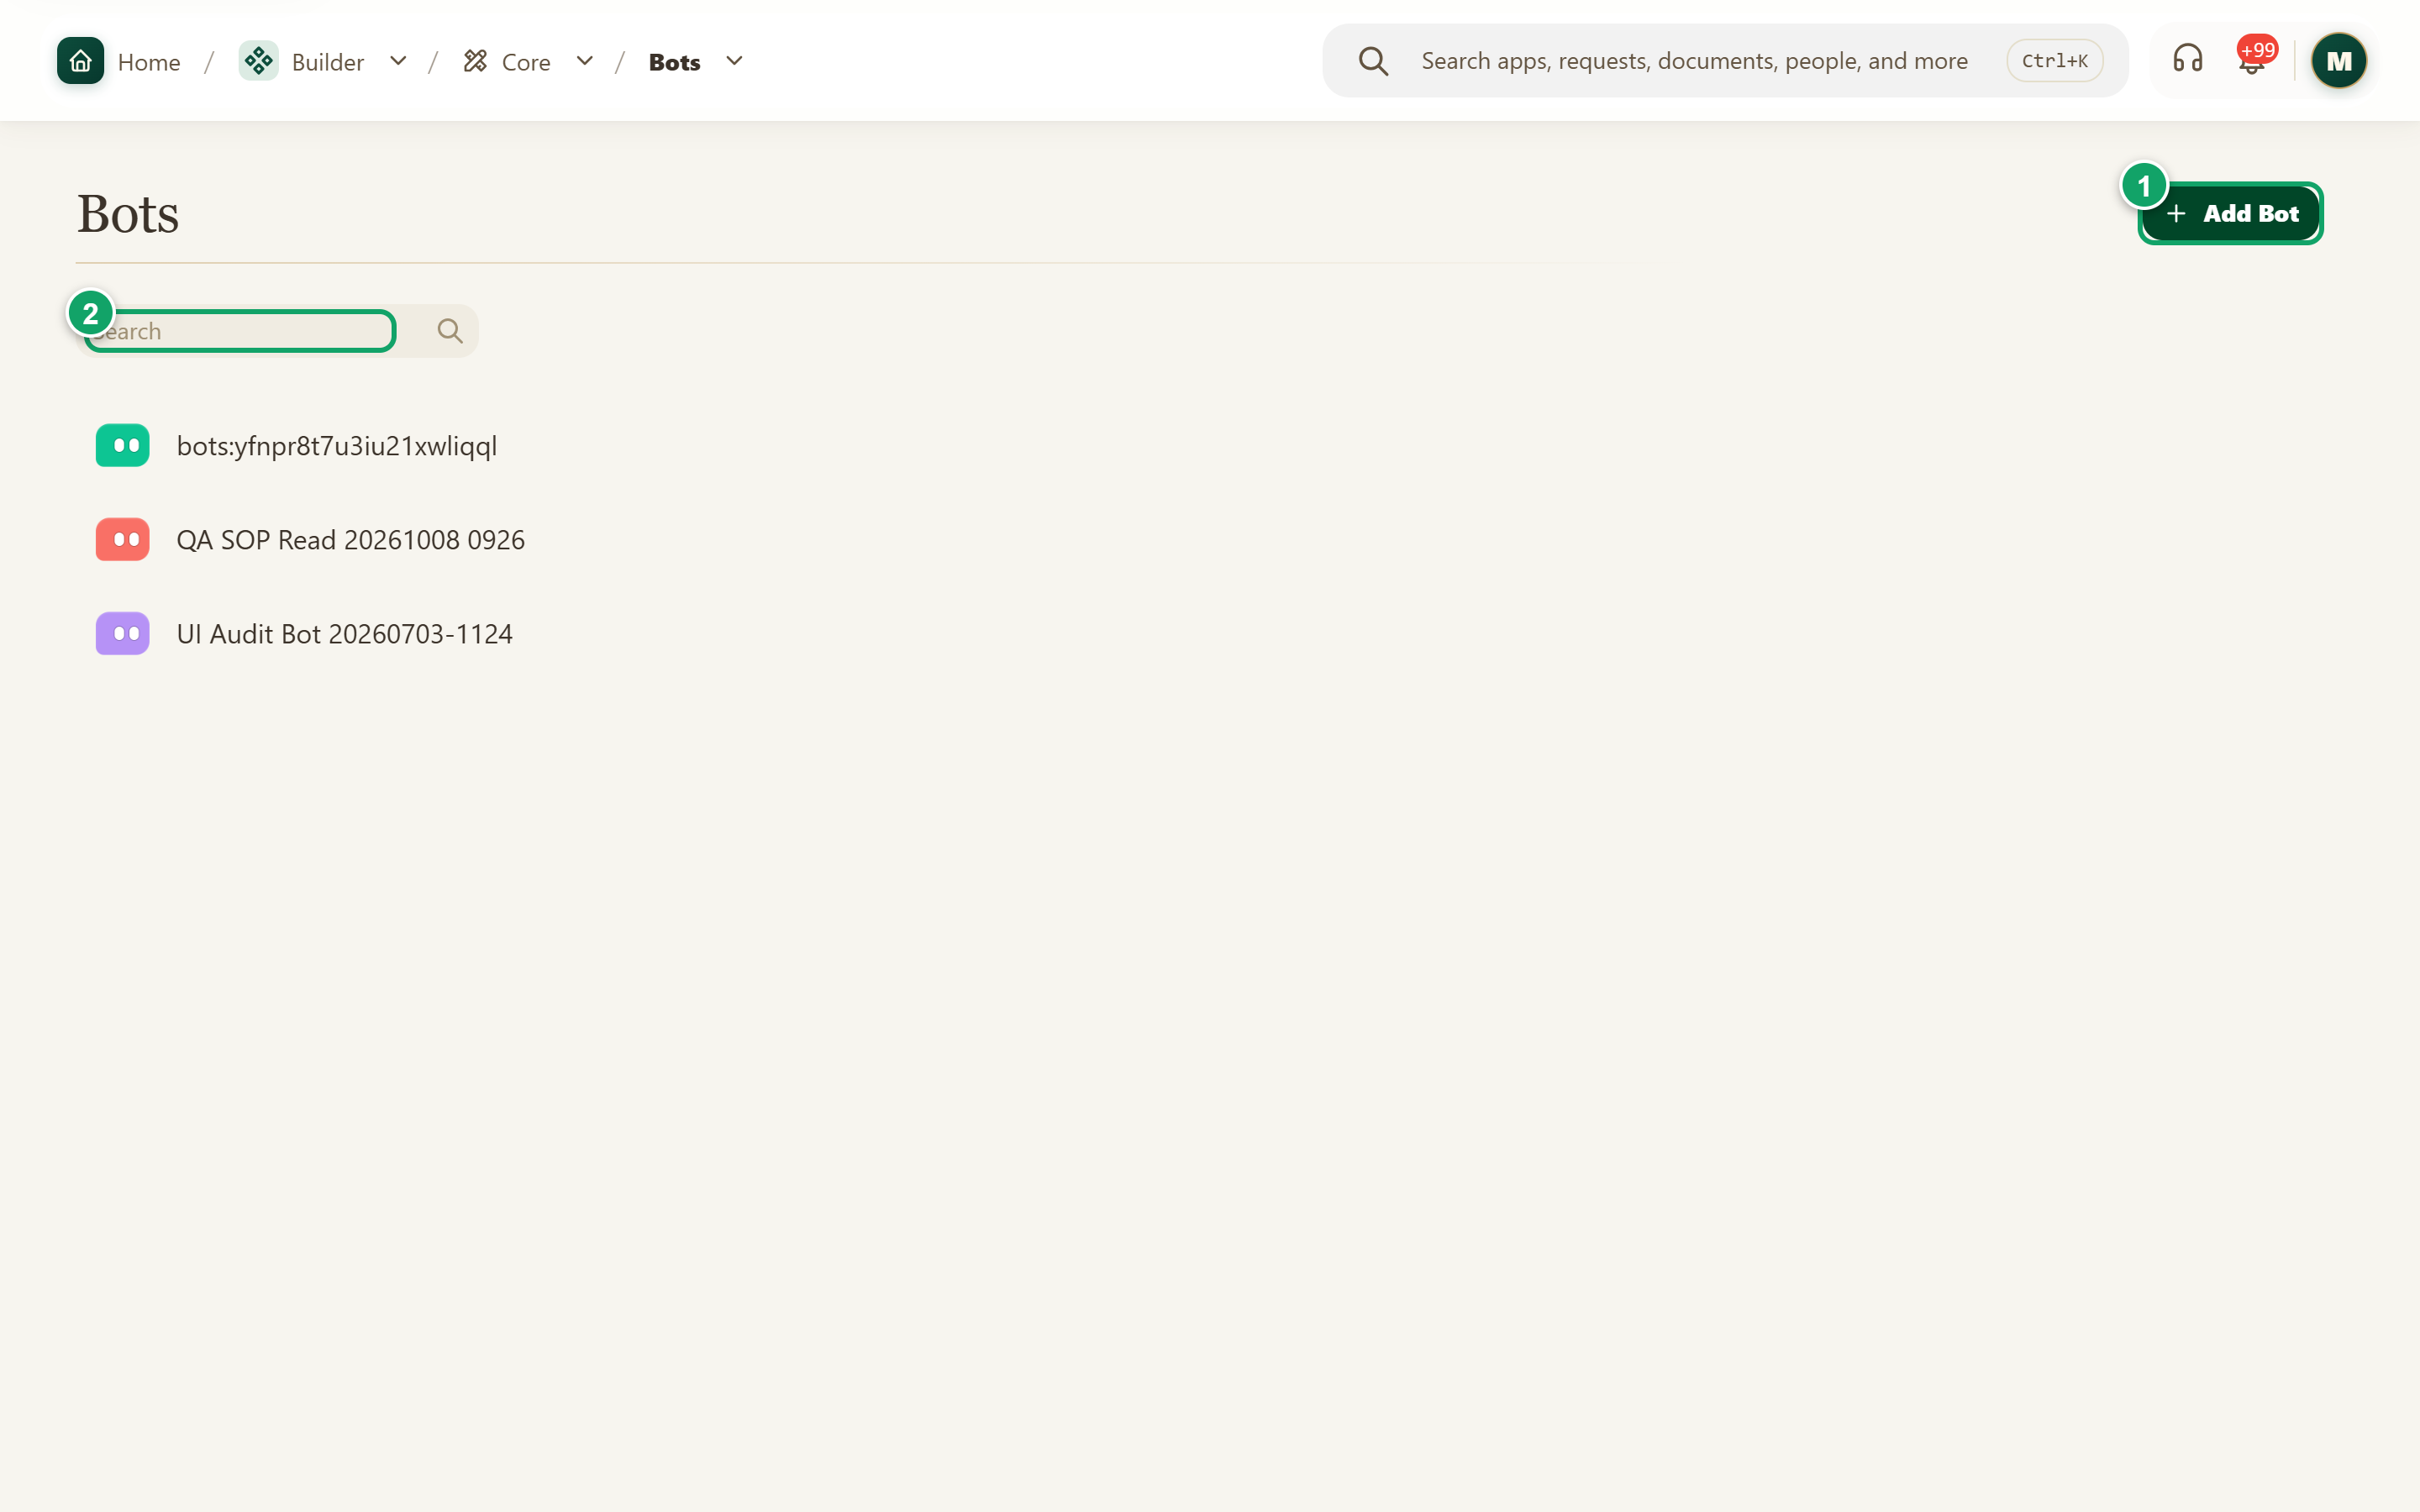
\includegraphics[width=0.95\linewidth,height=0.72\textheight,keepaspectratio]{figures/screens/ch06-bots-en.png}
\caption{The “Bots” page}
\label{fig:builder-bots-screen}
\shotnote{The page lists the organization’s bots, here test bots. ① “Add Bot”: asks only for a name. ② Search: finds a bot by name.}
\end{figure}


\begin{table}[H]
\centering
\caption{Bot settings}
\label{tab:builder-bots-data}
\begin{tabularx}{\linewidth}{R{3.6cm} Y}
\rcHeaderRow
\thh{Section} & \thh{What do you set?}\\
Add Bot & Asks only for the name; the picture is chosen automatically.\\
Chat & Whether it can be added to direct chats or channels, and whether it can be messaged or mentioned.\\
Emails & Whether it is installable in email, can be CCed, and can add internal or external contacts.\\
Calendar & Whether it can be installed in the calendar.\\
Default installation & Whether it is added automatically to chat, email or calendar, and its default email access.\\
\end{tabularx}
\end{table}

\begin{figure}[H]
\centering
\begin{tikzpicture}[node distance=0.5cm]
\node[entity] (bot) {Bot};
\node[entityOpt,below right=0.7cm and 0.3cm of bot] (where) {Where it is added};
\node[entityOpt,below left=0.7cm and 0.3cm of bot] (sop) {Internal SOP that replies};
\draw[dependsOnOpt] (bot.south) -- ++(0,-0.3) -| (where.north);
\draw[dependsOnOpt] (bot.south) -- ++(0,-0.3) -| (sop.north);
\end{tikzpicture}
\rclegend
\caption{The bot's identity and its work}
\label{fig:builder-bots-model}
\shotnote{The figure separates two things: this page sets the bot's identity and where it can be added, while its replies come from an internal SOP that starts when the bot is messaged or mentioned. So a bot does nothing on its own until you connect it to a published SOP.}
\end{figure}

\subsection{Steps and check}
\begin{enumerate}
\item Open “Bots”, press “Add Bot”, write the name and press “Create”.
\item Open the bot, turn on where it can be added in chat, email and calendar, then press “Save”.
\item In “Internal SOPs”, build an SOP that starts “On Direct Message to Bot” and publish it.
\end{enumerate}

\textbf{Check and recovery:} add the bot to a test chat and message it; the SOP should start and appear under “Runs”. If members do not see the option to add it, review the chat settings and save; if the bot does not reply, make sure the SOP is published and not paused.

\clearpage
\section{DOCX Templates}
\label{sec:builder-feature-docx-templates}

A DOCX template is an ordinary Word file where you write the fixed text and put tags in double braces where variable data goes, such as the employee's name or the request number. When a user presses the action button on a record, KayanOS fills the tags from the record's data and downloads the document as Word or PDF. That way contracts and letters are produced with consistent wording and no manual copying.

\textbf{Path and who uses it:} “Builder” → “Core” → “DOCX Templates”. Managed by those with Builder administration; users run them from a button on the record.

\begin{rcnote}[Example: Horizon]
The system administrator writes the visit confirmation letter in Word, adds one tag for the request number and another for the visit date, uploads it as a template and links it to a button in “Visit requests”. They upload the letter from ① and test it after opening it from ③.
\end{rcnote}

\begin{figure}[H]
\centering
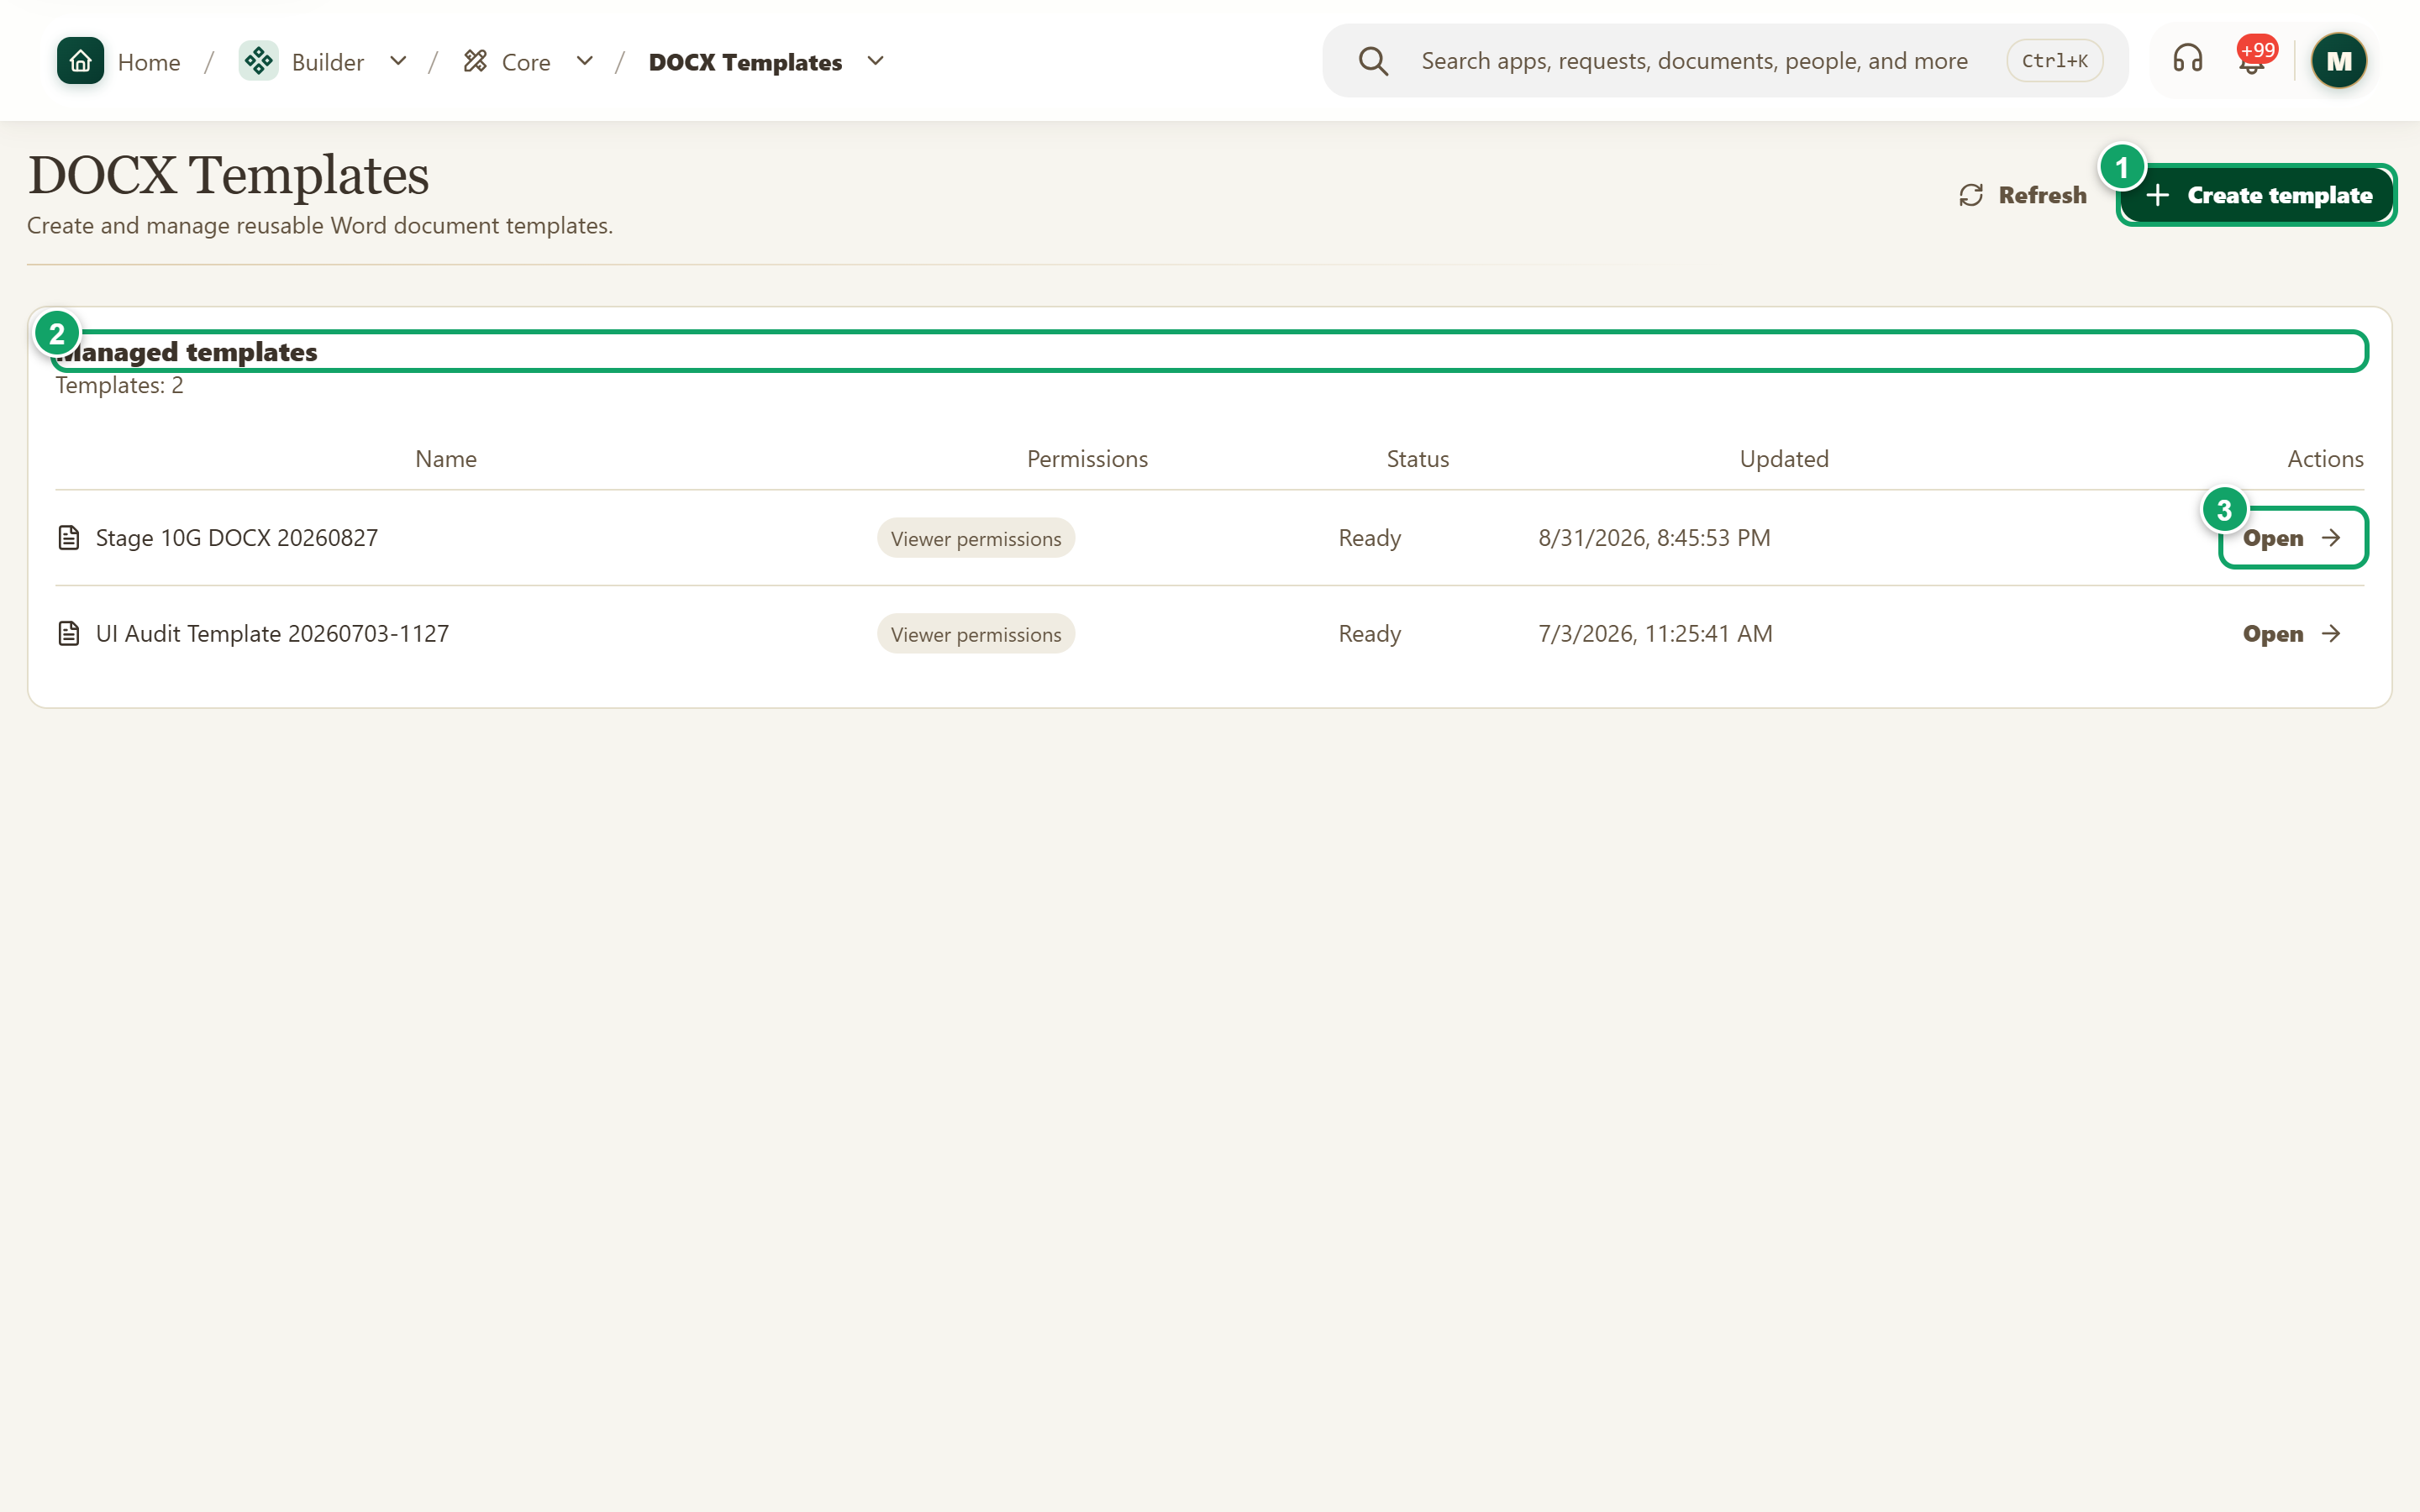
\includegraphics[width=0.95\linewidth,height=0.72\textheight,keepaspectratio]{figures/screens/ch06-docx-en.png}
\caption{The “DOCX Templates” page}
\label{fig:builder-docx-templates-screen}
\shotnote{The page lists managed templates with their permissions and status, here test templates. ① “Create template”: uploads a new Word file. ② “Managed templates”: the list with each template’s status. ③ “Open”: opens a template for settings, versions and testing.}
\end{figure}


\begin{table}[H]
\centering
\caption{What do you find here?}
\label{tab:builder-docx-data}
\begin{tabularx}{\linewidth}{R{3.6cm} Y}
\rcHeaderRow
\thh{Part} & \thh{Content and action}\\
Managed templates & The list of templates with “Permissions” and “Status”: “Ready” when a current version exists, or “Needs a Word document”.\\
Create template & Upload a “Word document” and write the “Template name”; you can also set the downloaded file name and the document permissions.\\
Document permissions & “Viewer permissions”, the recommended choice, show only what the downloader can see. “Administrator permissions” may put data in the document they cannot view.\\
Settings and Versions & Edit the settings, upload a new version after it is validated, and review “Version history”.\\
Test \& download & Choose a real record and Word or PDF, then “Render and download” to see the result before anyone uses it.\\
\end{tabularx}
\end{table}

\begin{table}[H]
\centering
\caption{Tag examples}
\label{tab:builder-docx-tags}
\begin{tabularx}{\linewidth}{R{3.6cm} Y}
\rcHeaderRow
\thh{Tag} & \thh{What does it do?}\\
\en{\{\{ \$record.field\_key \}\}} & Inserts a field value from the record, using the field's key, not its label.\\
\en{\{\{\#if ...\}\}} & Shows a paragraph when a condition is met, and ends with \en{\{\{/if\}\}}.\\
\en{\{\{\#each ...\}\}} & Repeats a row or paragraph for each item in a list, and ends with \en{\{\{/each\}\}}.\\
\end{tabularx}
\end{table}

\begin{figure}[H]
\centering
\begin{tikzpicture}[node distance=0.5cm]
\node[stepBox] (a) {Word file with tags};
\node[stepBox,below=of a] (b) {Create and test the template};
\node[stepBox,below=of b] (c) {“Word document” action on the record};
\node[stepBox,below=of c] (d) {The user presses the button};
\draw[flowsTo] (a) -- (b);
\draw[flowsTo] (b) -- (c);
\draw[flowsTo] (c) -- (d);
\end{tikzpicture}
\rclegend
\caption{From a Word file to a document for every record}
\label{fig:builder-docx-flow}
\shotnote{The diagram shows that a template is not linked to a record type by itself; it reaches users through a “Word document” action you add in “Actions \& automations”. That is why testing on a real record comes before linking, because validation at upload does not catch every mistake in where tags are placed.}
\end{figure}

\subsection{Steps and check}
\begin{enumerate}
\item Write the document in Word, place tags using the real field keys, and put condition and loop tags in their own paragraph.
\item Open “DOCX Templates” and press “Create template”, upload the file, write the name and press “Create template”.
\item Open “Test \& download”, choose a record, then “Render and download” and review the document.
\item In the record type, add an action of kind “Word document” linked to the template, then publish.
\end{enumerate}

\textbf{Check and recovery:} the template's status should be “Ready”, and the action button should download a document filled with the record's data. If “This document needs attention” appears at upload, fix the listed tags and upload again. If a value is blank, check that you used the field's key, not its label.

\clearpage
\section{XLSX Templates}
\label{sec:builder-feature-xlsx-templates}

An XLSX template is an Excel workbook with tags of the same kind, which KayanOS fills from the record's data and downloads as Excel or PDF. It suits lists and tabular reports with repeating rows, because tags can repeat rows and columns. A tag placed alone in a cell keeps the value's type as a number or date.

\textbf{Path and who uses it:} “Builder” → “Core” → “XLSX Templates”. Managed by those with Builder administration.

\begin{rcnote}[Example: Horizon]
The system administrator prepares a “Branch visits sheet” workbook that repeats a row for each visit, and links it to a “Spreadsheet” button, so Sarah Al-Khatib downloads the sheet ready in Excel. They upload the workbook from ①.
\end{rcnote}

\begin{figure}[H]
\centering
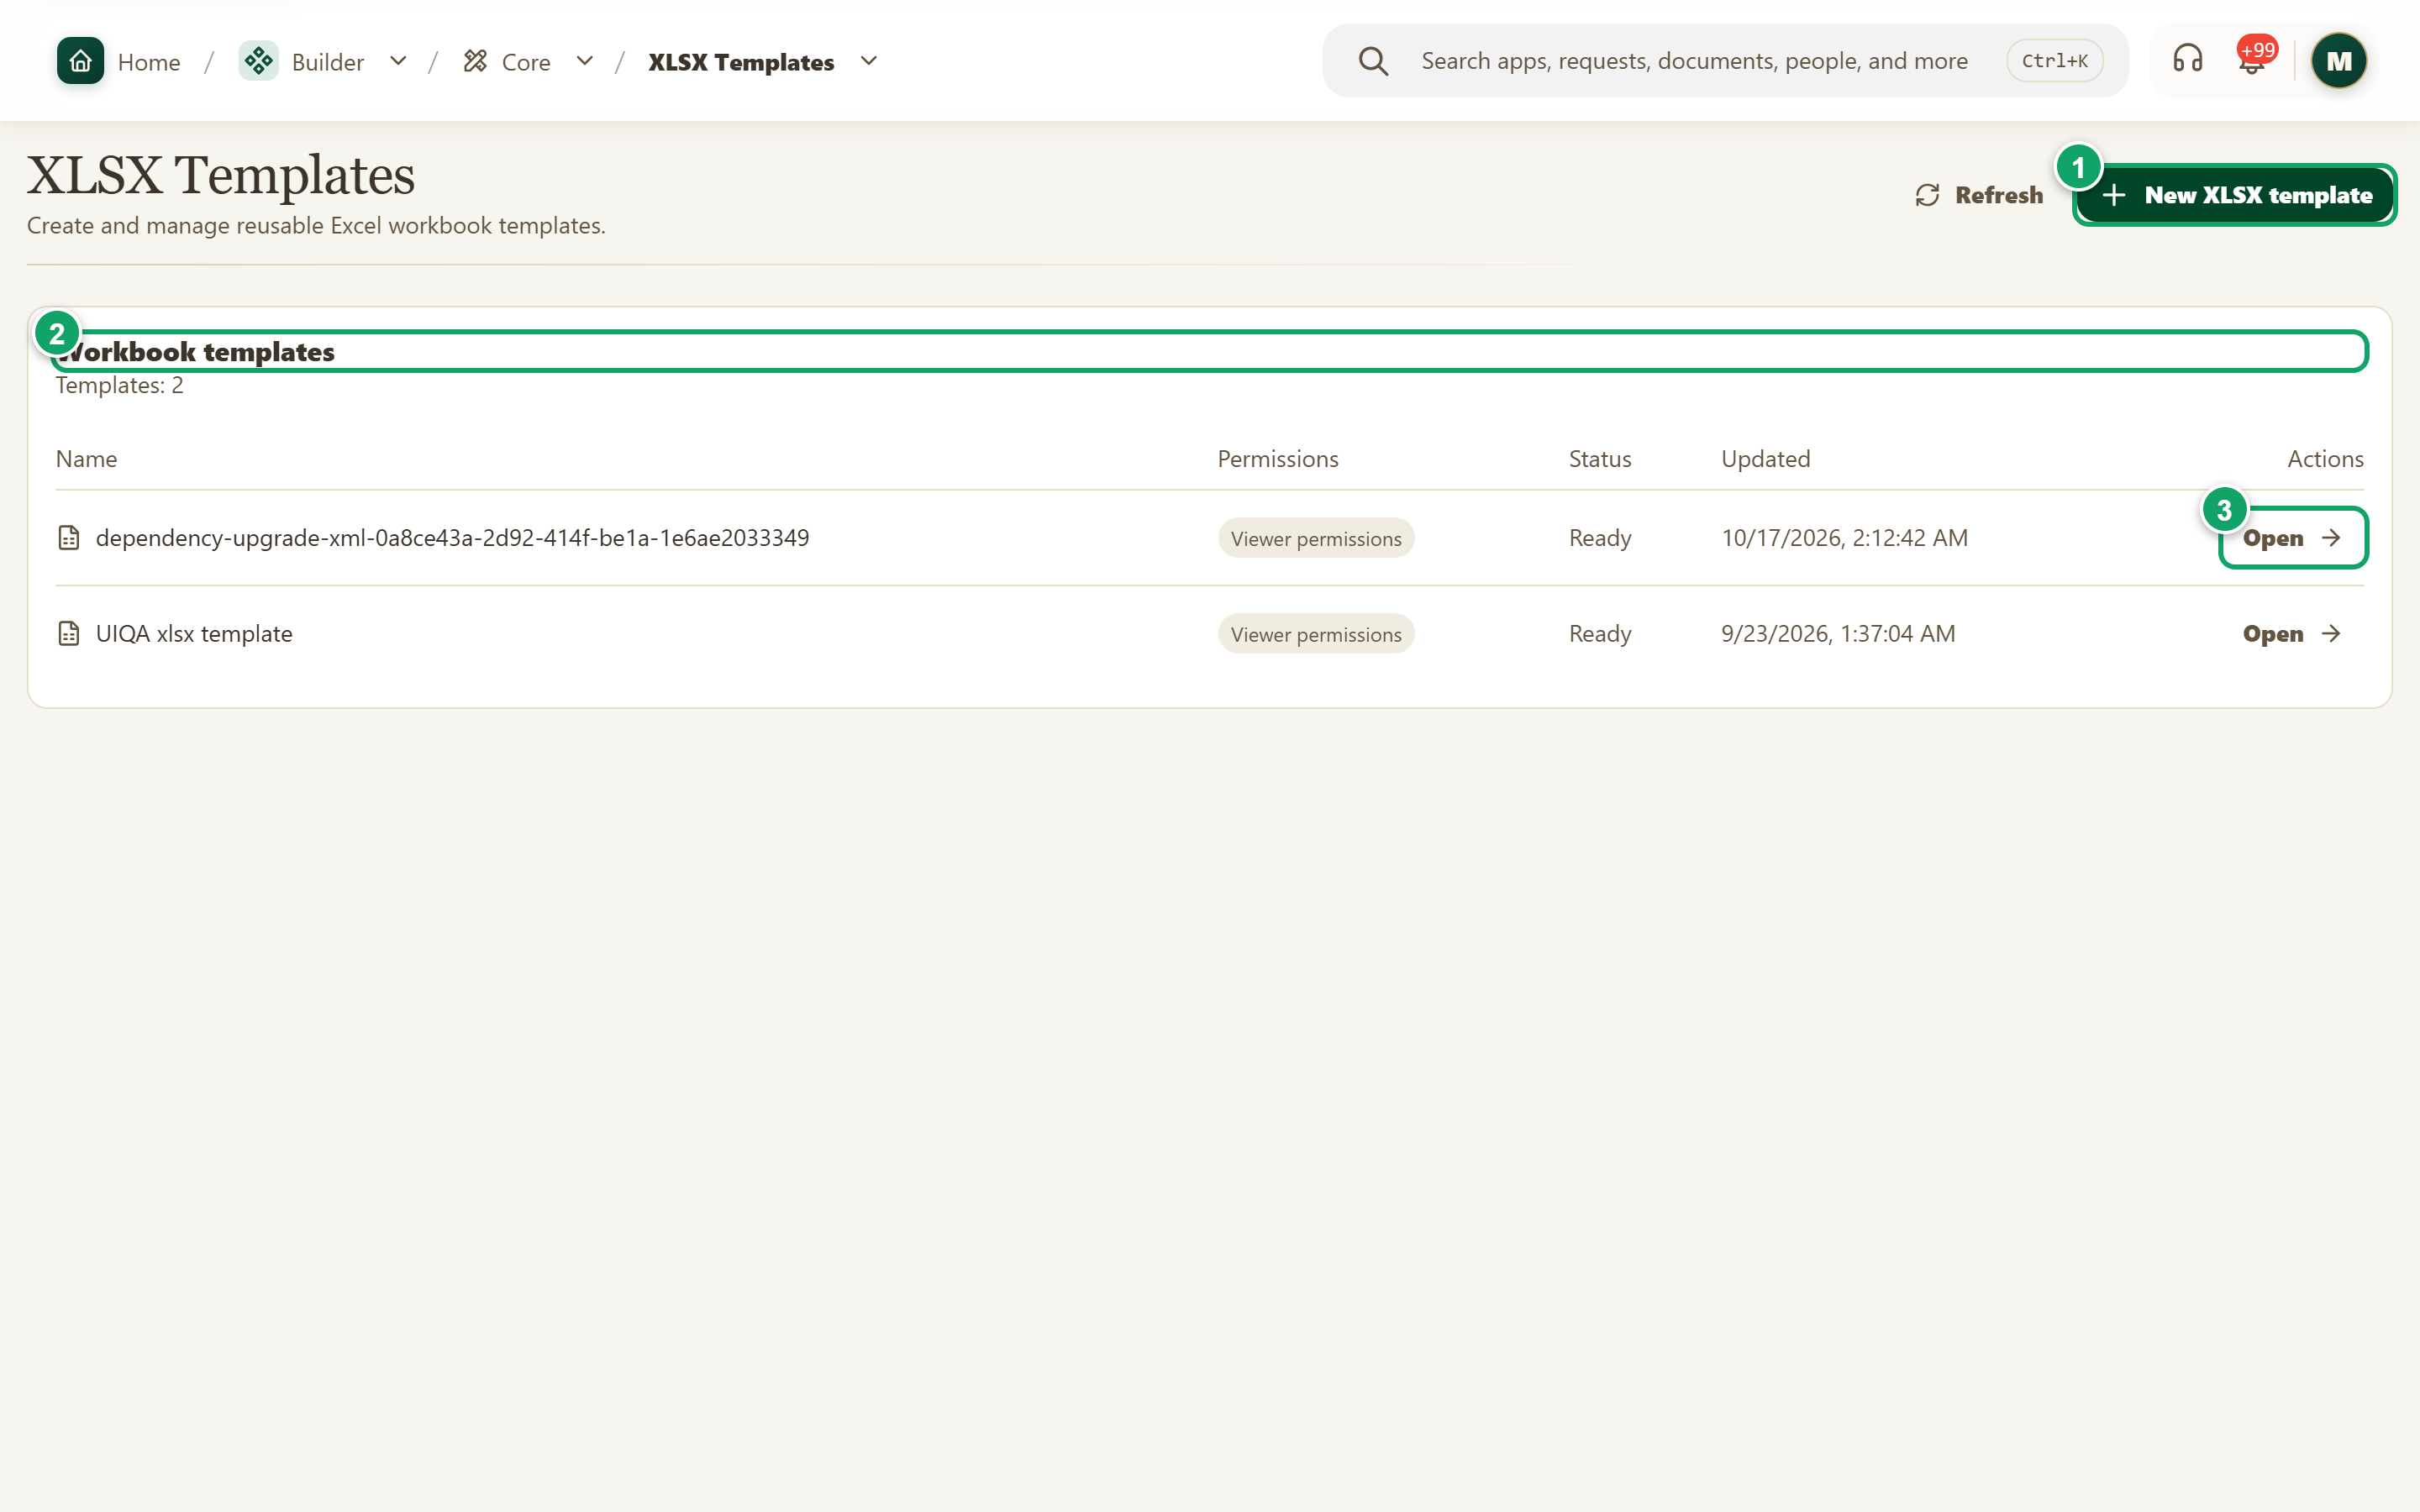
\includegraphics[width=0.95\linewidth,height=0.72\textheight,keepaspectratio]{figures/screens/ch06-xlsx-en.png}
\caption{The “XLSX Templates” page}
\label{fig:builder-xlsx-templates-screen}
\shotnote{The page lists workbook templates and their status, here test templates. ① “New XLSX template”: uploads an Excel workbook. ② “Workbook templates”: the list with status. ③ “Open”: opens a template to test it.}
\end{figure}


\begin{table}[H]
\centering
\caption{What do you find here?}
\label{tab:builder-xlsx-data}
\begin{tabularx}{\linewidth}{R{3.6cm} Y}
\rcHeaderRow
\thh{Part} & \thh{Content and action}\\
Workbook templates & The list of templates and their status: “Ready” or “Needs an Excel workbook”.\\
New XLSX template & Upload an “Excel workbook” and write the “Template name”; you can set the “Downloaded filename expression” and “Data permissions”.\\
Versions & Replace the workbook with a new version and review earlier versions.\\
Test \& download & Try the template with data, then “Render XLSX” or “Render PDF”.\\
Excel-specific tags & Repeat rows with \en{\{\{\#each\}\}}, repeat columns with \en{\{\{\#eachCol\}\}}, and hide a row or column when needed.\\
\end{tabularx}
\end{table}

\begin{figure}[H]
\centering
\begin{tikzpicture}[node distance=0.5cm]
\node[entity] (tpl) {XLSX template};
\node[entityOpt,below right=0.7cm and 0.3cm of tpl] (xlsx) {Excel file};
\node[entityOpt,below left=0.7cm and 0.3cm of tpl] (pdf) {PDF file};
\draw[dependsOnOpt] (tpl.south) -- ++(0,-0.3) -| (xlsx.north);
\draw[dependsOnOpt] (tpl.south) -- ++(0,-0.3) -| (pdf.north);
\end{tikzpicture}
\rclegend
\caption{The two output formats}
\label{fig:builder-xlsx-outputs}
\shotnote{The figure shows that one template produces an Excel or PDF file, and you choose what is allowed when linking it to the action with “Allow PDF”. Use Excel when the recipient needs to work with the numbers, and PDF when you want a fixed copy to view or archive.}
\end{figure}

\subsection{Steps and check}
\begin{enumerate}
\item Prepare the workbook in Excel and place the tags in the right cells.
\item Open “XLSX Templates” and press “New XLSX template”, upload the workbook, write the name and press “Create template”.
\item Try the template from “Test \& download”, then add a “Spreadsheet” action in the record type and link it to the template.
\end{enumerate}

\textbf{Check and recovery:} the template's status should be “Ready”, and the row should repeat for each item in the output file. If a number shows as text, put the tag alone in its cell. If you cannot create the template, managing templates needs Builder administration, not only a full seat.

\clearpage
\section{Print templates}
\label{sec:builder-feature-print-templates}

A print template is a document you design inside KayanOS by drag and drop, without uploading a Word file. It prints a form's requests or a record type's records as PDF or Word, on the organization's letterhead and identity. The “Print templates” page lists every existing template and its status; you create a new one from inside the form or record-type builder by pressing “Print”.

\textbf{Path and who uses it:} “Builder” → “Core” → “Print templates”. Used by those who build forms and record types.

\begin{rcnote}[Example: Horizon]
The system administrator opens the “Visit requests” type, presses “Print” and chooses “Start from this record type” to design a visit sheet with a verification QR code, then publishes it so it appears under “Print” on every request. They reach the template from ③.
\end{rcnote}

\begin{figure}[H]
\centering
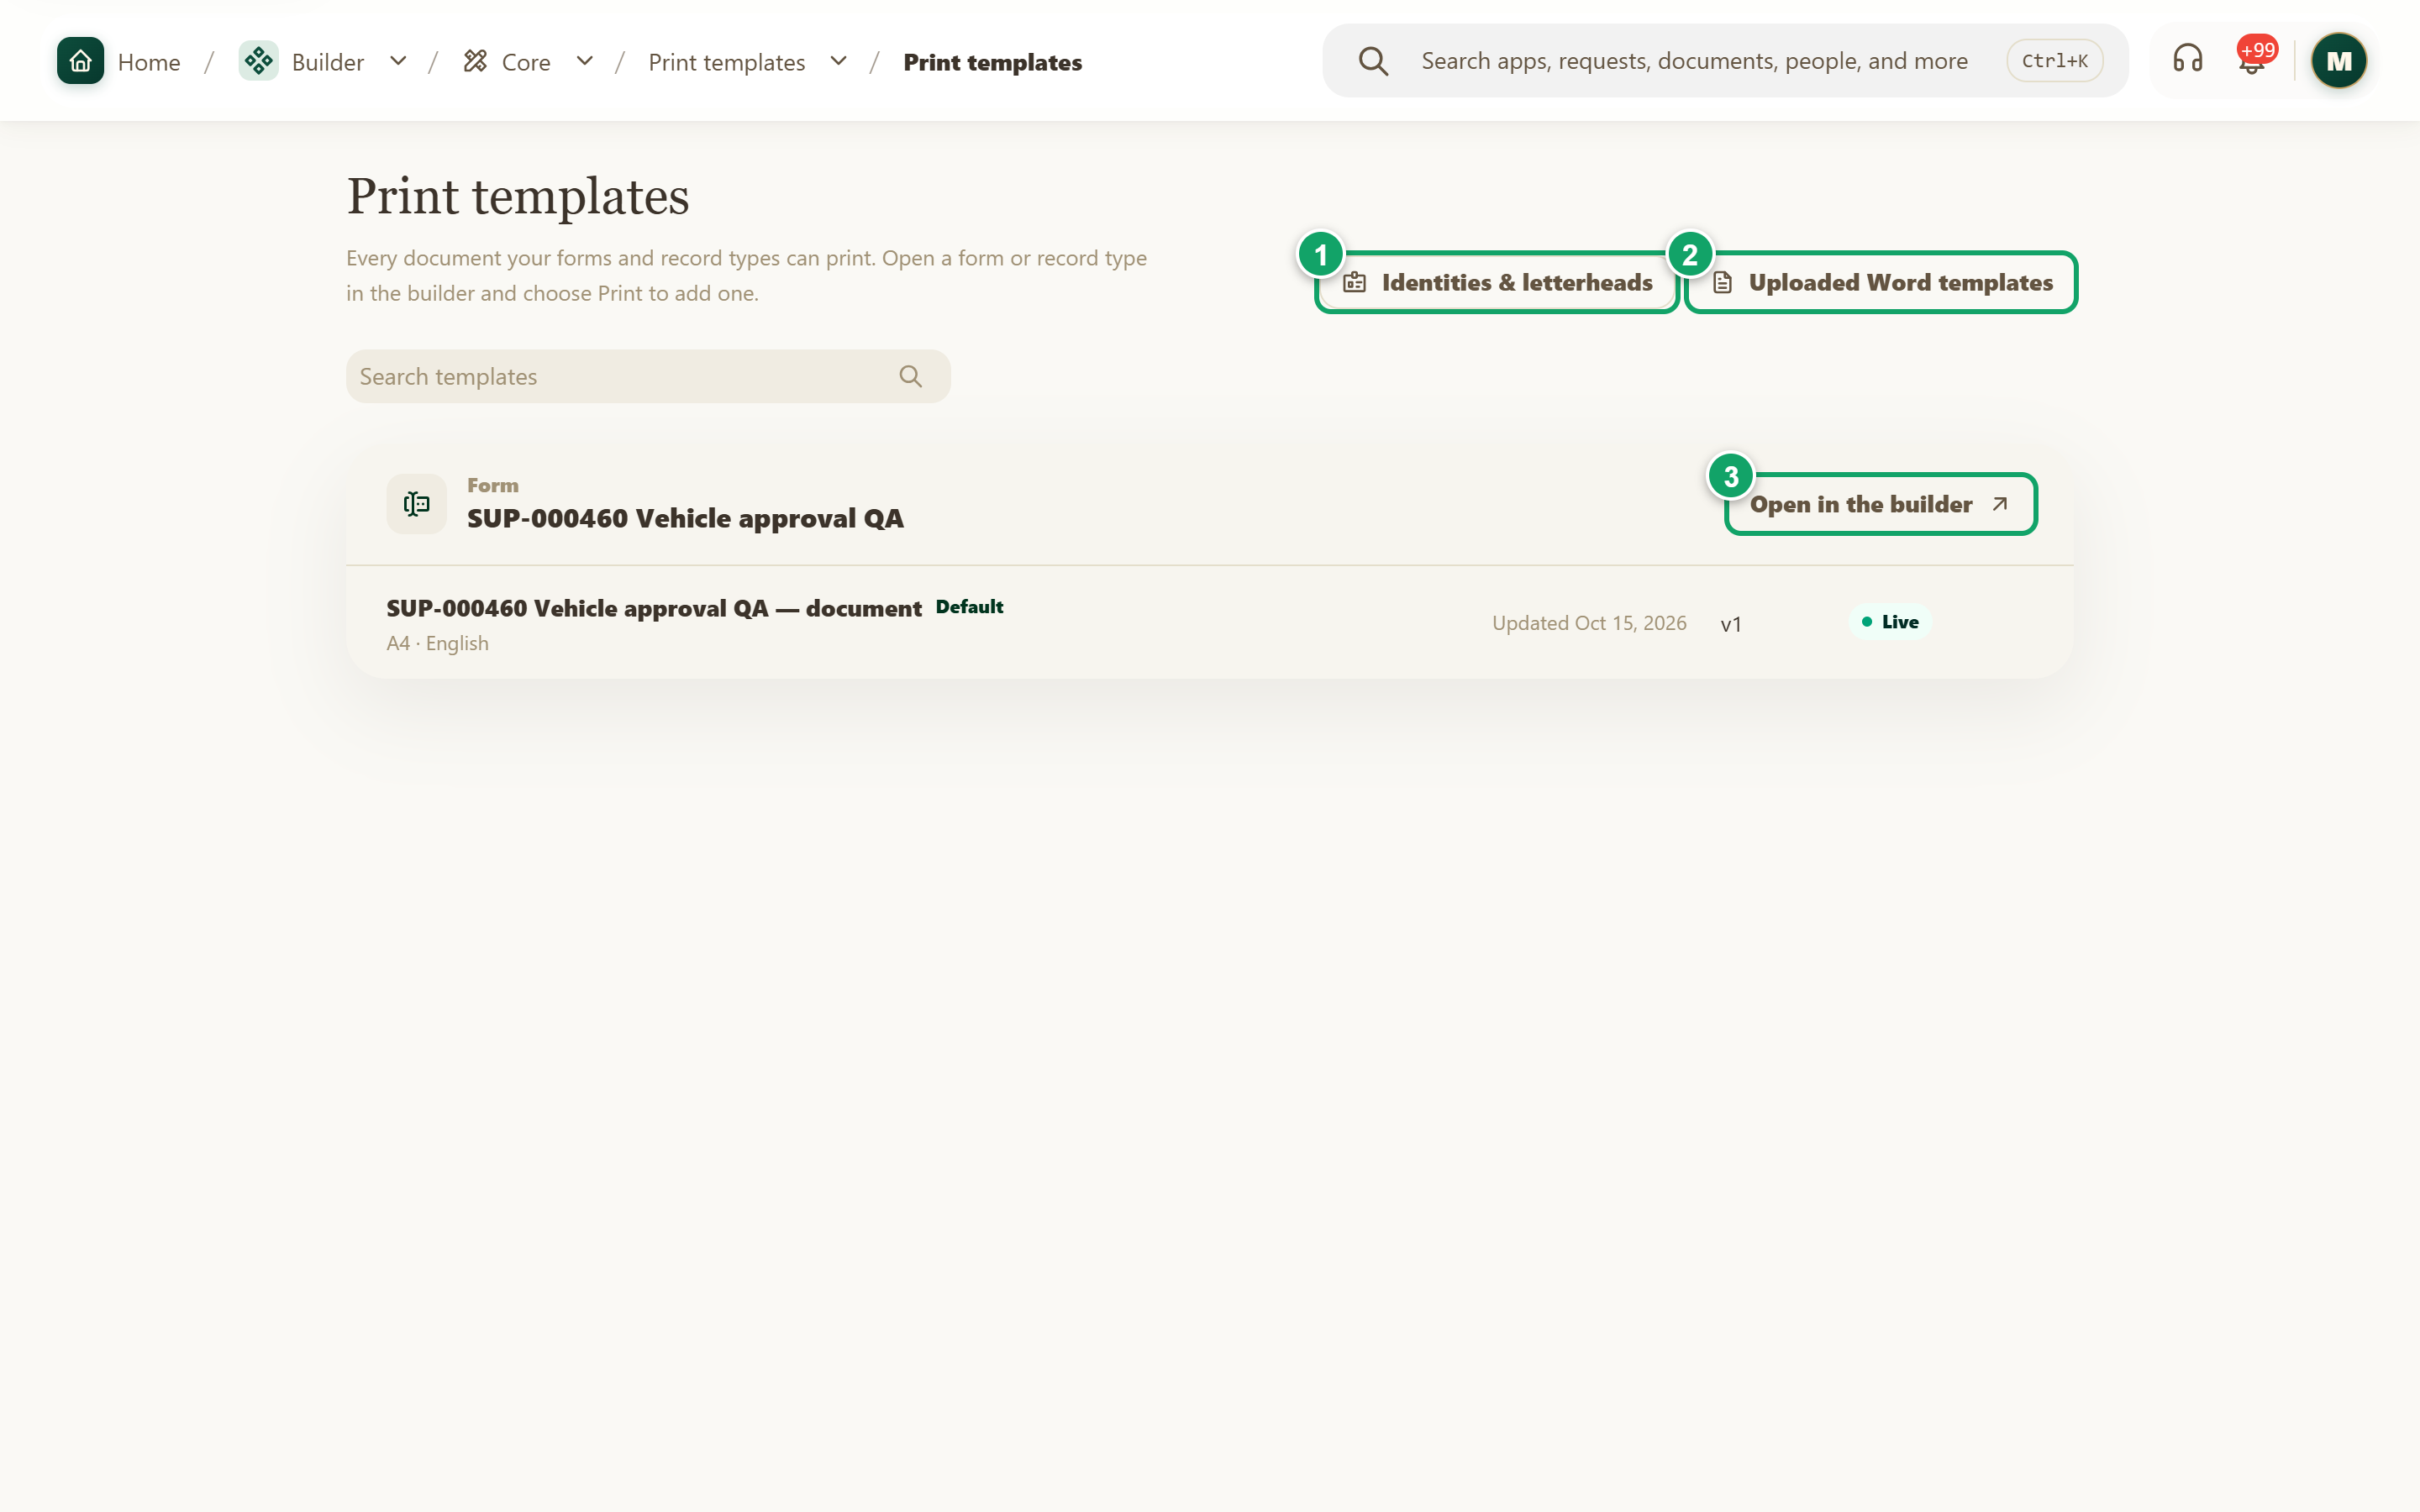
\includegraphics[width=0.95\linewidth,height=0.72\textheight,keepaspectratio]{figures/screens/ch06-print-en.png}
\caption{The “Print templates” library}
\label{fig:builder-print-templates-screen}
\shotnote{The page lists print templates grouped by form or record type, with their status. The template shown is a test template. ① “Identities \& letterheads”: goes to logos and letterheads. ② “Uploaded Word templates”: goes to DOCX templates. ③ “Open in the builder”: opens the form or type where the template is edited.}
\end{figure}


\begin{table}[H]
\centering
\caption{What do you find here?}
\label{tab:builder-print-data}
\begin{tabularx}{\linewidth}{R{3.6cm} Y}
\rcHeaderRow
\thh{Part} & \thh{Content and action}\\
Template library & Templates grouped by form or record type, with paper size, language, version and status: “Live”, “Draft” or “Unpublished changes”, plus “Open in the builder”.\\
New template & From the “Print” sheet in the builder: “Start from this form”, “Start from this record type” or “Blank page on the org letterhead”.\\
Editor & The “Data” tab for fields, “Blocks” such as text, table, image, logo, QR code, signature and approval trail, and “Page” for paper, margins, identity and letterhead.\\
Output & Formats people can download, the file name, “Who can print”, keeping a copy on the record, and a verification page opened by the QR code.\\
\end{tabularx}
\end{table}

\begin{figure}[H]
\centering
\begin{tikzpicture}[node distance=0.5cm]
\node[stepBox] (a) {Print from the form or type builder};
\node[stepBox,below=of a] (b) {Design data and blocks};
\node[stepBox,below=of b] (c) {Preview with a record};
\node[stepBox,below=of c] (d) {Publish};
\node[stepBox,below=of d] (e) {Print button on the record};
\draw[flowsTo] (a) -- (b);
\draw[flowsTo] (b) -- (c);
\draw[flowsTo] (c) -- (d);
\draw[flowsTo] (d) -- (e);
\end{tikzpicture}
\rclegend
\caption{From design to the print button}
\label{fig:builder-print-flow}
\shotnote{The diagram shows that a template is born inside the form or record-type builder, not on the library page, and is not offered to users before it is published. Previewing with a real record comes before publishing to catch empty fields or long tables before anyone prints them.}
\end{figure}

\subsection{Steps and check}
\begin{enumerate}
\item Open the form or record type in the builder, press “Print”, then choose a starting point.
\item Add fields and blocks, and set the paper, identity and letterhead under “Page”.
\item Press “Preview with a record” and “Download test PDF”, then set “Who can print” and press “Publish”.
\end{enumerate}

\textbf{Check and recovery:} the template should show as “Live” in the library and appear in “Choose a document” when pressing “Print” on a record. If it does not, make sure it is published, because a template is “Not offered until published”; use “Check against all records” to find records missing data.

\clearpage
\section{Identities \& letterheads}
\label{sec:builder-feature-identities}

An identity is the organization's logo, name, colours and official details, such as its registration number and address. A letterhead is the page header and footer shown in printed documents. This page keeps both in one place, so print templates and official correspondence share them, and any change here shows in all of them at the next print.

\textbf{Path and who uses it:} “Builder” → “Core” → “Identities \& letterheads”. Used by those who manage how the organization's documents look.

\begin{rcnote}[Example: Horizon]
The system administrator uploads Horizon's logo and adds its official details to the default identity, then creates a letterhead whose header shows on the first page only, so the visit sheet prints with the company logo without redesigning it in every template. They upload the logo in ③ and save from ④, then create the letterhead from ②.
\end{rcnote}

\begin{figure}[H]
\centering
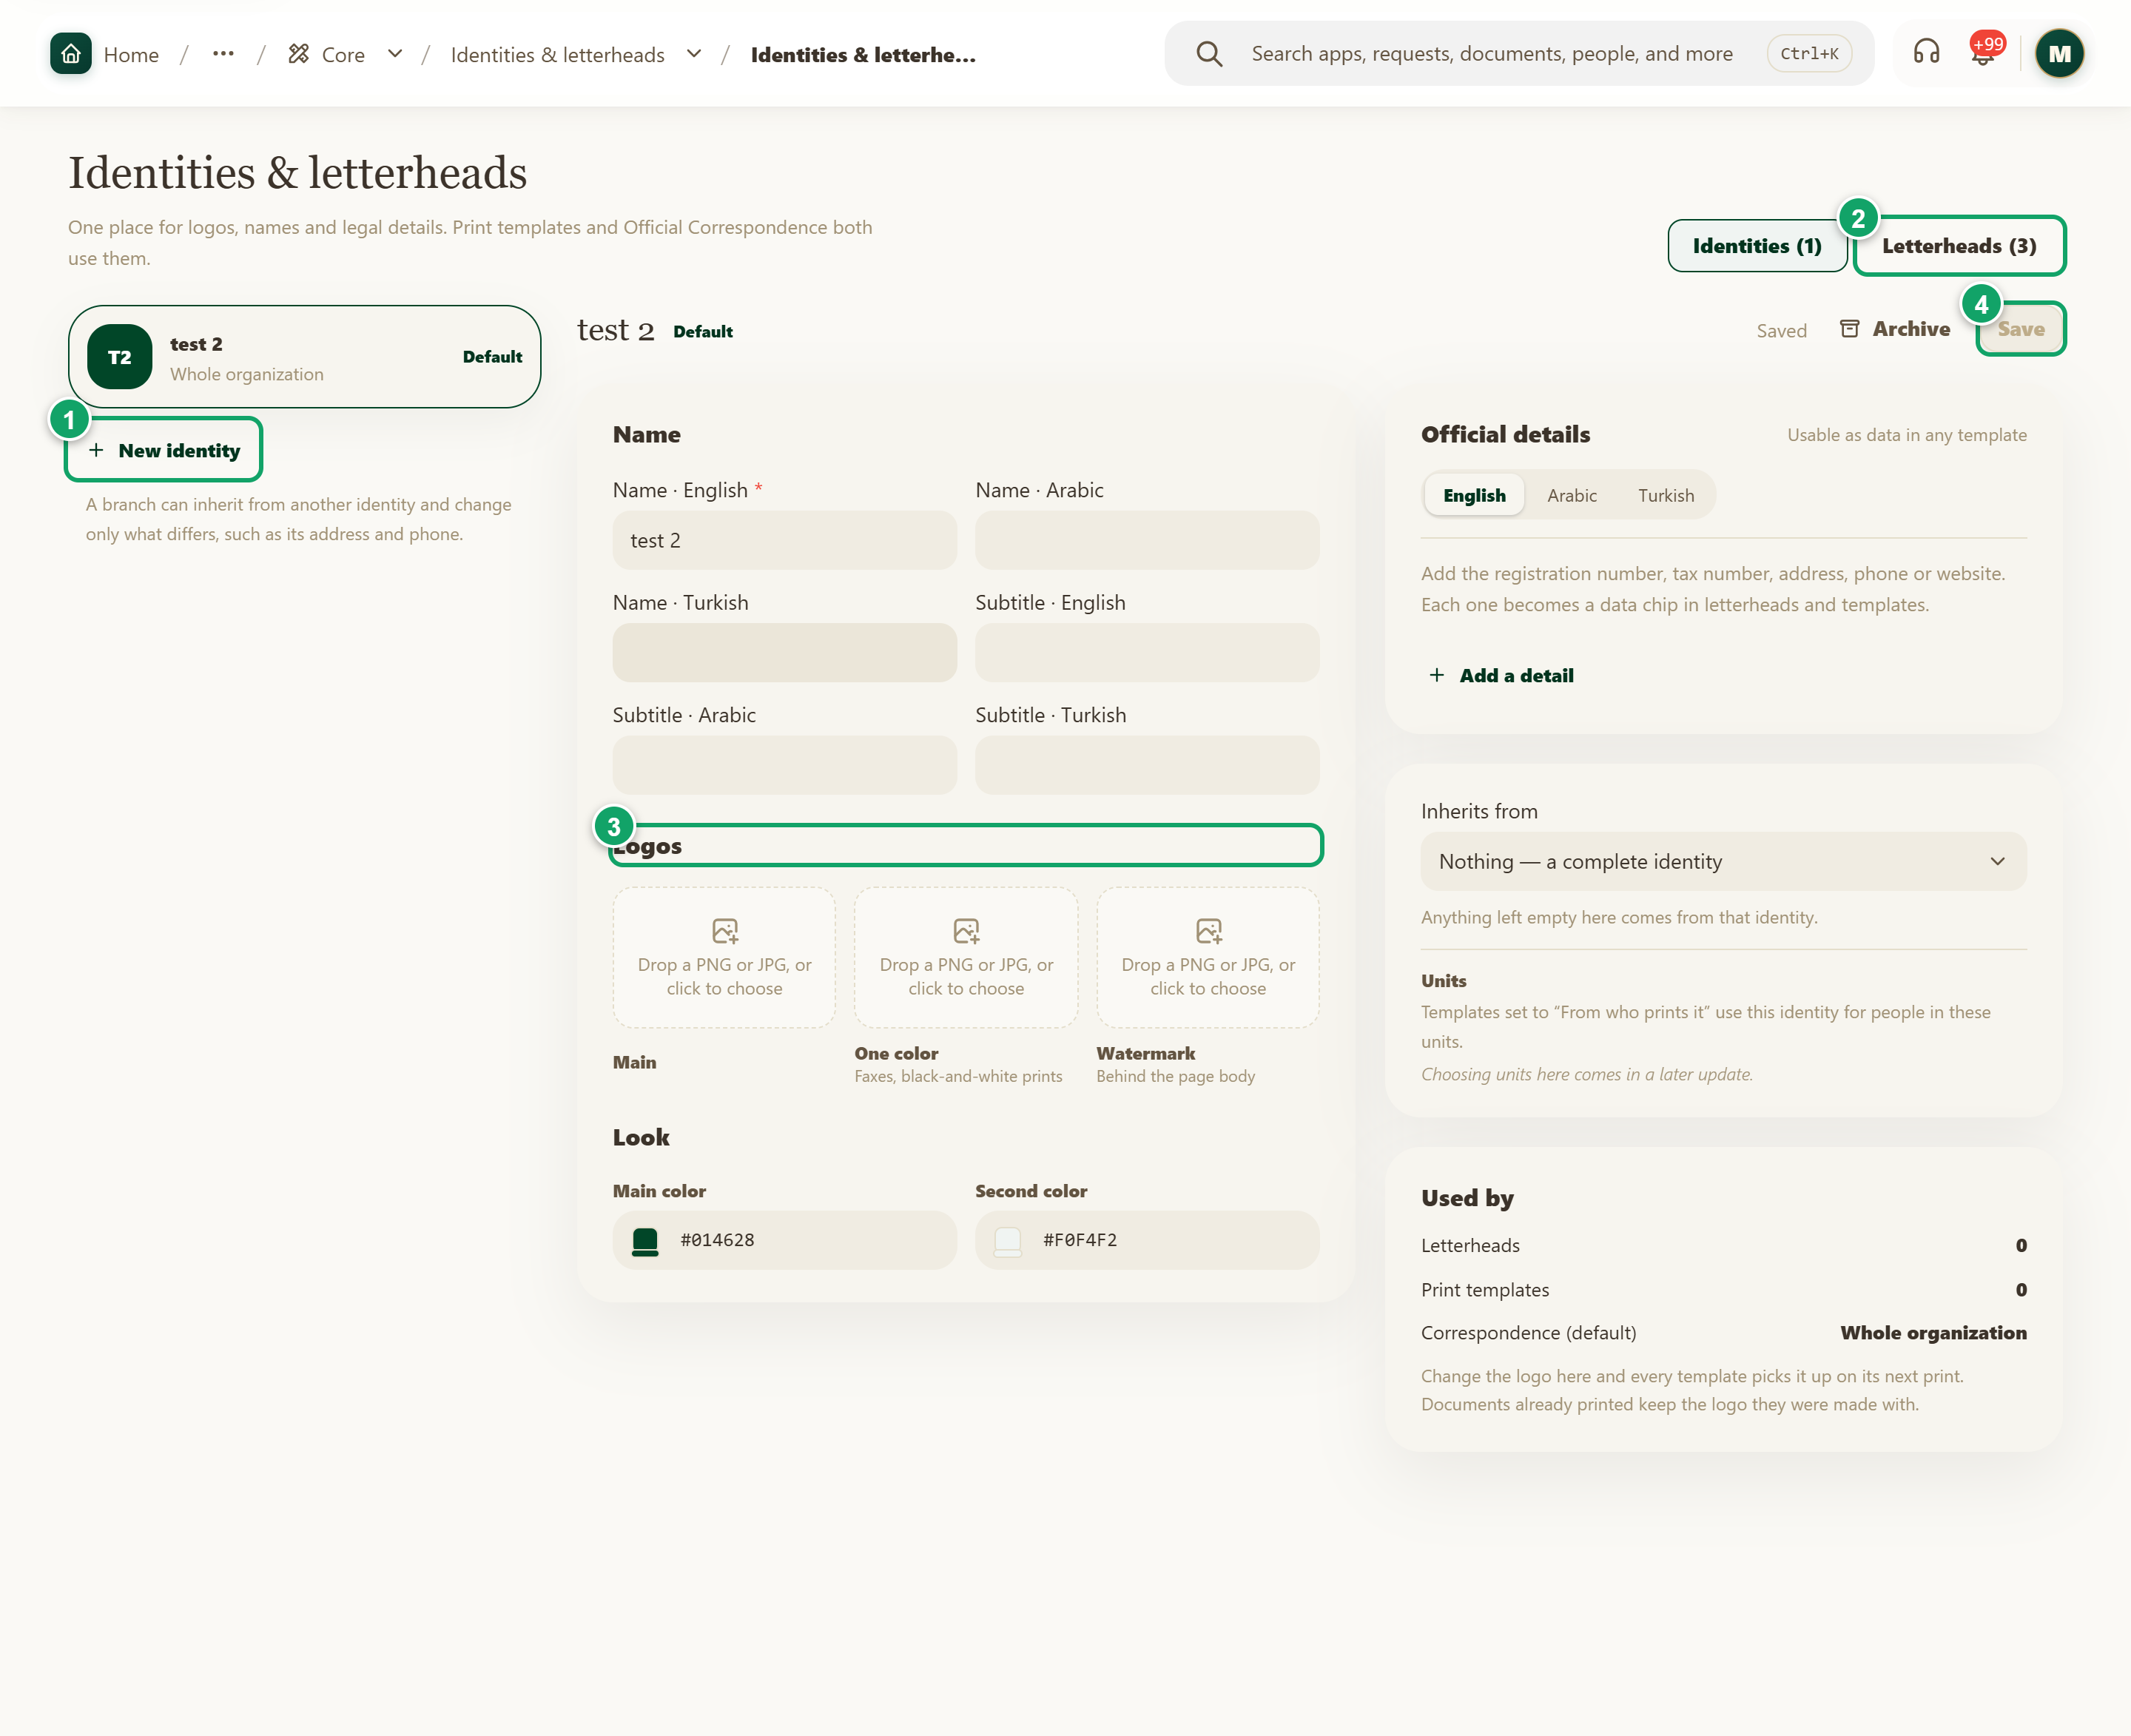
\includegraphics[width=0.95\linewidth,height=0.72\textheight,keepaspectratio]{figures/screens/ch06-identities-en.png}
\caption{The “Identities \& letterheads” page}
\label{fig:builder-identities-screen}
\shotnote{The page shows the organization’s default identity and its fields, here the test organization’s identity. ① “New identity”: creates another identity, such as a branch identity. ② “Letterheads”: the shared letterheads tab. ③ “Logos”: main, one-color and watermark logos. ④ “Save”: saves identity changes.}
\end{figure}


\begin{table}[H]
\centering
\caption{What do you find here?}
\label{tab:builder-identities-data}
\begin{tabularx}{\linewidth}{R{3.6cm} Y}
\rcHeaderRow
\thh{Part} & \thh{Content and action}\\
Identities & Each identity has a “Name” and “Subtitle” in every language, “Logos” (main, one color, watermark), a “Look” with two colours, and “Official details”.\\
Inherits from & Lets an identity take what it does not set from another identity, such as a branch identity inheriting from the organization's.\\
Used by & Shows the letterheads, print templates and correspondence that rely on the identity.\\
Letterheads & Each letterhead has a name and language, items such as the logo, print date, QR code and page number, and whether the header and footer show on every page or the first only.\\
\end{tabularx}
\end{table}

\begin{figure}[H]
\centering
\begin{tikzpicture}[node distance=0.5cm]
\node[entity] (id) {Identity};
\node[entityOpt,below=0.7cm of id] (lh) {Letterhead};
\node[entityOpt,below right=0.7cm and 0.3cm of lh] (print) {Print templates};
\node[entityOpt,below left=0.7cm and 0.3cm of lh] (corr) {Official correspondence};
\draw[dependsOnOpt] (id) -- (lh);
\draw[dependsOnOpt] (lh.south) -- ++(0,-0.3) -| (print.north);
\draw[dependsOnOpt] (lh.south) -- ++(0,-0.3) -| (corr.north);
\end{tikzpicture}
\rclegend
\caption{From identity to the printed document}
\label{fig:builder-identities-model}
\shotnote{The figure shows that the identity feeds the letterhead, and the letterhead is shared by print templates and official correspondence. So change the logo or official details in the identity once, and the change shows in every document printed afterwards; review “Used by” before any change.}
\end{figure}

\subsection{Steps and check}
\begin{enumerate}
\item Open “Identities \& letterheads”, choose the default “Whole organization” identity or create a “New identity”.
\item Write the name in each language, upload the logos as PNG or JPG, add the official details, then press “Save”.
\item Open “Letterheads”, create a “New letterhead”, and choose its items and where they show.
\end{enumerate}

\textbf{Check and recovery:} print a test document from a template using the letterhead; the logo and new details should appear. If you cannot archive an identity, make another identity the default first, because the default identity cannot be archived.

\clearpage
\section{Dashboards}
\label{sec:builder-feature-dashboards}

A dashboard is a page of numbers and charts that summarizes the work, such as the number of open requests or the average time to finish. You build it from widgets that take their data from a record type, form submissions or other sources, then publish it and place it in navigation. Each viewer sees the data their permissions allow, so a dashboard never goes around anyone's access.

\textbf{Path and who uses it:} “Builder” → “Core” → “Dashboards”. Built by those allowed to create dashboards, and viewed by those given access.

\begin{rcnote}[Example: Horizon]
Horizon builds a “Visit tracking” dashboard with a figure for pending requests, a chart of visits by branch and a calendar of their dates, which Sarah Al-Khatib reviews every week. The dashboard starts from ①.
\end{rcnote}

\begin{figure}[H]
\centering
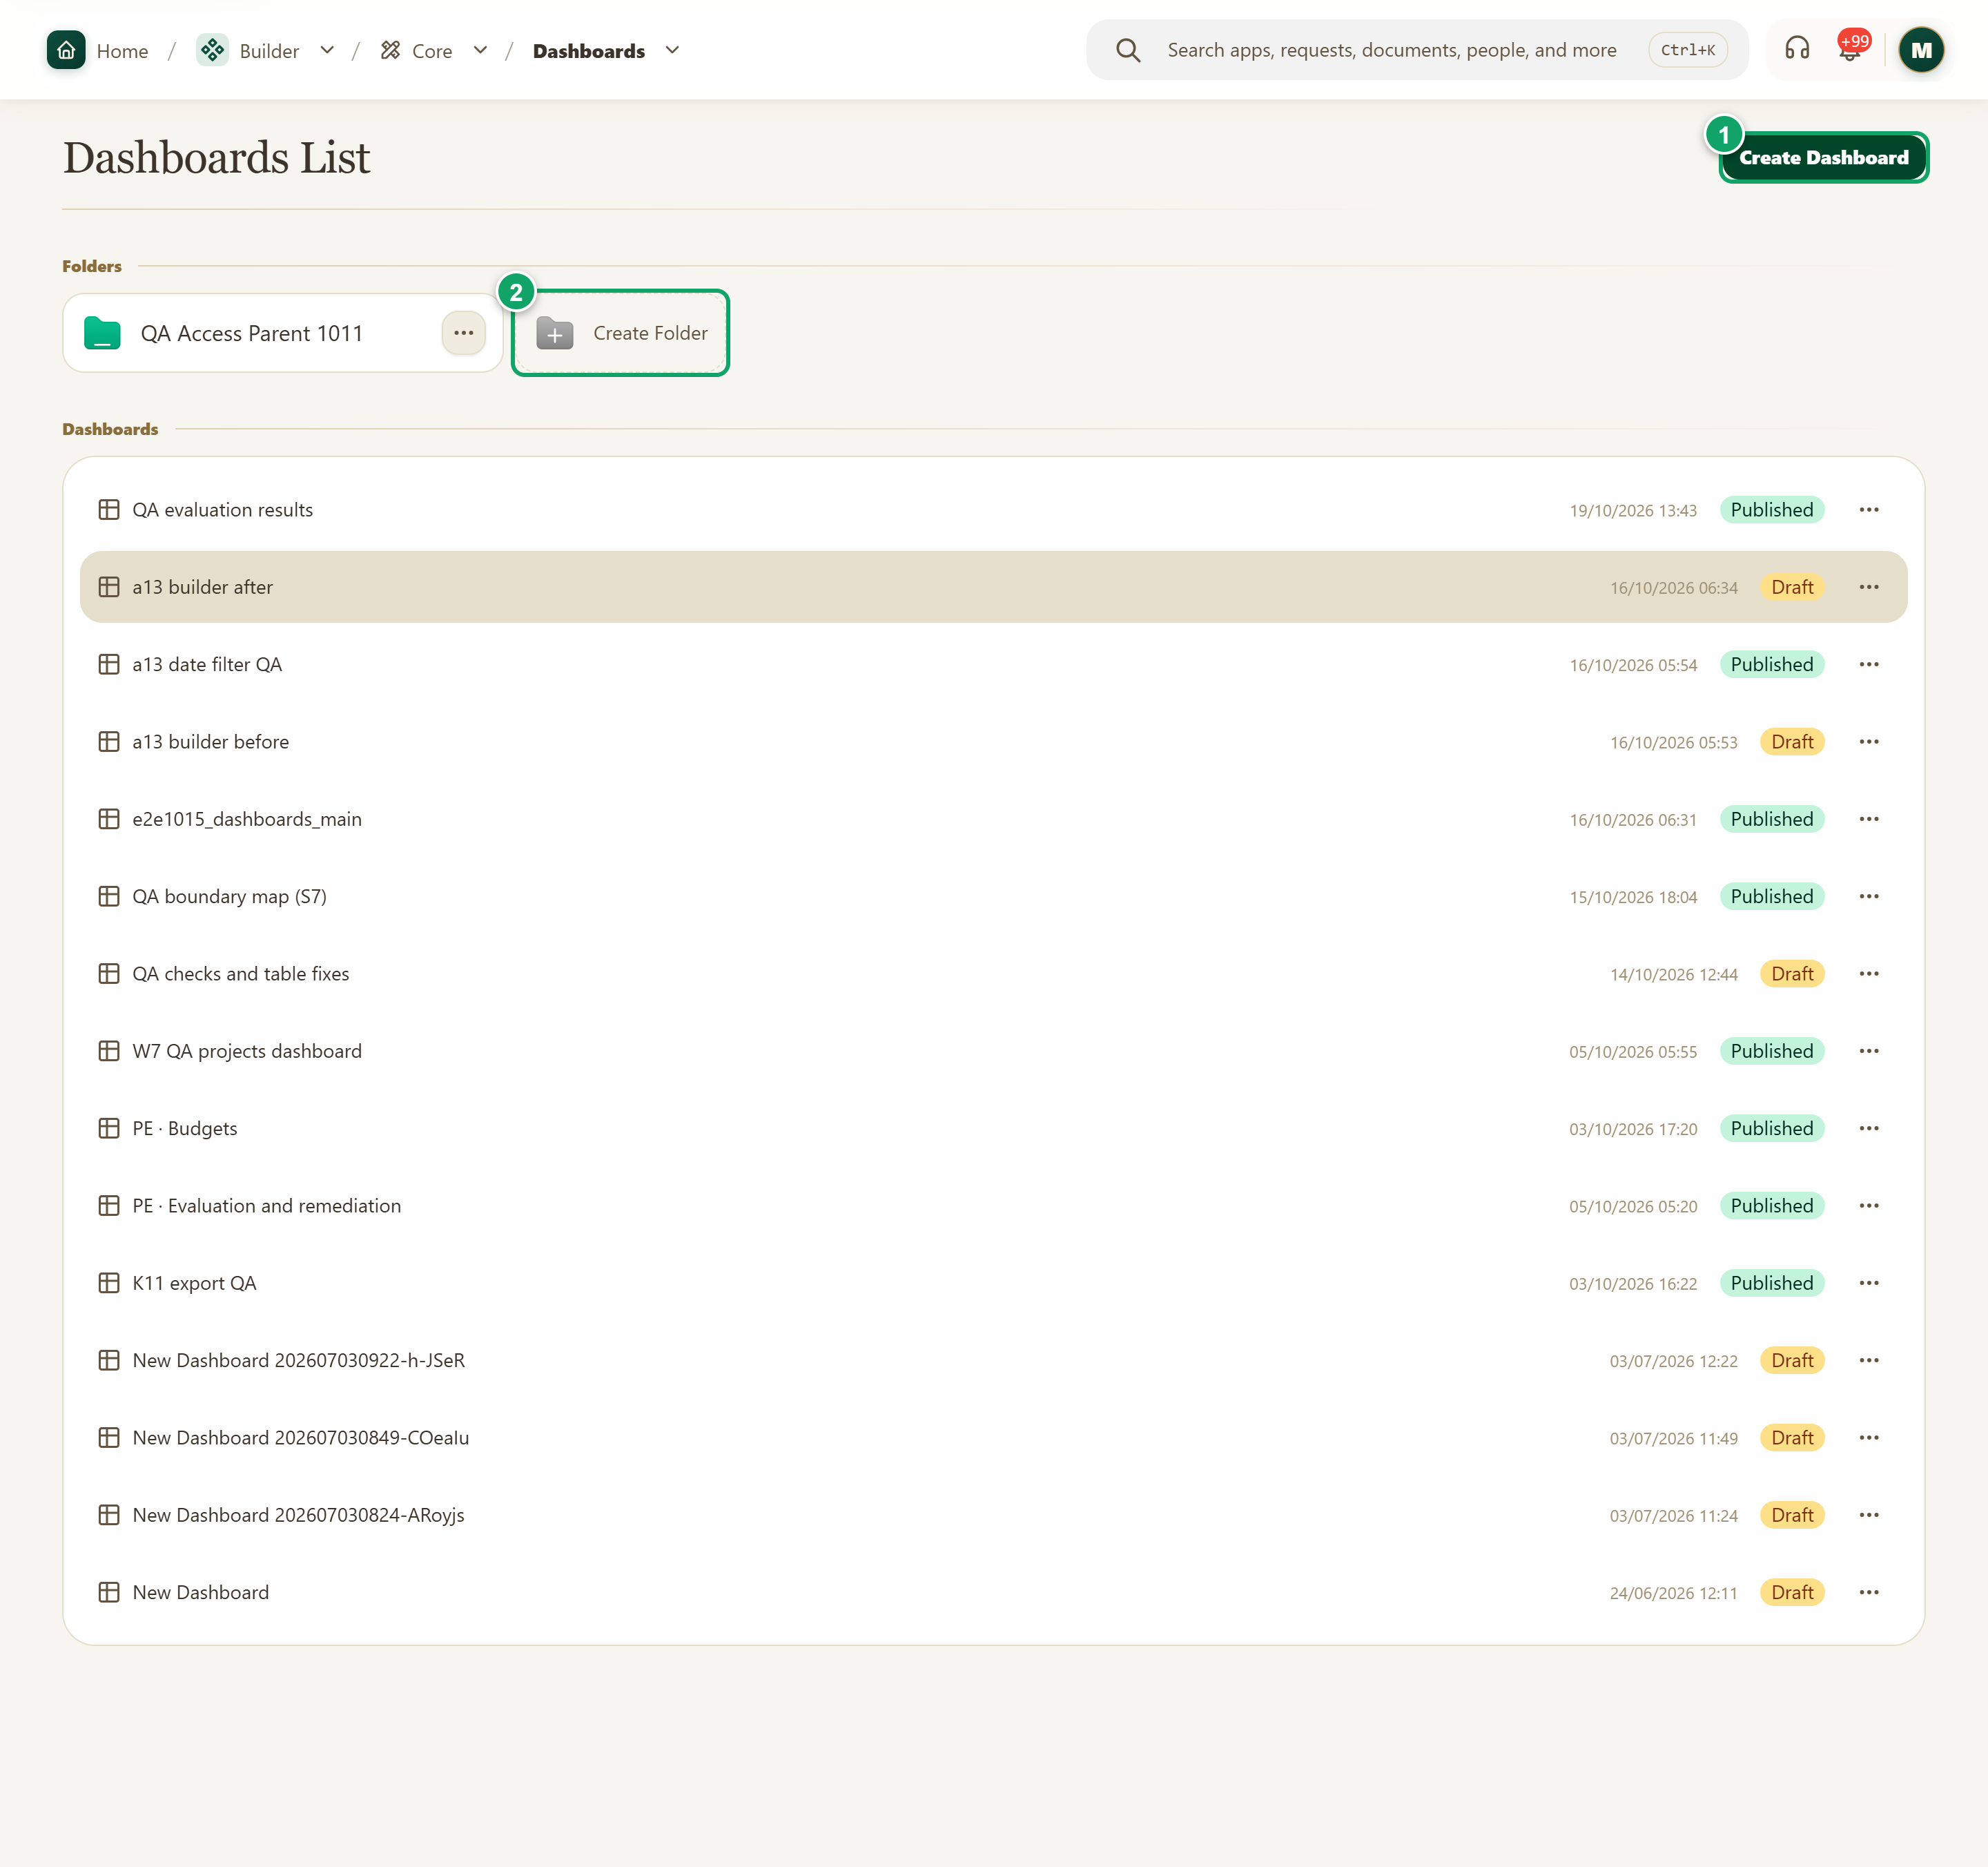
\includegraphics[width=0.95\linewidth,height=0.72\textheight,keepaspectratio]{figures/screens/ch06-dashboards-en.png}
\caption{The “Dashboards” page}
\label{fig:builder-dashboards-screen}
\shotnote{The page shows folders and dashboards with their status, here test dashboards. ① “Create Dashboard”: starts a new dashboard. ② “Create Folder”: organizes dashboards in folders.}
\end{figure}


\begin{table}[H]
\centering
\caption{What do you find here?}
\label{tab:builder-dashboards-data}
\begin{tabularx}{\linewidth}{R{3.6cm} Y}
\rcHeaderRow
\thh{Part} & \thh{Content and action}\\
Dashboards List & Dashboards and folders with their status, “Draft” or “Published”, and the buttons “Create Dashboard” and “Create Folder”.\\
Widgets & “Add Section”, then “Add Widget”: chart, figure, KPI, table, progress, calendar, map and more.\\
Data source & Entity, form submissions, SOP, manual data and others, with the data access level.\\
Filters & Let the viewer change the date range for the whole dashboard or for chosen sections or widgets.\\
Settings and access & Name, description, “Show in Navigation”, app and section, and “Manage access” to decide who views it.\\
Versions and publishing & “Publish” creates a new version that replaces the live one, and “Version history” lets you restore.\\
\end{tabularx}
\end{table}

\begin{figure}[H]
\centering
\begin{tikzpicture}[node distance=0.5cm]
\node[stepBox] (a) {Create Dashboard};
\node[stepBox,below=of a] (b) {Sections, widgets, sources};
\node[stepBox,below=of b] (c) {Preview and compare};
\node[stepBox,below=of c] (d) {Publish and show in navigation};
\draw[flowsTo] (a) -- (b);
\draw[flowsTo] (b) -- (c);
\draw[flowsTo] (c) -- (d);
\end{tikzpicture}
\rclegend
\caption{Building a dashboard}
\label{fig:builder-dashboards-flow}
\shotnote{The diagram puts the comparison with known records before publishing, because a wrong number on a dashboard leads to a wrong decision. If you know five requests are waiting for a decision, the widget must show five. The team does not see the dashboard in navigation before it is published.}
\end{figure}

\subsection{Steps and check}
\begin{enumerate}
\item Open “Dashboards” and press “Create Dashboard”, then write the name and a clear description.
\item Add a section, then a widget, choose its data source, fields and filters, and give it a title that says what it counts.
\item Press “Preview” and compare the numbers with records you know, then set where it appears in the settings and press “Publish”.
\end{enumerate}

\textbf{Check and recovery:} open the dashboard from navigation as a viewer; it should show the expected numbers. If the message “This dashboard isn't published yet” appears, publish it; if one user sees smaller numbers than another, it is because the dashboard shows what their permissions allow.

\clearpage
\section{Pages}
\label{sec:builder-feature-pages}

A page places a saved dashboard from the AI analytics workspace (\en{DB Genie}) inside an app section, so members see it as a menu item. It is the way to share a dashboard you made in “AI Dashboards” with the team.

\textbf{Path and who uses it:} “Builder” → “Core” → “Pages”. Available only to the organization owner and administrator.

\begin{rcnote}[Example: Horizon]
The system administrator makes an analysis of visit completion times in the AI workspace, then publishes it as a page in the “Visits” section of “Branch services” for Sarah Al-Khatib to see. The page starts from ①.
\end{rcnote}

\begin{figure}[H]
\centering
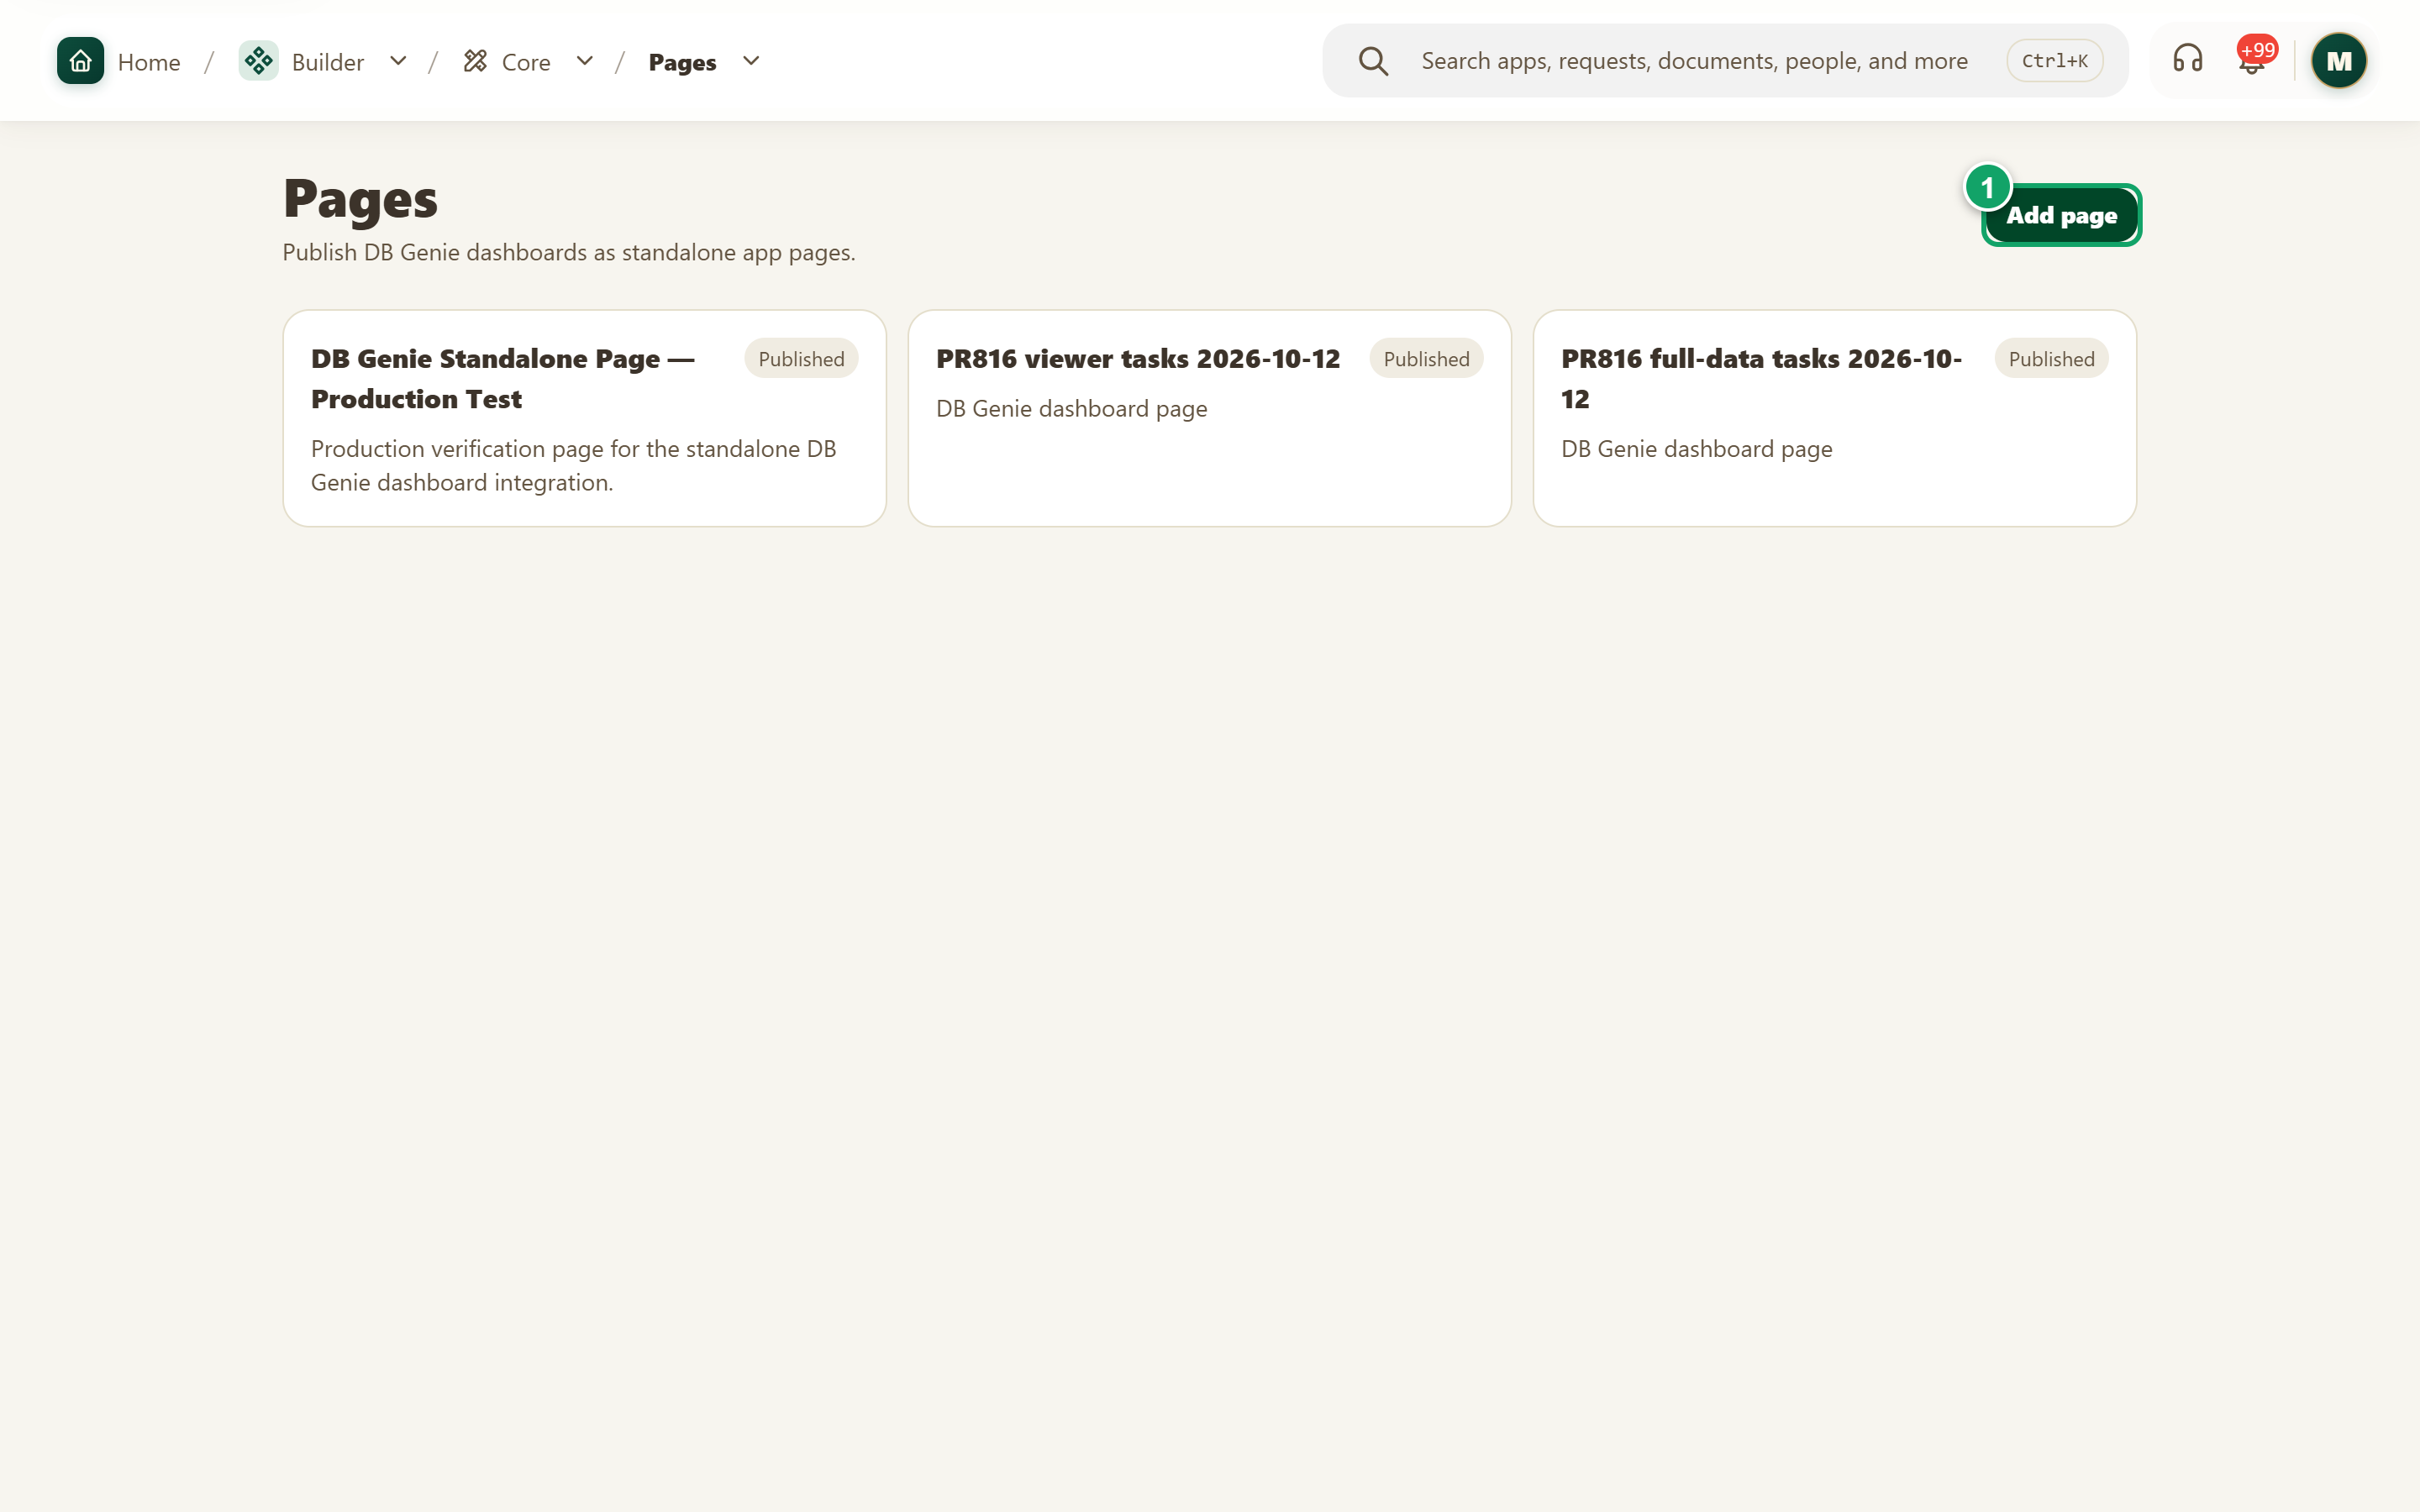
\includegraphics[width=0.95\linewidth,height=0.72\textheight,keepaspectratio]{figures/screens/ch06-pages-en.png}
\caption{The “Pages” page}
\label{fig:builder-pages-screen}
\shotnote{The page lists standalone pages published in apps, here test pages. ① “Add page”: starts a new page where you choose its dashboard, app and section.}
\end{figure}


\begin{table}[H]
\centering
\caption{The page's fields}
\label{tab:builder-pages-data}
\begin{tabularx}{\linewidth}{R{3.6cm} Y}
\rcHeaderRow
\thh{Field} & \thh{Meaning}\\
Title and Description & The page name as it appears in the menu, and a short description.\\
App and Section & Where the page appears in navigation.\\
DB Genie dashboard & A saved dashboard chosen with “Choose dashboard”.\\
Data shown & “With the viewer's permissions”, the safest choice, or organization data with guards, or all organization data without checking the viewer's scope.\\
Status & “Draft”, “Published” or “Archived”. The page appears in navigation only when published.\\
\end{tabularx}
\end{table}

\begin{figure}[H]
\centering
\begin{tikzpicture}[node distance=0.5cm]
\node[stepBox] (a) {Dashboard in the AI workspace};
\node[stepBox,below=of a] (b) {Add page, choose the dashboard};
\node[stepBox,below=of b] (c) {Status: Published};
\node[stepBox,below=of c] (d) {Grant roles the view right};
\draw[flowsTo] (a) -- (b);
\draw[flowsTo] (b) -- (c);
\draw[flowsTo] (c) -- (d);
\end{tikzpicture}
\rclegend
\caption{From a private dashboard to a team page}
\label{fig:builder-pages-flow}
\shotnote{The diagram shows that publishing the page is not enough for members to see it; each role also needs the right to view the page in the role settings. The original dashboard stays as it is, so deleting the page does not delete the dashboard.}
\end{figure}

\subsection{Steps and check}
\begin{enumerate}
\item Save the dashboard in “AI Dashboards” first.
\item Open “Pages” and press “Add page”, then write the title and choose the app, section and dashboard.
\item Choose “With the viewer's permissions” under “Data shown”, set the status to “Published”, then press “Save page”.
\item Give the right roles the right to view the page in the role settings.
\end{enumerate}

\textbf{Check and recovery:} the page should appear in the chosen section for those allowed to view it. If the message “Title, app, section, and dashboard are required.” appears, complete the four fields. If a member does not see it, check its status and their role's right.

\clearpage
\section{AI Dashboards}
\label{sec:builder-feature-ai-dashboards}

This page opens the AI analytics workspace (\en{DB Genie}), where you describe what you want to know and a dashboard is built for you from the organization's data. The workspace is private to you and uses only the data you can read. To share a dashboard with the team, publish it from the “Pages” page.

\textbf{Path and who uses it:} “Builder” → “Core” → “AI Dashboards”. Shown to those whose seat includes analytics, if they are an organization administrator or hold the right to view dashboards.

\begin{rcnote}[Example: Horizon]
Sarah Al-Khatib asks for a dashboard showing the number of visits per branch each month, and reviews the result in her private workspace before the system administrator decides to publish it as a team page. Sarah requests the dashboard inside workspace ①.
\end{rcnote}

\begin{figure}[H]
\centering
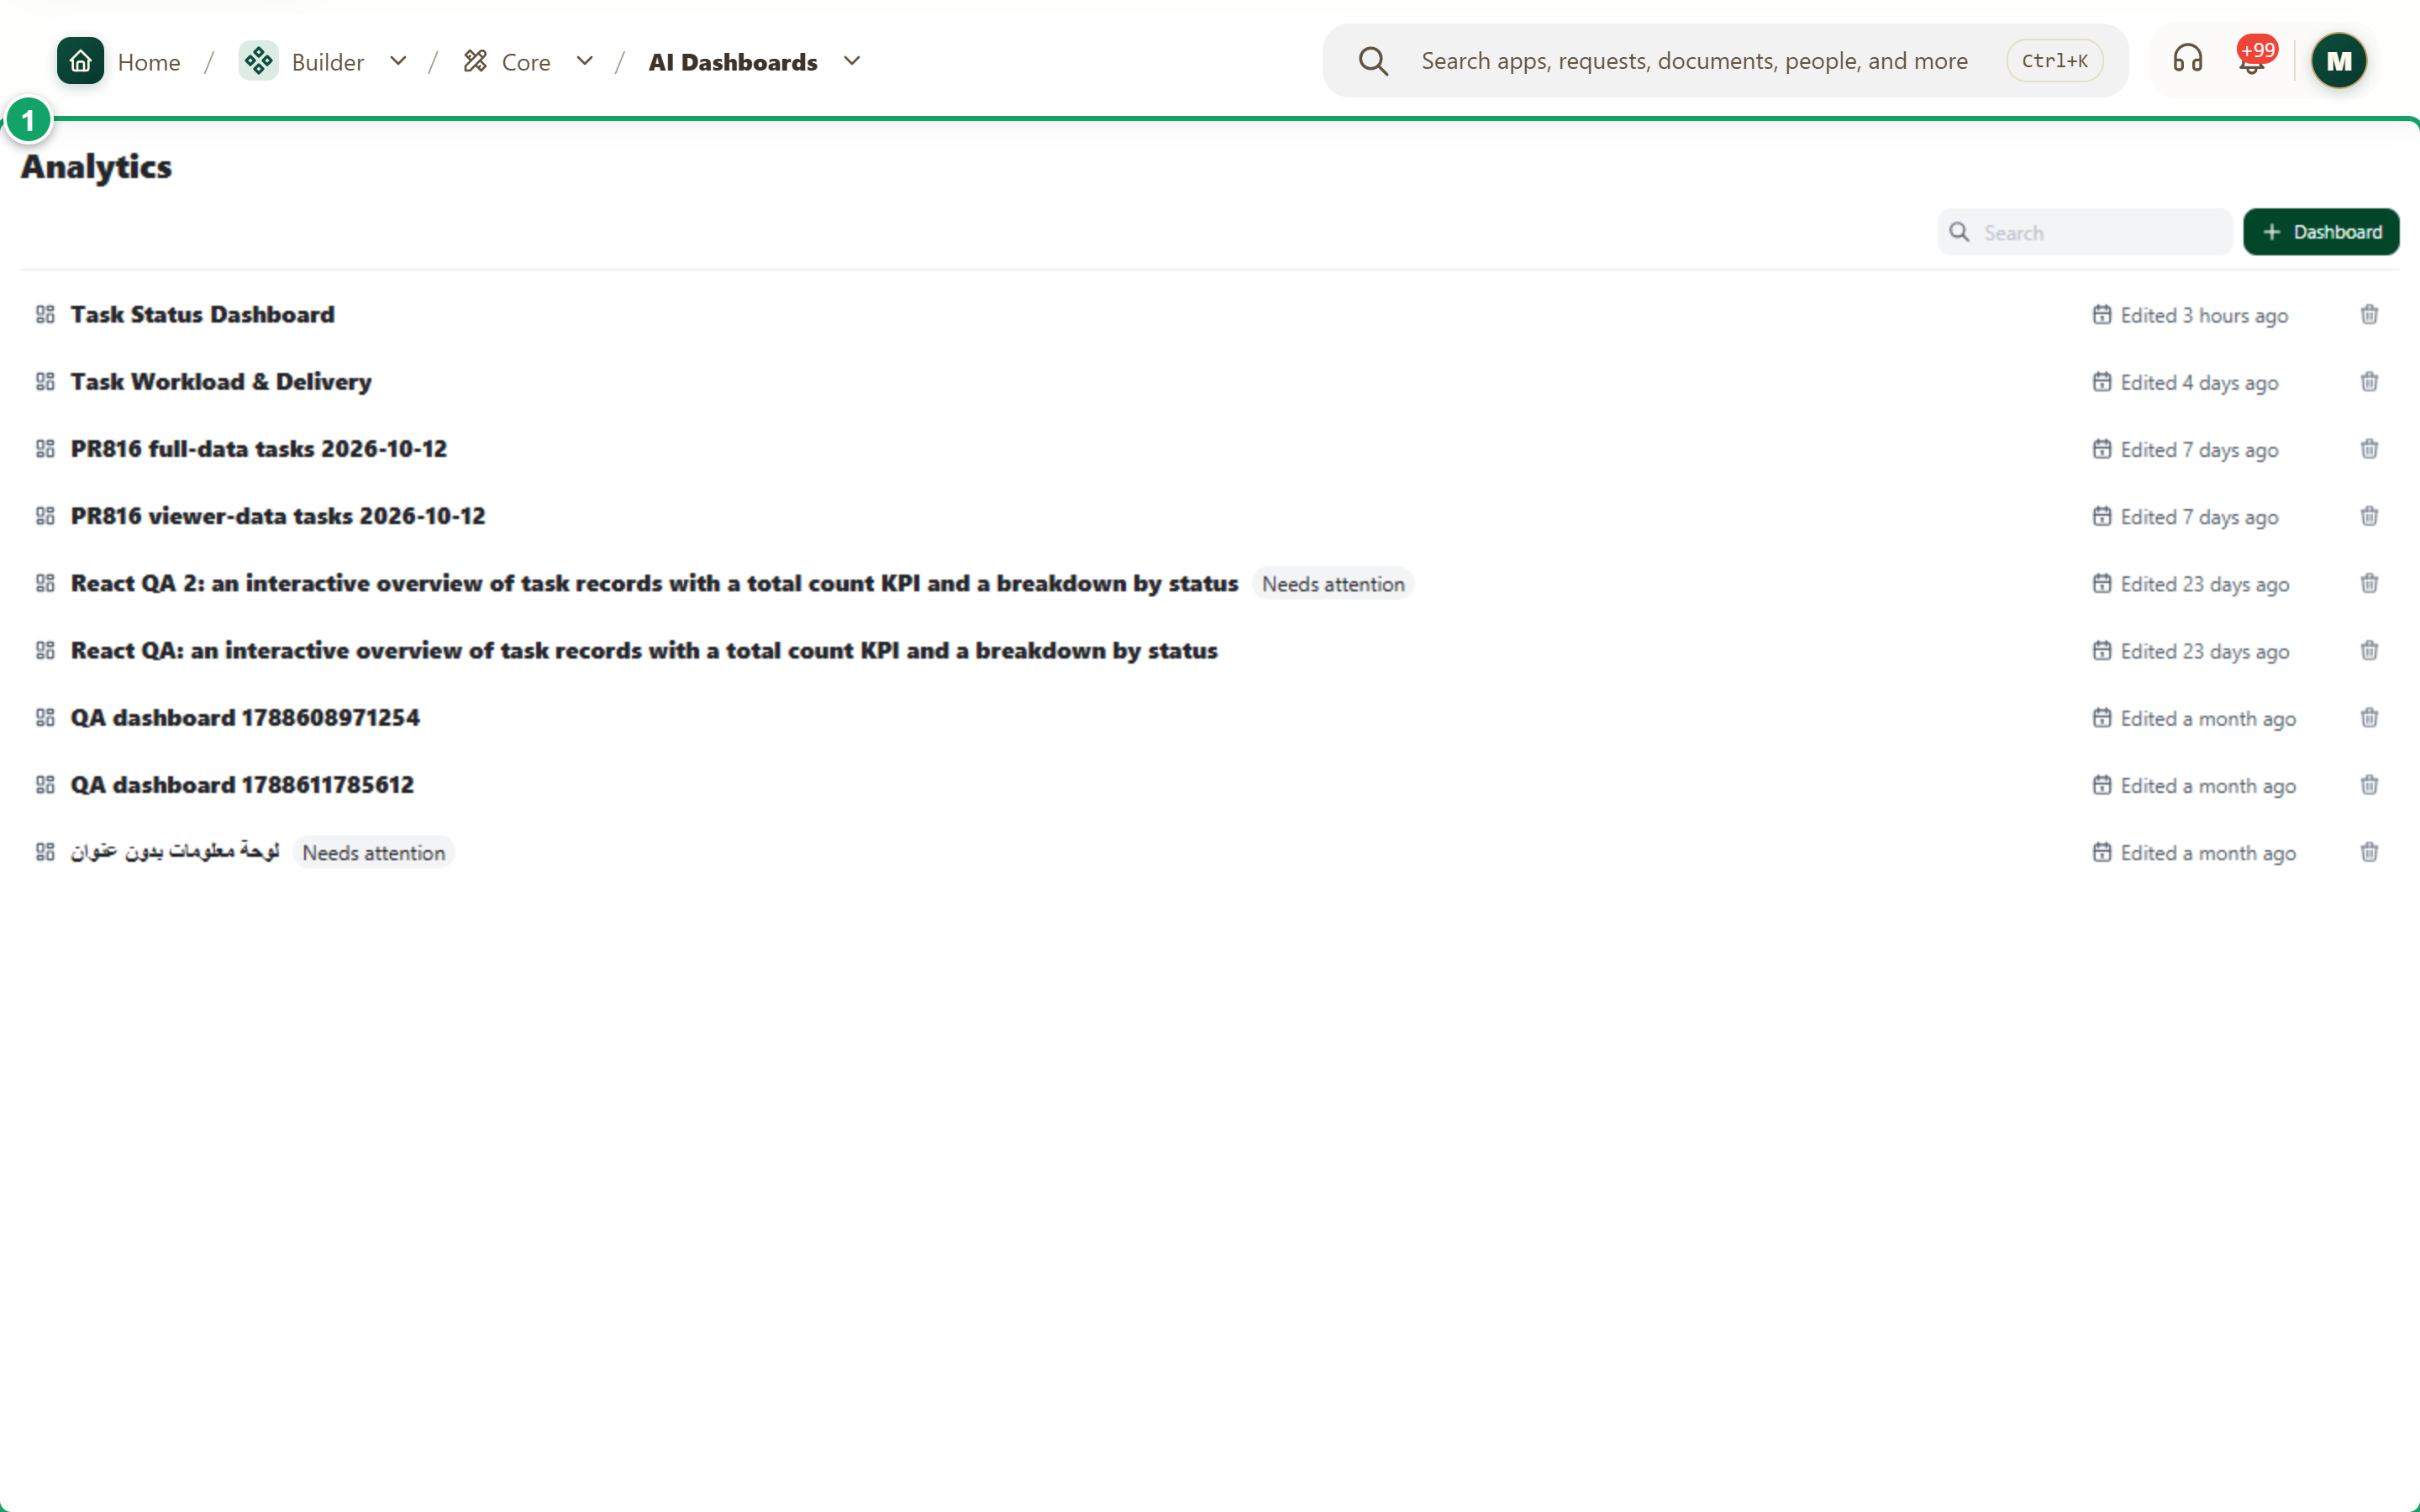
\includegraphics[width=0.95\linewidth,height=0.72\textheight,keepaspectratio]{figures/screens/ch06-ai-dashboards-en.png}
\caption{The “AI Dashboards” workspace}
\label{fig:builder-ai-dashboards-screen}
\shotnote{The analytics workspace opens inside KayanOS and shows the user’s own dashboards. The content here belongs to the test organization. ① The analytics workspace: where dashboards are created and reviewed, served by the embedded analytics system.}
\end{figure}


\begin{table}[H]
\centering
\caption{What should you know?}
\label{tab:builder-ai-dashboards-data}
\begin{tabularx}{\linewidth}{R{3.6cm} Y}
\rcHeaderRow
\thh{Aspect} & \thh{Meaning}\\
Private workspace & Dashboards here are yours alone and are computed only from data you are allowed to read.\\
Unavailable data & A message may say some data is unavailable because your access to certain record types is too broad to include.\\
Sharing & A dashboard is shared by publishing it as a page from “Pages”, not from this workspace.\\
\end{tabularx}
\end{table}

\begin{figure}[H]
\centering
\begin{tikzpicture}[node distance=0.5cm]
\node[stepBox] (a) {Describe what you want to know};
\node[stepBox,below=of a] (b) {Review the dashboard};
\node[stepBox,below=of b] (c) {Publish from Pages if needed};
\draw[flowsTo] (a) -- (b);
\draw[flowsTo] (b) -- (c);
\end{tikzpicture}
\rclegend
\caption{From a question to a shared dashboard}
\label{fig:builder-ai-dashboards-flow}
\shotnote{The diagram puts review before sharing, because an AI-generated dashboard may understand the question differently from what you meant. Compare its numbers with what you know, then share it through “Pages” only when you trust it.}
\end{figure}

\subsection{Steps and check}
\begin{enumerate}
\item Open “AI Dashboards” and wait for the analytics workspace to load.
\item Create a new dashboard and write clearly what you want to know, with the period and the important fields.
\item Review and save the dashboard, then publish it from “Pages” if the team should see it.
\end{enumerate}

\textbf{Check and recovery:} the workspace should open and show your dashboards. If “Could not open analytics” appears or the page sends you back home, your seat does not include analytics or you lack the right to view dashboards; ask the organization administrator.

\clearpage
\section{AI Reports}
\label{sec:builder-feature-ai-reports}

This page opens the same analytics workspace in chat mode: you ask in your own words about the organization's data, and the AI answers with a written report and numbers. It suits quick questions that do not need a permanent dashboard, such as “How many visits were cancelled this month, and why?”.

\textbf{Path and who uses it:} “Builder” → “Core” → “AI Reports”. It is shown under the same conditions as “AI Dashboards”.

\begin{rcnote}[Example: Horizon]
Sarah Al-Khatib asks which branches had visits delayed by more than a week, and gets a short report she uses in the monthly meeting. Sarah asks her question in area ①.
\end{rcnote}

\begin{figure}[H]
\centering
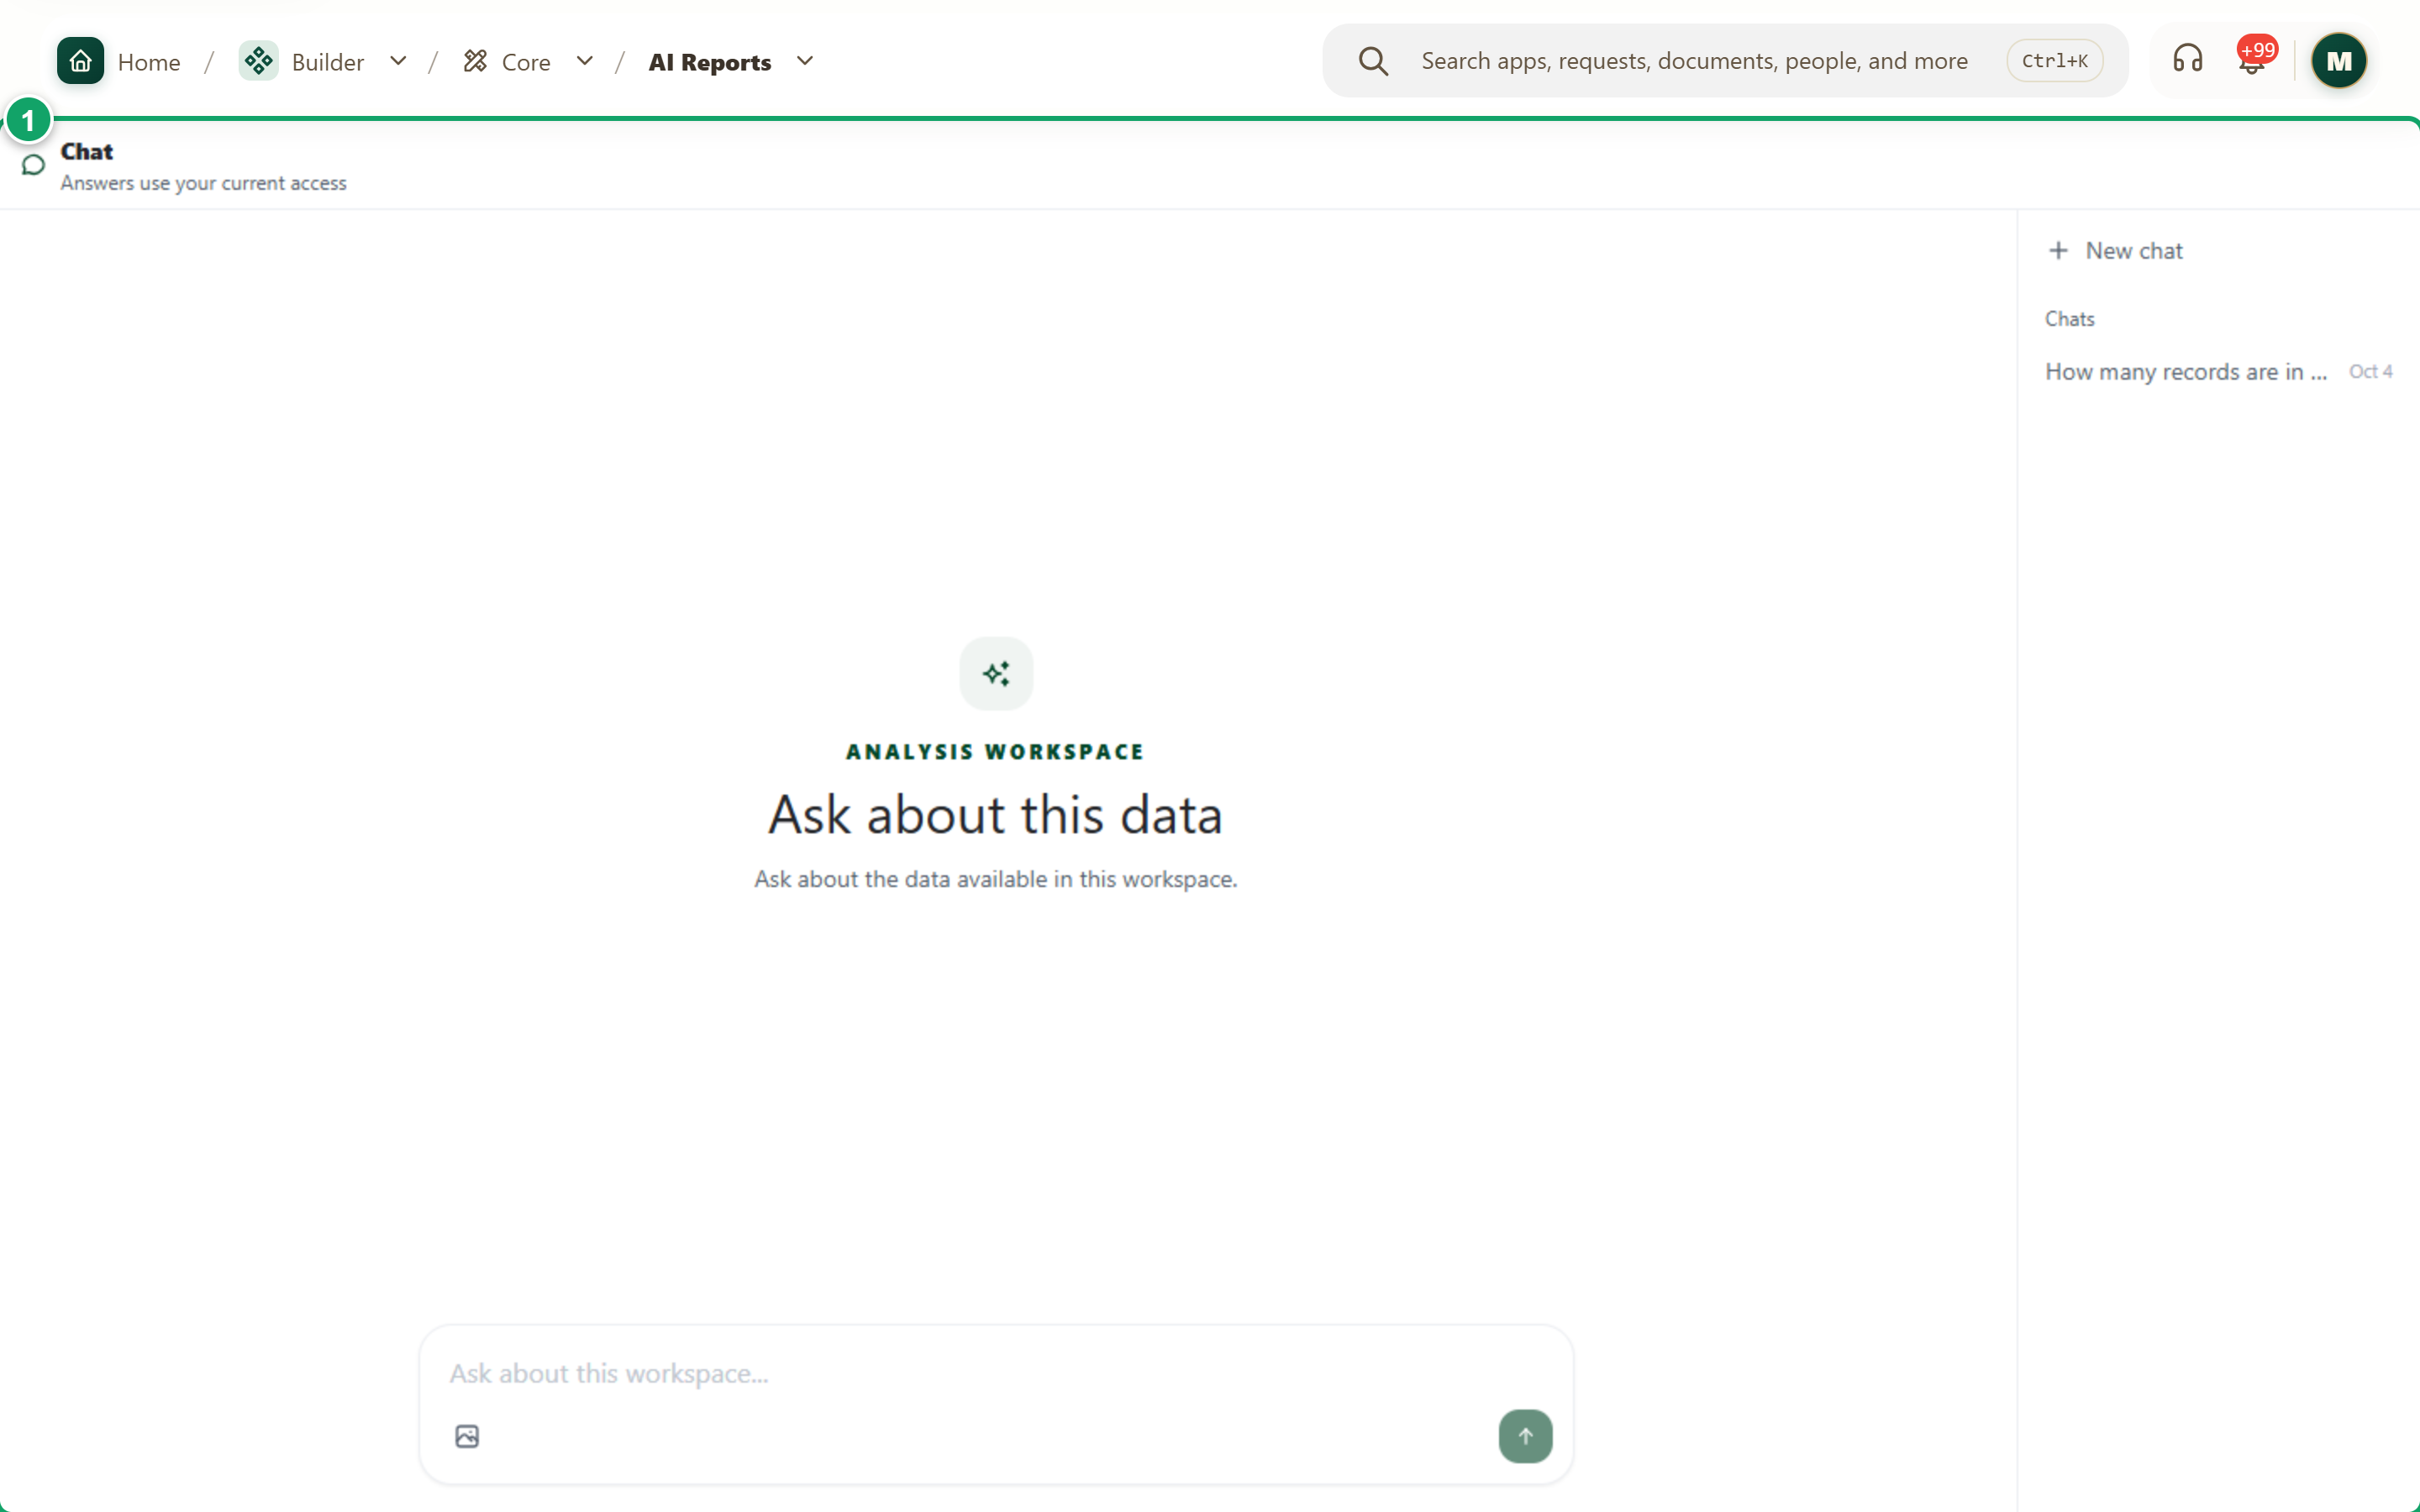
\includegraphics[width=0.95\linewidth,height=0.72\textheight,keepaspectratio]{figures/screens/ch06-ai-reports-en.png}
\caption{The “AI Reports” workspace}
\label{fig:builder-ai-reports-screen}
\shotnote{The same analytics workspace opens in chat mode. ① The chat area: where you write your question and read the report.}
\end{figure}


\begin{table}[H]
\centering
\caption{When to use reports and when to use dashboards}
\label{tab:builder-ai-reports-data}
\begin{tabularx}{\linewidth}{R{3.6cm} Y}
\rcHeaderRow
\thh{Need} & \thh{Best fit}\\
A one-off question & “AI Reports”: ask and read the answer.\\
Recurring follow-up & “AI Dashboards” or “Dashboards”, because a dashboard is refreshed and reviewed regularly.\\
Sharing with the team & Publish the dashboard from “Pages”; chat answers do not appear in navigation.\\
\end{tabularx}
\end{table}

\begin{figure}[H]
\centering
\begin{tikzpicture}[node distance=0.5cm]
\node[stepBox] (a) {A clear question with a period};
\node[stepBox,below=of a] (b) {Read the report};
\node[stepBox,below=of b] (c) {Check one known number};
\draw[flowsTo] (a) -- (b);
\draw[flowsTo] (b) -- (c);
\end{tikzpicture}
\rclegend
\caption{Asking a question and checking the answer}
\label{fig:builder-ai-reports-flow}
\shotnote{The diagram ends with a check, because the answer is built on the data the person asking can read and on how the AI understood the question. If one number you know matches the report, you can trust the rest of the answer more.}
\end{figure}

\subsection{Steps and check}
\begin{enumerate}
\item Open “AI Reports” and wait for the chat to load.
\item Write your question with the time period and the record type you mean.
\item Read the report, and compare one number in it with what you know before relying on it.
\end{enumerate}

\textbf{Check and recovery:} an answer referring to your organization's data should arrive. If the page does not open, review your seat and permissions as for “AI Dashboards”. If the answer looks incomplete, rephrase the question with the record type and period.
